
\def\filedate{2014/12/01}\let\thedate\filedate % packages may change \filedate

\documentclass[11pt,twoside]{article}
\usepackage[obeyspaces]{url}
\usepackage{natbib}
%\usepackage{chem}
\usepackage{color}
\usepackage{rotating} % loads graphicx
\usepackage{longtable}
\usepackage{graphicx}
%\usepackage{verbatim}

\oddsidemargin-5mm
%\evensidemargin-15mm
\evensidemargin-5mm
\topmargin-10mm
\textheight230mm
\textwidth170mm
\raggedbottom
\parindent0mm
\parskip1.0ex plus0.5ex minus0.5ex
\renewcommand{\arraystretch}{1}
\renewcommand{\topfraction}{0.95}
\renewcommand{\dbltopfraction}{0.95}
\renewcommand{\bottomfraction}{0.95}
\renewcommand{\floatpagefraction}{0.95}
\renewcommand{\dblfloatpagefraction}{0.95}
\renewcommand{\textfraction}{0.01}
\setlength{\LTcapwidth}{\textwidth}
\setcounter{topnumber}{3}
\setcounter{secnumdepth}{7}
 \setcounter{tocdepth}{3} 
\newcommand\TODO[1]{\textcolor{red}{#1}}

\newcommand{\egcite}[1]{\citep[e.g.][]{#1}}
\newcommand{\etccite}[1]{\citep[and references therein]{#1}}
\newcommand{\hhline}{\noalign{\vspace{1mm}}\hline\noalign{\vspace{1mm}}}
\newcommand{\hhlines}{\noalign{\vspace{1mm}}\hline\hline\noalign{\vspace{1mm}}}
\newcommand{\kpproot}{{\sc root}}
\newcommand{\todo}[1]{{\uppercase{\bf ((#1))}}}

\def\mypageheader{Kerkweg and J\"ockel: GRID user manual}
\markboth{\mypageheader}{\mypageheader}
\pagestyle{myheadings}

\begin{document}

\thispagestyle{empty}
\vspace*{2cm}
\begin{center}
  {\Huge\bf GRID User Manual}\\[12mm]

\vspace*{2cm}
  {\huge\bf Astrid Kerkweg$^{1,2}$ } 
  {\huge\bf \& Patrick J\"ockel$^3$}\\[9mm]
  \Large
\vspace*{1.5cm}
  $^1$ Institut f\"ur Physik der Atmosph\"are\\
  Johannes Gutenberg Universit\"at Mainz\\
  D-55099 Mainz, Germany\\
  $^2$ now at:  Meteorological  Institute\\
    University Bonn,\\
  Auf dem H\"ugel 20\\ D-53121 Bonn
  \url{kerkweg@uni-bonn.de} \\[0.35cm]

  $^3$ Deutsches Zentrum f\"ur Luft-und Raumfahrt (DLR),\\
   Institut f\"ur Physik der Atmosph\"are, \\
    Oberpfaffenhofen, D-82234 We\ss ling, Germany \\
  \url{patrick.joeckel@dlr.de}


\end{center}

\vfill
{\large This manual is available as electronic supplement of our article
  ``The on-line coupled atmospheric chemistry model system MECO(n)
  – Part 5: Expanding the Multi-Model-Driver (MMD v2.0) for 2-way data
  exchange including data interpolation via GRID (v1.0)'' 
  in Geosci.\ Model Dev.\ 
  (2018), available at: \url{http://www.geosci-model-dev.net}}

\begin{center}
%  Date: \thedate
  Date: \today
\end{center}

\newpage %\twocolumn
\cleardoublepage

\sloppy

\tableofcontents
\clearpage




%+++++++++++++++++++++++++++++++++++++++++++++++++++++++++++++++++++++++++++
%+++++++++++++++++++++++++++++++++++++++++++++++++++++++++++++++++++++++++++
%+++++++++++++++++++++++++++++++++++++++++++++++++++++++++++++++++++++++++++
 \section{Introduction}
This is the User Manual of the generic MESSy submodel GRID. GRID is
 used by submodels requiring grid transformations.
Therefore it is internally used within MESSy and a model user need not
to bother about the technical details of GRID.
However, code developers, implementing grid transformation or other
grid relevant routines into a MESSy code, may find useful information
by reading this manuscript 
as it provides a detailed description of the data
types, the modules and subroutines of GRID and its subsubmodels.
Section 2 gives an overview of how the different subroutines and
modules play together.
The details about all files in the submodel core layer
(SMCL) and the basemodel interface layer (BMIL)  are provided in
 Sects.~\ref{SMCL} and \ref{BMIL}, respectively.

\section{Overview\label{overview}}
Figure \ref{FigGRIDFLOW} depicts the dependencies of the GRID submodel.
The basic GRID modules\footnote{Following the MESSy naming convention,
the Fortran files are named as the modules they contain.}
(\verb|MESSY_MAIN_GRID| and \verb|MESSY_MAIN_GRID_NETCDF|)
 are used by nearly every GRID module (purple arrows). Only the 
subsubmodels GRID\_TRAFO\_SCRP\_BASE is completely autonomeous.
\begin{figure}
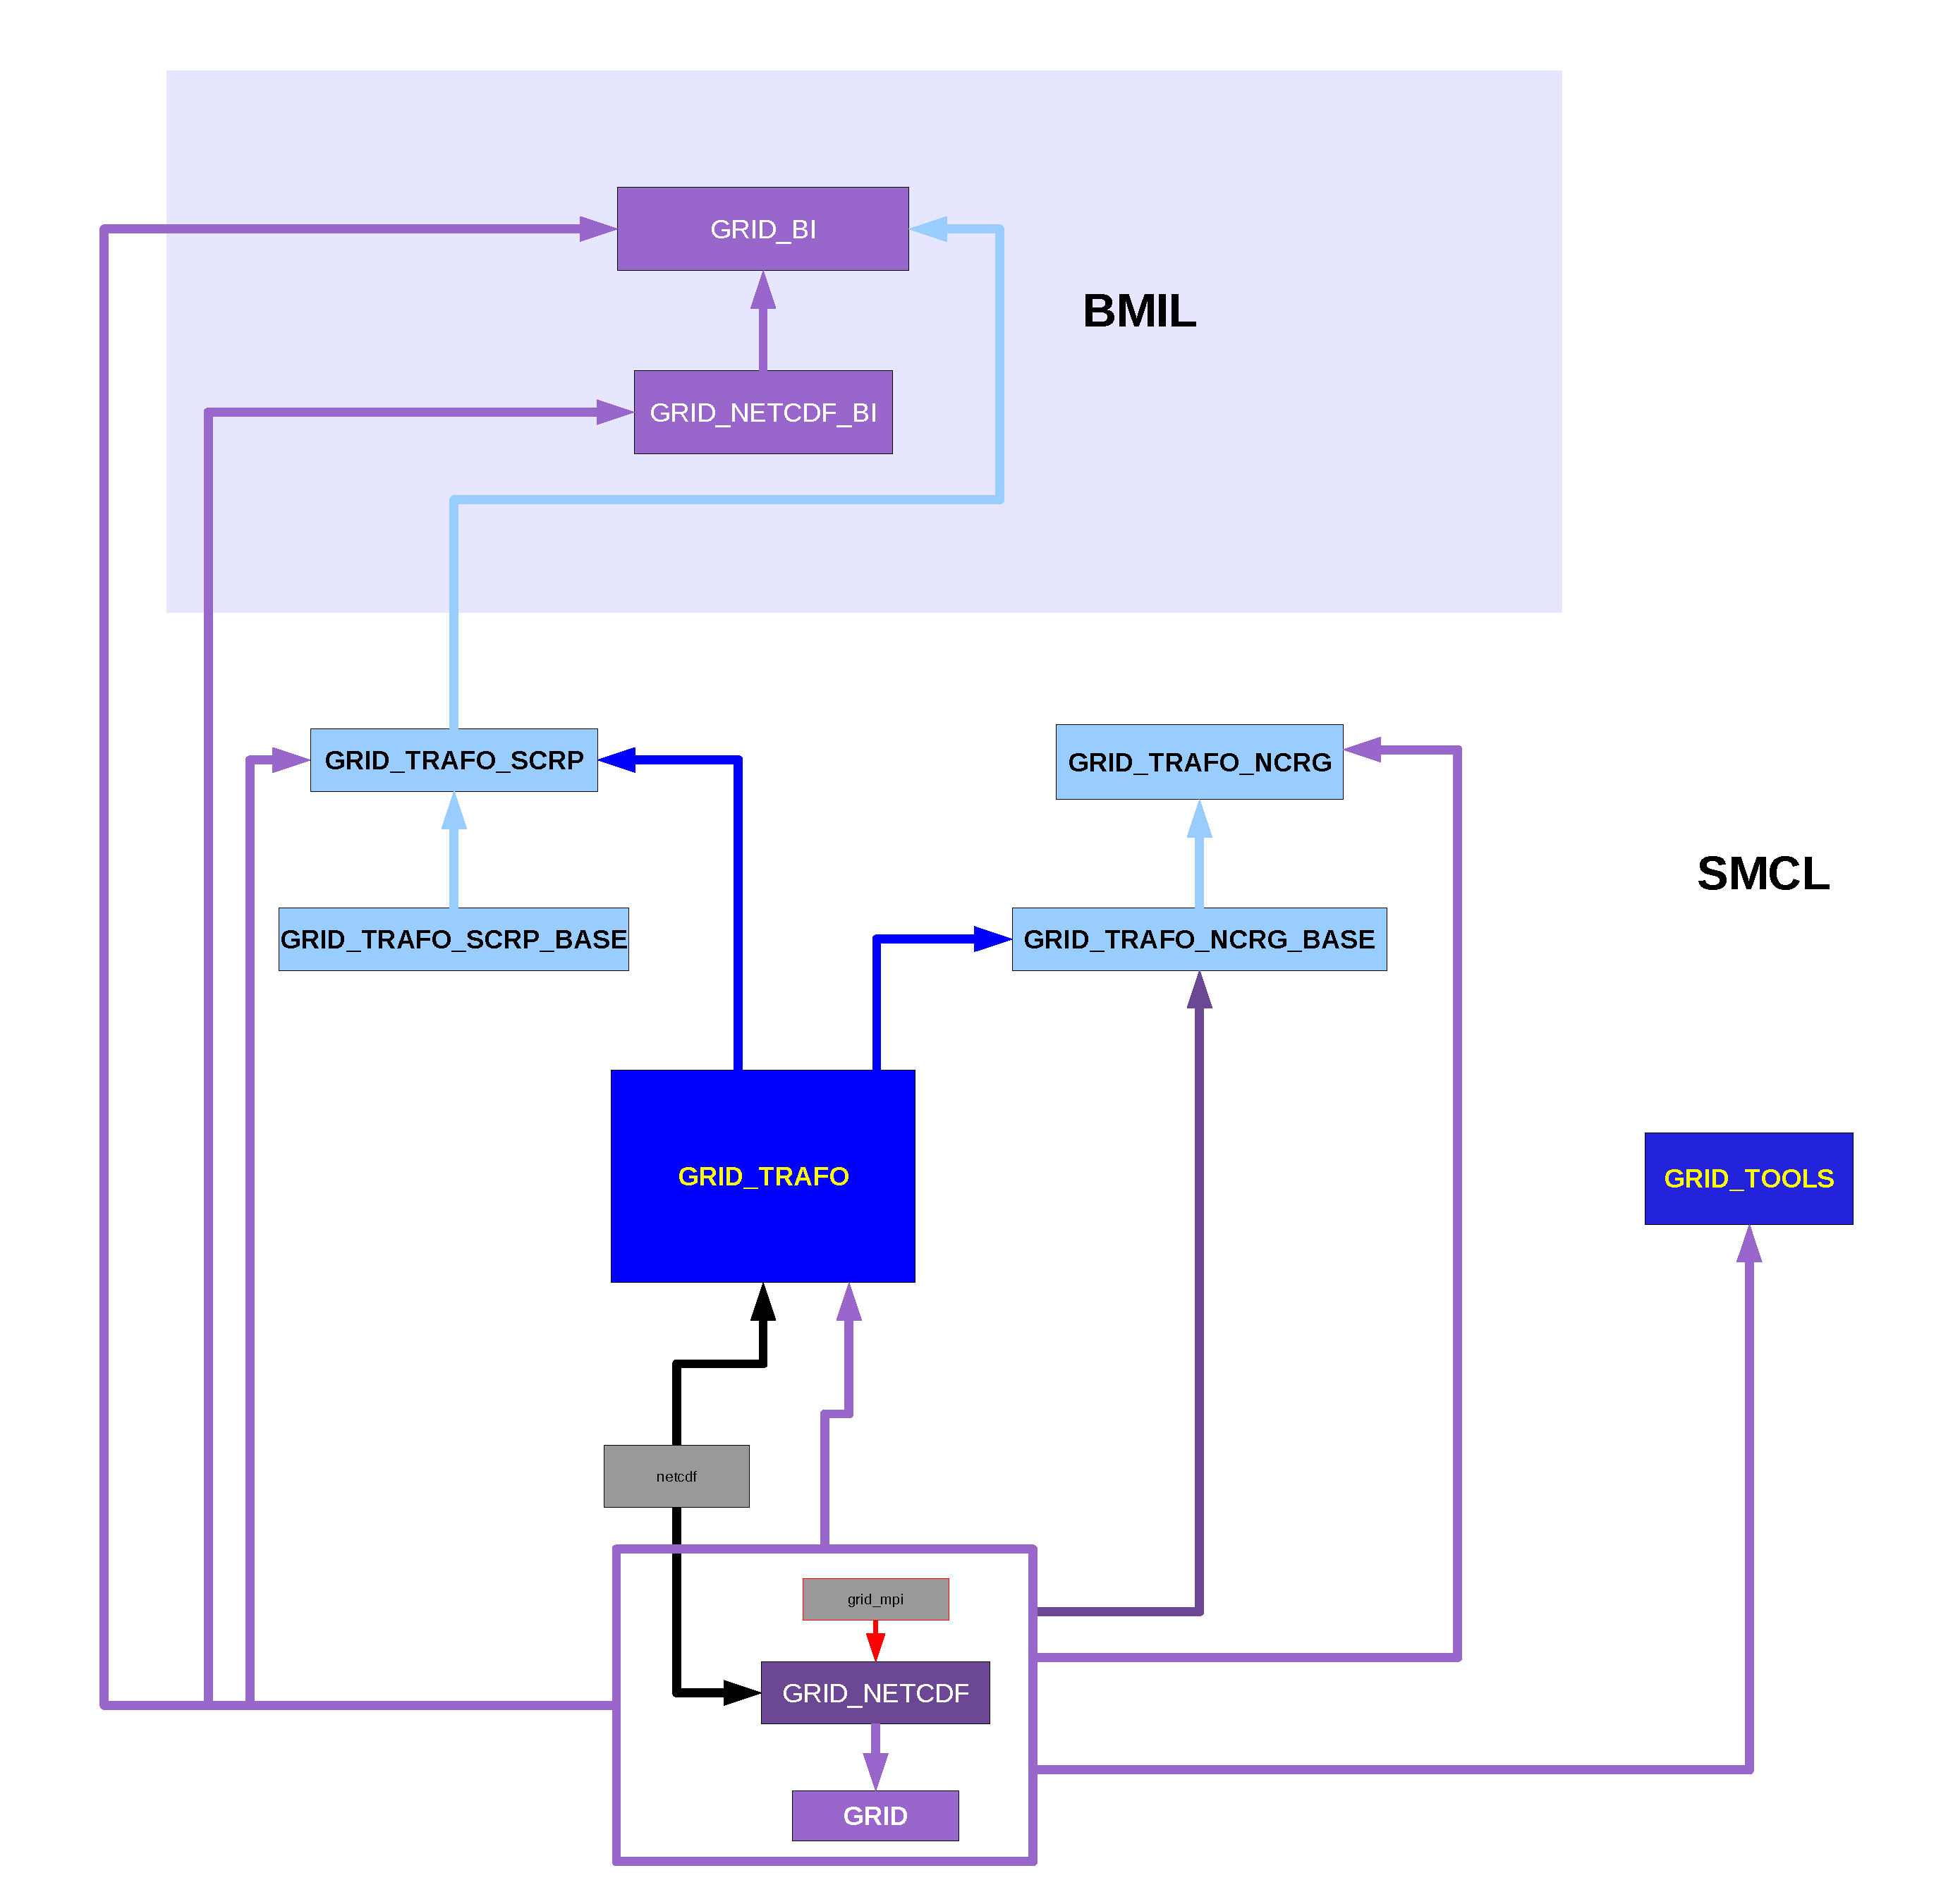
\includegraphics[width=0.95\textwidth]{grid_modules.pdf}
\caption{Diagram of dependencies of the MESSy GRID modules. The
arrows point in the direction of USEage.\label{FigGRIDFLOW}}
\end{figure}

\begin{longtable}{|p{5cm}p{8.5cm}c|}
\caption{List of routines and type declarations in GRID. 
Routines are coloured blue and structures
red.\label{Tab:GRIDroutines}}\\
\hline
\# Routine name & Short description & Sect. \\
\hline
\endfirsthead
\caption{List of routines in GRID (... continued)}\\
\hline
\# Routine name & Short description & Sect. \\
\hline
\endhead
\hline
\endfoot
 & & \\ 
\multicolumn{2}{|c}{\bf \large MESSY\_MAIN\_GRID\_NETCDF}
& \ref{MMGN}\\ \hline 
\color{red} \tt t\_narray & definition of data type array (\verb|t_narray|)& \ref{Tnarray}\\
\color{red} \tt t\_ncdim & definition of data type dimension (\verb|t_ncdim|)& \ref{Tncdim}\\
\color{red} \tt t\_ncatt & definition of data type attribute (\verb|t_ncatt|)& \ref{Tncatt}\\
\color{red} \tt t\_ncvar & definition of data type variable
(\verb|t_ncvar|) & \ref{Tncvar}\\
\color{blue} \tt INIT\_NCDIM & initialisation of a variable of type {\tt t\_ncdim}   & \ref{INITNC}\\
\color{blue} \tt INIT\_NCATT & initialisation of a variable of type {\tt t\_ncatt} & \ref{INITNC}\\
\color{blue} \tt INIT\_NCVAR & initialisation of a variable of type {\tt t\_ncvar}& \ref{INITNC}\\
\color{blue} \tt INIT\_NARRAY & initialisation / allocation of a variable of type {\tt t\_narray}& \ref{INITNARRAY}\\
\color{blue} \tt COPY\_NCDIM & copying of a variable of type {\tt t\_ncdim} & \ref{COPYNC}\\
\color{blue} \tt COPY\_NCATT & copying of a variable of type {\tt t\_ncatt} & \ref{COPYNC}\\
\color{blue} \tt COPY\_NCVAR & copying of a variable of type {\tt t\_ncvar}& \ref{COPYNC}\\
\color{blue} \tt COPY\_NARRAY & copying of a variable of type \verb|t_narray|& \ref{COPYNC}\\
\color{blue} \tt PRINT\_NCDIM & printing of a  variable of type {\tt t\_ncdim} & \ref{PRINTNC}\\
\color{blue} \tt PRINT\_NCATT & printing of a variable of type {\tt t\_ncatt} & \ref{PRINTNC}\\
\color{blue} \tt PRINT\_NCVAR & printing of a variable of type {\tt t\_ncvar}& \ref{PRINTNC}\\
\color{blue} \tt PRINT\_NARRAY & printing of a variable of type \verb|t_narray|& \ref{PRINTNC}\\
\color{blue} \tt QCMP\_NCDIM & comparison of variables of type {\tt t\_ncdim} & \ref{QCMPNC}\\
\color{blue} \tt QCMP\_NCATT & comparison of variables of type {\tt t\_ncatt} & \ref{QCMPNC}\\
\color{blue} \tt QCMP\_NCVAR & comparison of variables of type {\tt t\_ncvar}& \ref{QCMPNC}\\
\color{blue} \tt QCMP\_NARRAY & comparison of variables of type \verb|t_narray|
& \ref{QCMPNC}\\

\color{blue} \tt IMPORT\_NCDIM & import of a variable of type {\tt t\_ncdim} & \ref{IMPNCDIM}\\
\color{blue} \tt IMPORT\_NCATT & import of a variable of type {\tt t\_ncatt}  & \ref{IMPNCATT}\\
\color{blue} \tt IMPORT\_NCVAR & import of a variable of type {\tt t\_ncvar}& \ref{IMPNCVAR}\\
\color{blue} \tt EXPORT\_NCDIM & export of a variable of type {\tt t\_ncdim} & \ref{EXPNC}\\
\color{blue} \tt EXPORT\_NCATT & export of a variable of type  {\tt t\_ncatt} & \ref{EXPNC}\\
\color{blue} \tt EXPORT\_NCVAR & export of a variable of type {\tt t\_ncvar}& \ref{EXPNC}\\
\color{blue} \tt ADD\_NCATT & definition of an attribute variable & \ref{ADDNCATT}\\
\color{blue} \tt QDEF\_NCVAR & check of definition status of variable of type {\tt t\_ncvar}& \ref{QDVAR}\\
\color{blue} \tt SCAN\_NCVAR & import of all variables contained in a
netCDF file& \ref{SCVAR}\\
\color{blue} \tt RENAME\_NCVAR & renaming of a variable of type \verb|t_ncvar|& \ref{RNVAR}\\
\color{blue} \tt IDX2FRAC\_NCVAR& preparation for 'IXF' and 'IDX' remapping& \ref{IDX2FRAC}\\
\color{blue} \tt MAXFRAC2IDX\_NCVAR& postprocessing of data required
for 'IDX' remapping & \ref{MFRAC2IDX}\\
\color{blue} \tt EXTRACT\_NCATT & conversion of GRID to CHANNEL attributes & \ref{EXTATT}\\
\color{blue} \tt NFERR & output of netCDF error messages & \ref{NFERR}\\
\color{blue} \tt STRING & conversion of a 1D character pointer to string & \ref{STR}\\
\color{blue} \tt SORT\_NARRAY & Sorting of a 1D variable of
type \verb|t_narray|& \ref{SORT}\\
\color{blue} \tt REORDER\_NARRAY & Reordering of a variable of
type \verb|t_narray|& \ref{REORDER}\\
\color{blue} \tt DP\_NARRAY & conversion of a variable of type \verb|t_narray|
 to double precision float (\verb|VTYPE_DOUBLE|) & \ref{DPARRAY}\\
\color{blue} \tt SP\_NARRAY & conversion of a variable of type \verb|t_narray|
 to single precision float (\verb|VTYPE_REAL|) & \ref{SPARRAY}\\
\color{blue} \tt SCALE\_NARRAY & Scaling of a variable of type \verb|t_narray| & \ref{SCALEARRAY}\\
\color{blue} \tt CAT\_NARRAY & merging of two variables of type \verb|t_narray| & \ref{CATARRAY}\\
\color{blue} \tt POSITION & calculation of position number in 1D array & \ref{POS}\\
\color{blue} \tt ELEMENT & calculation of the element vector of an
element of given position & \ref{ELEMENT}\\
\color{blue} \tt QSORT\_I & sorting of a 1D integer data array & \ref{QSORT}\\
\color{blue} \tt QSORT\_B & sorting of a 1D byte data array & \ref{QSORT}\\
\color{blue} \tt QSORT\_R & sorting of a 1D single precision data array & \ref{QSORT}\\
\color{blue} \tt QSORT\_D & sorting of a 1D double precision data array & \ref{QSORT}\\
\color{blue} \tt ERRMSG & error handling subroutine & \ref{ERRMSG}\\
\color{blue} \tt RGMSG & interface of message system & \ref{RGMSG}\\
\color{blue} \tt MAIN\_GRID\_SET\_MESSAGEMODE & definition of
verbosity of \verb|RGMSG| & \ref{SETMODE}\\
\color{blue} \tt {NARRAYMAXVAL} & determination of the maximum  value
of the \verb|dat|
component for a given variable of type \verb|t_narray| & \ref{NARRVAL}\\
\color{blue} \tt {NARRAYMINVAL} &  determination of the minimum  value
of the \verb|dat|
component for a given variable of type \verb|t_narray| & \ref{NARRVAL}\\
 & & \\ 
\multicolumn{2}{|c}{\bf \large MESSY\_MAIN\_GRID}& \ref{MMG}\\ \hline 
\color{red} \tt t\_geohybgrid & definition of data type for geohybrid
 grids& \ref{Tghgrid}\\
\color{blue} \tt {INIT\_GEOHYBGRID} & initialisation of a variable of
type \verb|t_geohybgrid| & \ref{INITGHG}\\
\color{blue} \tt {COPY\_GEOHYBGRID} & copying of a variable of
type \verb|t_geohybgrid| & \ref{COPYGHG}\\
\color{blue} \tt {PRINT\_GEOHYBGRID} & printing of a variable of
type \verb|t_geohybgrid| & \ref{PRNTGHG}\\
\color{blue} \tt {IMPORT\_GEOHYBGRID} & import of a  variable of
type \verb|t_geohybgrid| & \ref{IMPGRID}\\
\color{blue} \tt {EXPORT\_GEOHYBGRID} & export of a variable of
type \verb|t_geohybgrid| & \ref{EXPGRID}\\
\color{blue} \tt {NEW\_GEOHYBGRID} & definition of a new grid of
type \verb|t_geohybgrid| & \ref{NEWGRID}\\
\color{blue} \tt {COMPARE\_TO\_GRID} & comparison of a grid of
type \verb|t_geohybgrid| to given grid components& \ref{CMP2GRID}\\
\color{blue} \tt {LOCATE\_GEOHYBGRID} & location of grid of
type \verb|t_geohybgrid| in concatenated list of grids & \ref{LOCGRID}\\
\color{blue} \tt {CLEAN\_GEOHYBGRID\_LIST} & deletion of the concatenated list
of geohybrid grids & \ref{CLEANGRIDL}\\
\color{blue} \tt {GRID\_ERROR} & error function & \ref{GRIDERR}\\
 & & \\ 
\multicolumn{2}{|c}{\bf \large MESSY\_MAIN\_GRID\_TRAFO}& \ref{MMGT}\\ \hline 
\color{blue} \tt {SWITCH\_GEOHYBGRID} & deletion of spacial dimensions
from a grid of type \verb|t_geohybgrid| & \ref{SWITCHGRID}\\
\color{blue} \tt {CHECK\_GEOHYBGRID} & consistency check for
components of a grid of type \verb|t_geohybgrid| & \ref{CHECKGRID}\\
\color{blue} \tt {SORT\_GEOHYBGRID} & sorting of individual grid
components from smallest to largest & \ref{SORTGRID}\\
\color{blue} \tt {H2PSIG} & calculation of sigma or pressure levels
from hybgrid pressure coordinates & \ref{H2PSIG}\\
\color{blue} \tt {COMPLETE\_GEOHYBGRID} & consistent definition of
mid-points and interfaces in a grid  of
type \verb|t_geohybgrid| & \ref{COMPLETEGRID}\\
\color{blue} \tt {CHECK\_VAR\_ON\_GEOHYBGRID} & check if a variable of
type \verb|t_ncvar| is defined on a grid of type \verb|t_geohybgrid|
& \ref{CHKVARONGRID}\\ 
\color{blue} \tt {SORT\_GEOHYBGRID\_NCVAR} & sorting of  a variable of
type \verb|t_ncvar| according to a sorted grid of type \verb|t_geohybgrid|
& \ref{SORTGRIDVAR}\\ 
\color{blue} \tt {PACK\_GEOHYBGRID\_NCVAR} & packing of a variable of
type \verb|t_ncvar| according to axes and dimension information 
& \ref{PACKGRIDVAR}\\ 
\color{blue} \tt {BALANCE\_GEOHYBGRID} & copying of components of one
grid of type \verb|t_geohybgrid| to another & \ref{BALGRID}\\ 
\color{blue} \tt {BALANCE\_GEOHYBGRID\_NCVAR} & dimensioning of a
variable of type \verb|t_ncvar| according to a
grid of type \verb|t_geohybgrid| & \ref{BALGRIDVAR}\\ 
\color{blue} \tt {BALANCE\_GEOHYBGRID\_TIME} & adjustment of the time
axis of two grids  of type \verb|t_geohybgrid| & \ref{BALGRIDTIME}\\ 
\color{blue} \tt {REDUCE\_INPUT\_GRID} & reduction of input grid  of type \verb|t_geohybgrid| & \ref{REDINPGRID}\\ 
\color{blue} \tt {PHIROT2PHI} & calculation of (geographical) latitude & \ref{PR2P}\\ 
\color{blue} \tt {PHI2PHIROT} & calculation of rotated latitude & \ref{P2PR}\\ 
\color{blue} \tt {RLAROT2RLA} & calculation of (geographical) longitude & \ref{LR2L}\\ 
\color{blue} \tt {RLAROT2RLA} & calculation of rotated longitude& \ref{L2LR}\\ 
\color{blue} \tt {UVROT2UV} & conversion of rotated wind vector to
geographical wind vector  & \ref{windconv}\\ 
\color{blue} \tt {UV2UVROT} & conversion of geographical wind vector to
rotated wind vector  & \ref{windconv}\\ 
\color{blue} \tt {UVROT2UV\_VEC\_JLOOP} & conversion of rotated wind vector to
geographical wind vector operating on j-vector  & \ref{windconv}\\ 
 & & \\ 
 & & \\ 
 & & \\ 
 & & \\ 
\multicolumn{2}{|c}{\bf \large MESSY\_MAIN\_GRID\_TOOLS}& \ref{MMGTO}\\ \hline 
\color{blue} \tt {RGTOOL\_CONVERT} & conversion of a variable of
 type \verb|t_ncvar| to a 4D array & \ref{RGTCONV}\\ 
\color{blue} \tt {RGTOOL\_CONVERT\_DAT2VAR} & conversion of a 4D array
to a variable of type \verb|t_ncvar| & \ref{RGTCONVD2V}\\ 
\color{blue} \tt {RGTOOL\_G2C} & conversion of grid components to
multi-dimensional arrays & \ref{RGTG2C}\\ 
\color{blue} \tt {ALINE\_ARRAY} & conversion of a 2D array to a 1D vector & \ref{ALARRAY}\\ 
\color{blue} \tt {DEALINE\_ARRAY} & conversion of a 1D vector to a 2D array & \ref{DEALARRAY}\\ 
\color{blue} \tt {SET\_SURFACE\_PRESSURE} & (re-)setting of surface
pressure component in a grid of type \verb|t_geohybgrid|  & \ref{SETSPRESS}\\ 
 & & \\ 
\multicolumn{2}{|c}{\bf \large MESSY\_MAIN\_GRID\_TRAFO\_NRGD\_BASE}& \ref{MMGTNB}\\ \hline 
 & & \\ 
\multicolumn{2}{|c}{\bf \large MESSY\_MAIN\_GRID\_TRAFO\_NRGD}& \ref{MMGTN}\\ \hline 
\color{blue} \tt {REGRID\_CONTROL} & driver of remapping by NREGRID & \ref{RGRDCNTRL}\\ 
\color{blue} \tt {GEOHYBGRID\_AXES} & construction of axes from grid information& \ref{GRIDAXES}\\ 
\color{blue} \tt {PS2PS} & extraction of a variable of
type \verb|t_narray| from a variable of type \verb|t_ncvar| & \ref{PS2PS}\\ 
\color{blue} \tt {BALANCE\_GEOHYBGRID\_PS} & adjustment of the surface
pressure fields of two grids & \ref{BALGRIDPS}\\ 
\color{blue} \tt {REGRID\_GEOHYBGRID\_PS} & mapping of the surface
pressure field of one grid to another grid & \ref{RGDGRIDPS}\\ 
 & & \\ 
\multicolumn{2}{|c}{\bf \large MESSY\_MAIN\_GRID\_TRAFO\_SCRP\_BASE}& \ref{MMGTSB}\\ \hline 
 & & \\ 
\multicolumn{2}{|c}{\bf \large MESSY\_MAIN\_GRID\_TRAFO\_SCRP}& \ref{MMGTS}\\ \hline 
\color{red} \tt t\_scrip\_grid & definition of a structure describing a SCRIP grid & \ref{Tsgrid}\\
\color{red} \tt t\_scrip\_data & definition of a structure combining
two SCRIP grids, a mapping method and the corresponding weights & \ref{Tsdata}\\
\color{red} \tt t\_scrip\_weights & structure containing SCRIP weights & \ref{Tsweights}\\
\color{blue} \tt {INIT\_SCRIPGRID} &  (re-)initialisation of a grid of
type \verb|t_scrip_grid|& \ref{INITSG}\\ 
\color{blue} \tt {COPY\_SCRIPGRID} & copying of one  grid of
type \verb|t_scrip_grid| to another grid of the same type & \ref{COPYSG}\\ 
\color{blue} \tt {DEFINE\_SCRIPGRID} & definition of a grid of
type \verb|t_scrip_grid| & \ref{DEFSG}\\ 
\color{blue} \tt {CLEAN\_SCRIPGRID\_LIST} & deletion of the  concatenated list
of grids of type \verb|t_scrip_grid| & \ref{CLEANSGL}\\ 
\color{blue} \tt {COMPARE\_TO\_SCRIPGRID} & comparison of grid components
to a grid of type  \verb|t_scrip_grid| & \ref{CTG}\\ 
\color{blue} \tt {GEOHYB2SCRIPGRID} & conversion of a grid of
type \verb|t_geohybgrid| to a grid of type \verb|t_scrip_grid| & \ref{GH2SG}\\ 
\color{blue} \tt {INIT\_SCRIPDATA} &  (re-)initialisation of a
structure of type \verb|t_scrip_data|& \ref{INITSD}\\ 
\color{blue} \tt {DEFINE\_SCRIPDATA} & definition of a variable of
type \verb|t_scrip_data|& \ref{DEFSD}\\  
\color{blue} \tt {COMPARE\_SCRIPDATA} & comparison of individual
components to a SCRIP data set of type \verb|t_scrip_data|& \ref{CMPSD}\\  
\color{blue} \tt {LOCATE\_SCRIPDATA} & location of a SCRIP data set of
type \verb|t_scrip_data| in the concatenated SCRIP data list& \ref{LOCSD}\\  
\color{blue} \tt {CLEAN\_SCRIPDATA\_LIST} & deletion of the concatenated list
of data sets of type \verb|t_scrip_data| & \ref{CLEANSDL}\\ 
\color{blue} \tt {CALC\_SCRIPDATA} & definition of a SCRIP data set of type \verb|t_scrip_data|& \ref{CALCSD}\\  
\color{blue} \tt {INIT\_WEIGHTS} & re-initialisation of a variable of
type \verb|t_scrip_weights|& \ref{INITWEIGHTS}\\  
\color{blue} \tt {CALC\_SCRIP\_WEIGHTS} & calculation of the weights
component of a SCRIP data set & \ref{CALCWEIGHTS}\\  
\color{blue} \tt {APPLY\_SCRIP\_WEIGHTS} & SCRIP interpolation & \ref{APPLYSWEIGHTS}\\  
\color{blue} \tt {SCRIP\_CONTROL} & driver of remapping by SCRIP & \ref{SCRPCNTRL}\\  
\color{blue} \tt {INTERPOL\_GEOHYBGRID\_PS} &  interpolation of a surface
pressure fields defined on one grid to another grid of type \verb|t_scrip_grid|  & \ref{IGHPS}\\  
\color{blue} \tt {BALANCE\_CURVILINEAR\_PS} &  adjustment of the
surface pressure definition of two grids & \ref{BALCLPS}\\  
\color{blue} \tt {\small CONSTRUCT\_INPUT\_SURF\_PRESSURE} & definition of a
surface pressure component for a grid & \ref{CONSTISPS}\\  
 & & \\ 
\multicolumn{2}{|c}{\bf \large
 MESSY\_MAIN\_GRID\_MPI}& \ref{MMGMPI}\\ \hline
 & & \\ \hline 
 & & \\ 
\multicolumn{2}{|c}{\bf \large MESSY\_MAIN\_GRID\_BI}& \ref{MMGBI}\\ \hline 
\color{blue} \tt {P\_BCAST\_GRID} &  broadcasting of a grid of
type \verb|t_geohybgrid| & \ref{PBCGRID}\\  
\color{blue} \tt {MAIN\_GRID\_INIT\_MEMORY} & allocation of memory & \ref{MGIM}\\  
\color{blue} \tt {MAIN\_GRID\_FREE\_MEMORY} & deallocation of memory & \ref{MGFM}\\  
 & & \\ 
\multicolumn{2}{|c}{\bf \large MESSY\_MAIN\_GRID\_NETCDF\_BI}& \ref{MMGCDFBI}\\ \hline 
\color{blue} \tt {P\_BCAST\_NCVAR} & broadcasting of a variable of type \verb|t_ncvar| & \ref{PBCVAR}\\  
\color{blue} \tt {P\_BCAST\_NCATT} & broadcasting of a variable of type \verb|t_ncatt| & \ref{PBCARR}\\  
\color{blue} \tt {P\_BCAST\_NCDIM} & broadcasting of a variable of type \verb|t_ncdim| & \ref{PBCDIM}\\  
\color{blue} \tt {P\_BCAST\_NARRAY} & broadcasting of a variable of type \verb|t_narray| & \ref{PBCARR}\\  
\end{longtable}
\vspace*{0.5cm}

\section{The SMCL GRID files\label{SMCL}}
In the hierarchy of the GRID SMCL
modules \verb|MESSY_MAIN_GRID_NETCDF| is the most basic one.  
It provides the netCDF related type declarations and corresponding 
 routines. 
The structures are used as components of more complex structures. 
They build the basis for all other process routines. 
Additionally, \verb|MESSY_MAIN_GRID_NETCDF| contains the error output
routines. 

The module \verb|MESSY_MAIN_GRID| contains the definition and the 
handling routines of the geohybrid grid. For this, the
structures declared in  \verb|MESSY_MAIN_GRID_NETCDF| are used.
The geohybrid grid definition and respective handling routines are
the basis for the grid transformation.

The actual grid transformation routines are split into seven modules:
\begin{itemize}
\item Each individual mapping algorithm 
 (at the time being SCRIP and NREGRID) consists of two module files:
\begin{itemize}
\item a ``\verb|base|'' file, containing the code of the actual 
regridding algorithm and
\item the interface file that calls those core routines and contains
the subroutines required for the pre- and postprocessing of the input
 and output to/from the core, according to the requirements of the respective 
regridding algorithm.
\end{itemize}
\item In addition to the mapping algorithm dependent modules, one module 
(\verb|MESSY_MAIN_GRID_TRAFO|) provides tools for data operations
which are independent of the mapping method.
\item The module \verb|MESSY_MAIN_GRID_TOOLS| contains tools for
conversions between the internally used 1D storage format and the user
defined 2D and 4D arrays, which are attributed to geo-spacial grids of the
respective model.
Furthermore, a subroutine is provided for updating the surface pressure field
contained in the grid definition during the simulation.

\item Last but not least, the module \verb|MESSY_MAIN_GRID_MPI|
comprises routines for the proper abortion of the simulations, e.g., in
case of error, in parallel mode. 
\end{itemize}

%*********************************************************************
\subsection{MESSY\_MAIN\_GRID\_NETCDF \label{MMGN}}

\subsubsection{GRID data types}
The layout of the basic GRID data types is based on the netCDF file
format definition.
Thus structures for data arrays (\verb|t_narray|), dimensions 
(\verb|t_ncdim|), attributes (\verb|t_ncatt|) and variables (\verb|t_ncvar|)
are defined here.

\paragraph{TYPE t\_narray\label{Tnarray}\\}
\begin{table}[t]
\begin{center}
%\begin{tabular}{|p{3cm}p{2.cm}p{10cm}|}\hline
\begin{tabular}{|lcp{10cm}|}\hline
Parameter& pointer  &type / meaning\\
  name &  name in & \\
       & \verb|t_narray| &\\\hline
\verb|VTYPE_UNDEF|  &&  undefined, i.e. none of the pointers in the variable of type \verb|t_narray| is associated\\
\verb|VTYPE_INT|    & \verb|vi|& the integer pointer is associated\\
\verb|VTYPE_REAL|   & \verb|vr| &the single precision pointer is associated\\
\verb|VTYPE_DOUBLE| & \verb|vd| &the double precision pointer is associated\\
\verb|VTYPE_BYTE|   & \verb|vb| &the byte value (integer I4) pointer is associated\\
\verb|VTYPE_CHAR|   & \verb|vc| &the character pointer is associated \\\hline
\end{tabular}
\caption{Table of variable types available in variables of the type
  {\rm t\_narray }\label{typetab}}
\end{center}
\end{table}
The type \verb|t_narray| defines a universal data array. 
Universal means here, that each data type can be used.
For this, the type definition contains a vector pointer for each basic
data type: single
 precision float (\verb|vr|), double precision float (\verb|vd|),
 integer(I8) (\verb|vi|), integer(I4) or byte  (\verb|vb|),
and characters (\verb|vc|).
\begin{verbatim}
!-----------------------------------------------------------------------------------
  TYPE t_narray
     ! n-dimenional array as 1D (LINEAR) array (REAL)
     INTEGER                              :: type = VTYPE_UNDEF
     INTEGER                              :: n = 0         ! number of dimensions
     INTEGER     , DIMENSION(:), POINTER  :: dim => NULL() ! dim. vector
     REAL (SP)   , DIMENSION(:), POINTER  :: vr  => NULL() ! real values
     REAL (DP)   , DIMENSION(:), POINTER  :: vd  => NULL() ! double values
     INTEGER (I8), DIMENSION(:), POINTER  :: vi  => NULL() ! integer values
     INTEGER (I4), DIMENSION(:), POINTER  :: vb  => NULL() ! byte values
     CHARACTER,    DIMENSION(:), POINTER  :: vc  => NULL() ! char. values
  END TYPE t_narray
!-----------------------------------------------------------------------------------
\end{verbatim}
Only one of the pointers will become associated, when a variable of type 
\verb|t_narray| is defined. All other pointers are nullified. 
The integer component \verb|type| indicates which of the data pointers is 
associated (see Table \ref{typetab} for a
list of the possible values of \verb|type|),
and the variable \verb|n| contains the length of the data array.
The integer parameter \verb|VTPYE_UNDEF| is zero and indicates, if
currently no data is associated.
The component \verb|dim| is a vector which is allocated to the number
of ranks of the corresponding user variable. Each entry
of \verb|dim| contains the length of that respective dimension.


%\paragraph{\textcolor{magenta}{t\_ncdim}\label{Tncdimy}\\}
\paragraph{{t\_ncdim}\label{Tncdim}\\}
The structure \verb|t_ncdim| contains information to describe
 a dimension as in the netCDF standard.

\begin{verbatim}
!-----------------------------------------------------------------------------------
  TYPE t_ncdim
     CHARACTER(LEN=GRD_MAXSTRLEN) :: name = ''    ! name of dimension
     INTEGER                :: id    = NULL_DIMID ! dimension ID
     INTEGER                :: len   = 0          ! length of dimension
     LOGICAL                :: fuid  = .false.    ! flag for "UNLIMITED" dimension
     INTEGER                :: varid = NULL_VARID ! variable ID, if coordinate var
  END TYPE t_ncdim
!-----------------------------------------------------------------------------------
\end{verbatim}
This structure consists of 
\begin{itemize}
\item a (unique) \verb|name|, 
\item an ID (\verb|id|) indicating the dimension distinctively,
\item the length of the dimension (\verb|len|),
\item a logical flag (\verb|fiud|) indicating, if this dimension is the ``unlimited'' dimension,
\item the variable ID (\verb|varid|) of the corresponding dimension
variable in a netCDF file, if the dimension is read from / written to
a netCDF file. 
\end{itemize}
The integer parameters \verb|NULL_DIMID| and \verb|NULL_VARID| are
 both ``-1'' and indicate if the IDs are not yet set.

\paragraph{{t\_ncatt}\label{Tncatt}\\}
The structure \verb|t_ncatt| serves to store the information for the definiton
of an attribute.
\begin{verbatim}
!-----------------------------------------------------------------------------------
  TYPE t_ncatt
     CHARACTER(LEN=GRD_MAXSTRLEN) :: name  = ''         ! attribute name
     INTEGER                      :: ID    = 0          ! ID of attribute
     INTEGER                      :: xtype = NULL_XTYPE ! type of attribute
     INTEGER                      :: varid = NULL_VARID ! variable ID or
                                                        ! ... NF90_GLOBAL
     INTEGER                      :: len   = 0          ! length of attribute
     TYPE(t_narray)               :: dat                ! content of attribute
  END TYPE t_ncatt
!-----------------------------------------------------------------------------------
\end{verbatim}
It consists of
\begin{itemize}
\item a (unique) \verb|name|,
\item the ID of the attribute \verb|ID|, identifying the attribute
unambiguously. 
\item the type of the attribute (\verb|xtype|). If the attribute is 
undefined, \verb|xtype| is set to \verb|NULL_XTYPE|, otherwise \verb|xtype|
 indicates of which type the component \verb|dat| (as structure
 of type \verb|t_narray|, see Sect. \ref{Tnarray}) is.
 Table \ref{typetab} lists the possible values. 
\item the component \verb|varid| is set to the netCDF ID of the
 respective attribute, if the attribute is read from a netCDF file. 
 \verb|varid = NULL_VARID| indicates that the attribute is not defined
 in the file, or that it has not yet been read.
\item the length of the attribute variable (\verb|len|) and
\item the attribute contents (\verb|dat|) of type \verb|t_narray|.
\end{itemize}


\paragraph{{t\_ncvar}\label{Tncvar}\\}
The structure \verb|t_ncvar| stores the definition of a netCDF
variable. 
\begin{verbatim}
!-----------------------------------------------------------------------------------
TYPE t_ncvar
   CHARACTER(LEN=GRD_MAXSTRLEN)         :: name  = ''         ! variable name
   INTEGER                              :: id    = NULL_VARID ! variable ID
   INTEGER                              :: xtype = NULL_XTYPE ! type of variable
   INTEGER                              :: ndims = 0          ! number of dimensions
   TYPE(t_ncdim), DIMENSION(:), POINTER :: dim => NULL()      ! netCDF dimensions
   INTEGER                              :: uid   = NULL_DIMID ! unlimited dim ID
   INTEGER                              :: ustep = 0          ! step along unlim. ID
   INTEGER                              :: natts = 0          ! number of attributes
   TYPE(t_ncatt), DIMENSION(:), POINTER :: att => NULL()      ! list of attributes
   TYPE(t_narray)                       :: dat                ! content of variable
END TYPE t_ncvar
!-----------------------------------------------------------------------------------
\end{verbatim}

It contains the components:
\begin{itemize}
\item a name (\verb|name|), (the maximal length of the string is 200 characters,)
\item the variable ID (\verb|id|), unambiguously identifying the variable,
\item an indicator of the variable type (\verb|xtype|). Table \ref{typetab}
lists the possible values of xtype. If the variable is undefined, \verb|xtype|
 is set to \verb|NULL_XTYPE|.
\item  the number of dimensions (\verb|ndims|), 
\item a 1D pointer (\verb|dim|) of type \verb|t_ncdim| for the definition of the dimension,
\item the dimenion id of the unlimited dimension (\verb|uid|, usually the time axis),
\item the hyperslice along the unlimited axis (\verb|ustep|), 
\item the number of attributes (\verb|natts|),
\item a 1D pointer (\verb|att|) of type \verb|t_ncatt| for the definition of the attributes,
\item the variable contents (\verb|dat|) of type \verb|t_narray|.
\end{itemize}


\subsubsection{Functions and Subroutines for type handling}
\paragraph{INIT\_NCDIM, INIT\_NCATT, INIT\_NCVAR\\\label{INITNC}}

These subroutines initialise the variables of the corresponding type, i.e.,
they are reset to their initial default contents:
\begin{itemize}
\item numbers are set to zero or their ``undef''-value 
(e.g., \verb| xtype = NULL_XTYPE|), respectively.
\item allocated memory is released and
\item pointers are nullified.
\end{itemize}

%----------------------------------------------------------------------
\paragraph{INIT\_NARRAY\\ \label{INITNARRAY}}

In contrast to the previous subroutines, the components of a variable
of type \verb|t_narray| are not only deallocated and set to their 
default value in INIT\_NARRAY, but depending on the optional parameters
of the variable can be allocated to a requested data size.

\begin{verbatim}
! ----------------------------------------------------------------------------------
SUBROUTINE INIT_NARRAY(na, n, dim, qtype)

  ! initialise array of type narray
  ! INPUT:
  !   - n :   number of dimensions
  !   - dim:  length of dimensions
  !   - type: type of array (REAL, REAL(dp), INTEGER, CHAR, BYTE)
  
  IMPLICIT NONE

  ! I/O
  TYPE (t_narray),       INTENT(INOUT)          :: na
  INTEGER,               INTENT(IN),   OPTIONAL :: n
  INTEGER, DIMENSION(:), INTENT(IN),   OPTIONAL :: dim
  INTEGER,                             OPTIONAL :: qtype
! ----------------------------------------------------------------------------------
\end{verbatim}
\begin{itemize}
\item \verb|n| is the number of dimensions (i.e. \verb|na%n|)
\item The 1D integer vector \verb|dim| provides the length of the individual
 dimensions of a variable. Example: for a 3D array with sides  $X \times
 Y \times Z$ with length of $3 \times 4 \times 2$ cells, 
\verb|dim = (3,4,2)| and \verb|na%n = 3|. The  
required length of a data array is $3 \times 4 \times 2=24$.

\item If \verb|qtype| is present and a dimension \verb|dim| is provided, the
 data pointer of the corresponding type is allocated to the length as
 determined by the product of the dimensions.
\end{itemize}

%----------------------------------------------------------------------

\paragraph{COPY\_NARRAY, COPY\_NCDIM, COPY\_NCATT, COPY\_NCVAR\\\label{COPYNC}}

These subroutines copy the content of one variable of the corresponding
data type to another variable of the same type.
 To  avoid memory leaks, the destination
variable always has the \verb|INTENT(INOUT)| attribute and is
re-initialised at the beginning of the subroutines.

%----------------------------------------------------------------------------
\paragraph{PRINT\_NARRAY, PRINT\_NCDIM, PRINT\_NCATT, PRINT\_NCVAR\\\label{PRINTNC}}

These subroutines provide log-file output of all components of the corresponding
type. These subroutines are usually not used during a production simulation.
Nevertheless, they are very helpful tools during the implementation phase.

%----------------------------------------------------------------------------
\paragraph{QCMP\_NARRAY, QCMP\_NCDIM, QCMP\_NCATT, QCMP\_NCVAR\\\label{QCMPNC}}

These logical functions compare two variables of the corresponding data type to 
each other. If all components are equal, the variables are equal and the 
functions return \verb|.TRUE.|. Otherwise the functions
return \verb|.FALSE.|.

%----------------------------------------------------------------------------
\paragraph{IMPORT\_NCDIM, IMPORT\_NCATT, IMPORT\_NCVAR\\\label{IMPORTNC}}

These subroutines import the corresponding types from a netCDF file.
\subparagraph{IMPORT\_NCDIM\\\label{IMPNCDIM}}

Parameters to the routine are a dimension variable to store the read
informationen (\verb|dim|), 
and, optionally, the dimension name or the dimension ID, and the name or the ID
of the netCDF file. For both, the dimension and the netCDF file, either
the name or the ID  must be given, otherwise the subroutine produces
an error message and terminates the simulation.

\begin{verbatim}
! ----------------------------------------------------------------------------------
SUBROUTINE IMPORT_NCDIM(dim, dimname, dimid, file, ncid)

  ! read structure of type t_ncdim from netcdf file

  IMPLICIT NONE

  ! I/O
  TYPE (t_ncdim),   INTENT(OUT)           :: dim      ! dimension
  CHARACTER(LEN=*), INTENT(IN),  OPTIONAL :: dimname  ! name of dimension
  INTEGER,          INTENT(IN),  OPTIONAL :: dimid    ! dimension ID
  INTEGER,          INTENT(IN),  OPTIONAL :: ncid     ! netCDF file ID
  CHARACTER(LEN=*), INTENT(IN),  OPTIONAL :: file     ! filename
! ----------------------------------------------------------------------------------
\end{verbatim}

\subparagraph{IMPORT\_NCATT\\\label{IMPNCATT}}

Parameter to the subroutine are an attribute variable to store the
read information (\verb|att|) of
type \verb|t_ncatt|. The name (\verb|varname|) or the ID (\verb|varid|)
 of the corresponding netCDF variable, the attribute name 
(\verb|attname|) or the ID (\verb|attID|), the netCDF file name 
(\verb|file|) or ID (\verb|ncid|) and a logical flag indicating, if the
simulation should be terminated or continued, if the attribute is not available
in the netCDF file. 
\begin{verbatim}
! ----------------------------------------------------------------------------------
SUBROUTINE IMPORT_NCATT(att, varname, varid, attname, attID &
                         ,file, ncid                        &
                         ,lnostop)

  ! read structure of type t_ncatt from netcdf file

  IMPLICIT NONE

  ! I/O
  TYPE (t_ncatt),   INTENT(OUT)            :: att      ! attribute
  CHARACTER(LEN=*), INTENT(IN),  OPTIONAL  :: varname  ! variable name
  INTEGER,          INTENT(IN),  OPTIONAL  :: varid    ! netCDF variable ID
  CHARACTER(LEN=*), INTENT(IN),  OPTIONAL  :: attname  ! attribute name
  INTEGER,          INTENT(IN),  OPTIONAL  :: attID    ! attribute ID 
  INTEGER,          INTENT(IN),  OPTIONAL  :: ncid     ! netCDF file ID
  CHARACTER(LEN=*), INTENT(IN),  OPTIONAL  :: file     ! filename
  LOGICAL,          INTENT(IN),  OPTIONAL  :: lnostop  ! do not stop if
                                                       ! att. does not exist
! ----------------------------------------------------------------------------------
\end{verbatim}

\subparagraph{IMPORT\_NCVAR\label{importncvar}\\\label{IMPNCVAR}}
\verb|IMPORT_NCVAR| imports a variable of type \verb|t_ncvar| from a
  netCDF-file.
\begin{verbatim}
! ----------------------------------------------------------------------------------
SUBROUTINE IMPORT_NCVAR(var, ustep, varname, varid, file, ncid, setuid &
                           , pstart, pcount) 

  ! read variable structure of type t_ncvar from netcdf file

  IMPLICIT NONE

  ! I/O
  TYPE (t_ncvar),   INTENT(INOUT)           :: var      ! variable
  INTEGER,          INTENT(IN),  OPTIONAL   :: ustep    ! step along unlim. DIM
  CHARACTER(LEN=*), INTENT(IN),  OPTIONAL   :: varname  ! variable name
  INTEGER,          INTENT(IN),  OPTIONAL   :: varid    ! variable ID
  INTEGER,          INTENT(IN),  OPTIONAL   :: ncid     ! netCDF file ID
  CHARACTER(LEN=*), INTENT(IN),  OPTIONAL   :: file     ! filename
  INTEGER,          INTENT(IN),  OPTIONAL   :: setuid   ! set this as unlim. ID
  INTEGER, DIMENSION(2), INTENT(IN), OPTIONAL :: pstart 
  INTEGER, DIMENSION(2), INTENT(IN), OPTIONAL :: pcount 
! ----------------------------------------------------------------------------------
\end{verbatim}

Parameters to this subroutine are 
\begin{itemize}
\item the variable of type \verb|t_ncvar| to store the imported data, 
\item the ``time step'' to be read (\verb|ustep|), i.e., the
hyperslice of the unlimited dimension, 
\item the name (\verb|varname|)
 or the ID (\verb|varid|)  of the corresponding netCDF variable,
\item  the netCDF file name  (\verb|file|) or ID (\verb|ncid|),
\item  an integer (\verb|setuid|), which indicates that the dimension
should be treated as unlimited dimension.
\item  two 2D integers (\verb|pstart| and \verb|pcount|) defining the
hyperslice 
of data to be read. \verb|pstart| indicates the position at which the reading
should start,  \verb|pcount| how many data points should be read from 
 \verb|pstart| on. This is, for instance, used to reduce the size of
 the input grid and thus the required memory. This is of special
 interest, if GRID is used in parallel domain decomposition.
\end{itemize}
%----------------------------------------------------------------------------
\paragraph{EXPORT\_NCDIM, EXPORT\_NCATT, EXPORT\_NCVAR\\\label{EXPNC}}

These subroutines export the variables of the corresponding type to a 
netCDF file. Parameters are the corresponding variable and the name or ID of the
netCDF file. For EXPORT\_NCATT, additionally, the logical parameter 
\verb|clobber| can be defined, if \verb|.TRUE.| an existing attribute
will be overwritten. 

%----------------------------------------------------------------------------
\paragraph{ADD\_NCATT\\\label{ADDNCATT}}

This subroutine inserts an attribute to the attribute list of a variable of
type \verb|t_ncvar|.

\begin{verbatim}
! ----------------------------------------------------------------------------------
SUBROUTINE ADD_NCATT(var, name, replace, vs, vr, vd, vi, vb)

  ! add/replace attribute of name 'name' to variable of type t_ncvar

  IMPLICIT NONE

  ! I/O
  TYPE (t_ncvar),            INTENT(INOUT)          :: var
  CHARACTER(LEN=*),          INTENT(IN)             :: name
  LOGICAL,                   INTENT(IN),   OPTIONAL :: replace
  CHARACTER(LEN=*),          INTENT(IN),   OPTIONAL :: vs
  REAL   (SP), DIMENSION(:), INTENT(IN),   OPTIONAL :: vr
  REAL   (DP), DIMENSION(:), INTENT(IN),   OPTIONAL :: vd
  INTEGER(I8), DIMENSION(:), INTENT(IN),   OPTIONAL :: vi
  INTEGER(I4), DIMENSION(:), INTENT(IN),   OPTIONAL :: vb
! ----------------------------------------------------------------------------------
\end{verbatim}

Parameters of the subroutine are
\begin{itemize}
\item the variable \verb|var| of type \verb|t_ncvar| to which the attribute
will be added,
\item the \verb|name| of the attribute,
\item an optional argument (\verb|replace|), indicating whether an existing
 attribute of the same name shall be replaced by the new one, 
\item 1D pointers (optional) corresponding to the type
of the attribute to be stored in a variable of type \verb|t_narray|
containing the actual data of the attribute. 
\end{itemize}

%----------------------------------------------------------------------------
\paragraph{QDEF\_NCVAR\\ \label{QDVAR}}
This logical function tests if a variable \verb|var| of
 type \verb|t_narray| is defined. Actually, it is tested whether
 the structure component \verb|type| is equal to \verb|VTYPE_UNDEF|:

\begin{verbatim}
  QDEF_NCVAR = (var%dat%type /= VTYPE_UNDEF)
\end{verbatim}

%----------------------------------------------------------------------------
\paragraph{SCAN\_NCVAR\\\label{SCVAR}}
This subroutine reads in all variables contained in a netCDF file of file ID \verb|ncid| or name \verb|file|.

\begin{verbatim}
! ----------------------------------------------------------------------------------
SUBROUTINE SCAN_NCVAR(var, file, ncid)

  IMPLICIT NONE

  ! I/O
  TYPE (t_ncvar), DIMENSION(:), POINTER              :: var   ! variables
  CHARACTER(LEN=*),             INTENT(IN), OPTIONAL :: file  ! filename
  INTEGER,                      INTENT(IN), OPTIONAL :: ncid  ! netCDF ID
! ----------------------------------------------------------------------------------

\end{verbatim}
Arguments of the subroutine are  a 1D pointer \verb|var| of type 
\verb|t_ncvar| and the file name or file ID, respectively.
The pointer is allocated to the number of variables found in the file.
Subsequently, all variables are imported from the file.

%----------------------------------------------------------------------------
\paragraph{RENAME\_NCVAR\\ \label{RNVAR}}

This subroutine changes the name of a variable (\verb|var|) of type 
\verb|t_ncvar| to a griven new name (\verb|newname|).
\begin{verbatim}
! ----------------------------------------------------------------------------------
SUBROUTINE RENAME_NCVAR(var, newname)

  ! rename variable of type t_ncvar

  IMPLICIT NONE

  ! I/O
  TYPE (t_ncvar),   INTENT(INOUT) :: var
  CHARACTER(LEN=*), INTENT(IN)    :: newname
! ----------------------------------------------------------------------------------

\end{verbatim}

%----------------------------------------------------------------------------
\paragraph{\label{IDX2FRAC}IDX2FRAC\_NCVAR\\}
This subroutine is called before the remapping,  if \verb|'IDX'| or 
\verb|'IXF'| mapping is required. This is used for data represented
by integer bins or categories, e.g. soil classes.

\begin{verbatim}
! ----------------------------------------------------------------------------------
SUBROUTINE IDX2FRAC_NCVAR(vi, vf, vtype)

  IMPLICIT NONE

  ! I/O
  TYPE (t_ncvar), INTENT(IN)           :: vi   ! variable with index field
  TYPE (t_ncvar), INTENT(INOUT)        :: vf   ! variable with index fraction
  INTEGER,        INTENT(IN), OPTIONAL :: vtype
! ----------------------------------------------------------------------------------
\end{verbatim}
Within the subroutine \verb|IDX2FRAC_NCVAR| a new  variable (\verb|vf|) 
is defined which has 
 one additional dimension in comparison to the input variable (\verb|vi|).
The length of the additional dimension is determined by the number of 
categories, e.g. the number of available soil classes.
Subsequently, the new variable is initialised with zero and afterwards filled
with ``1'' for the actual class of the input file.
For example, if a soil class input field indicates that grid point \verb|(i,j)|
belongs to soil class 5, the entry in the new variable associated to
the indices \verb|(i,j,5)| is set to 1, while the entries for the other
soil classes or bins (\verb|(i,j,1)|, \verb|(i,j,2)|, \verb|(i,j,3)|,
...) are zero. 

Remapping of such a field yields automatically to the information, which
fraction of the target field is covered by a certain category (e.g. soil class).

%----------------------------------------------------------------------------
\paragraph{MAXFRAC2IDX\_NCVAR\\\label{MFRAC2IDX}}
This subroutine is called after the remapping, if \verb|'IDX'| regridding
is requested.
\begin{verbatim}
! ----------------------------------------------------------------------------------
SUBROUTINE MAXFRAC2IDX_NCVAR(vf, vi, vtype)

  IMPLICIT NONE

  ! I/O
  TYPE (t_ncvar), INTENT(IN)         :: vf    ! index fractions
  TYPE (t_ncvar), INTENT(INOUT)      :: vi    ! index
  INTEGER,      INTENT(IN), OPTIONAL :: vtype
!
  ----------------------------------------------------------------------------------
\end{verbatim}

 In this case, the information provided by the remapping of
the field, created by the subroutine \verb|IDX2FRAC_NCVAR| before the
mapping, needs to be reduced,
as \verb|'IDX'| regridding requests only the category of the 
largest fraction, i.e. the most abundant category.
For example: a soil-vegetation-scheme of an ESM can only work with one soil
type per grid point. In this case only the soil class which is
dominating in the overlapping grid cells of the input field is used.

The output variable
 \verb|vi| is defined with one dimension less than the input
 variable \verb|vf|, as the dimension for the individual categories is
 not required. 
Afterwards, the vector containing all categories for one grid point is extracted
and sorted. In the end, the category with the largest fraction is assigned to
the output variable \verb|vi|. 


%----------------------------------------------------------------------------
\paragraph{EXTRACT\_NCATT\\ \label{EXTATT}}

This subroutine decomposes a variable of type \verb|t_ncvar| into its 
components. This is especially used in 
\verb|MESSY_MAIN_IMPORT_GRID_TOOLS_BI| to convert GRID attributes to 
CHANNEL attributes.
\begin{verbatim}
! ----------------------------------------------------------------------------------
SUBROUTINE EXTRACT_NCATT(att, type, name, i, c, r)

  IMPLICIT NONE
  INTRINSIC :: INT, MIN, REAL, LEN

  ! I/O
  TYPE (t_ncatt),   INTENT(IN)    :: att
  INTEGER,          INTENT(OUT)   :: type ! 1: integer, 2: string, 3: real(dp)
  CHARACTER(LEN=*), INTENT(OUT)   :: name
  INTEGER,          INTENT(INOUT) :: i
  CHARACTER(LEN=*), INTENT(INOUT) :: c
  REAL(DP),         INTENT(INOUT) :: r
! ----------------------------------------------------------------------------------
\end{verbatim}
%----------------------------------------------------------------------------
Input is the attribute of type \verb|t_ncatt|, output are the \verb|type|
of the attribute, its \verb|name| and ---depending on the \verb|type|--- the
respective integer, character or real value.

\subsubsection{Functions and Subroutine for message handling}
\paragraph{NFERR\\ \label{NFERR}}

This subroutine provides output of netCDF error messages.
\begin{verbatim}
! ----------------------------------------------------------------------------------
SUBROUTINE NFERR(routine, status, no)

  ! improved netcdf error output routines

  IMPLICIT NONE

  ! I/O
  CHARACTER(LEN=*), INTENT(IN)            :: routine
  INTEGER,          INTENT(IN)            :: status
  INTEGER,          INTENT(IN), OPTIONAL  :: no
! ----------------------------------------------------------------------------------
\end{verbatim}
Input are a \verb|status| flag, the name of the calling \verb|routine|
and an optional integer parameter, which can be used to indicate the
position in the calling sequence.

%----------------------------------------------------------------------------
\paragraph{STRING\\ \label{STR}}
This function converts a 1D character pointer \verb|c| into a \verb|string|.
This is useful for the conversion of the 1D character pointer such as
the component in the type \verb|t_narray|.
%----------------------------------------------------------------------------
\paragraph{SORT\_NARRAY\\ \label{SORT}}
This subroutine sorts the entries of a 1D variable of type \verb|t_narray|.

\begin{verbatim}
! ----------------------------------------------------------------------------------
SUBROUTINE SORT_NARRAY(na, nx, reverse)

  IMPLICIT NONE

  ! I/O
  TYPE (t_narray), INTENT(INOUT)          :: na
  TYPE (t_narray), INTENT(INOUT)          :: nx
  LOGICAL        , INTENT(IN)   ,OPTIONAL :: reverse
! ----------------------------------------------------------------------------------
\end{verbatim}
%----------------------------------------------------------------------------

The subroutine has two modi operandi:
\begin{enumerate}
\item If the LOGICAL \verb|reverse| is present and \verb|.TRUE.|:
       the input variable \verb|na| of type \verb|t_narray| is sorted 
       according to the indices provided by the second input variable \verb|nx|
       of type \verb|t_narray|, which basic data type needs to be integer.
\item If \verb|reverse| is not present or \verb|.FALSE.|, the input variable
       \verb|na| of type \verb|t_narray| is sorted from smallest to largest
       numbers. The output variable  \verb|nx| then contains a vector of the
       same length of \verb|na| storing the original indices of  the
       position. 
       This index array can be used as input to \verb|SORT_NARRAY| to sort
       the array into its original order (e.g. after the remapping).
       Additionally, it can be used as input to the subroutine 
       \verb|REORDER_NARRAY| to sort an additional array in the same way.
\end{enumerate}

\paragraph{REORDER\_NARRAY\\ \label{REORDER}}
This subroutine reorders the input variable \verb|na| of type \verb|t_narray|
in a way determined by the second input variable  \verb|nx| of type 
\verb|t_narray|.

\begin{verbatim}
! ----------------------------------------------------------------------------------
SUBROUTINE REORDER_NARRAY(na, nx)

  IMPLICIT NONE

  ! I/O
  TYPE (t_narray), INTENT(INOUT) :: na   ! n-array to reorder
  TYPE (t_narray), INTENT(IN)    :: nx   ! index n-array
! ----------------------------------------------------------------------------------
\end{verbatim}
As \verb|nx| provides the required indices, it has to be of type 
\verb|VTYPE_INT|. Additionally, the two variables 
\verb|na| and \verb|nx| need to have the same length.

%----------------------------------------------------------------------------
\paragraph{DOUBLE\_NARRAY\\ \label{DPARRAY}}
This subroutine converts a variable of type \verb|t_narray|
 to double precision float (\verb|VTYPE_DOUBLE|). This is only possible for
 variables of type \verb|VTYPE_DOUBLE|, \verb|VTYPE_REAL|, \verb|VTYPE_INT|
and   \verb|VTYPE_BYTE|.

%----------------------------------------------------------------------------
\paragraph{REAL\_SP\_NARRAY\\\label{SPARRAY}}
This subroutine converts a variable of type \verb|t_narray|
 to single precision float (\verb|VTYPE_REAL|). This is only possible for
 variables of type \verb|VTYPE_DOUBLE|, \verb|VTYPE_REAL|, \verb|VTYPE_INT|
and   \verb|VTYPE_BYTE|.
%----------------------------------------------------------------------------
\paragraph{SCALE\_NARRAY\\ \label{SCALEARRAY}}
This subroutine scales a variable of type \verb|t_narray| by a given
scaling factor \verb|sc|.
\begin{verbatim}
! ----------------------------------------------------------------------------------
SUBROUTINE SCALE_NARRAY(na, sc)

  ! scale data of the variable of type t_narray by sc

  IMPLICIT NONE

  ! I/O
  TYPE (t_narray), INTENT(INOUT) :: na  ! N-array
  REAL           , INTENT(IN)    :: sc  ! scaling factor
! ----------------------------------------------------------------------------------
\end{verbatim}
 This is only possible for
 variables of type \verb|VTYPE_DOUBLE|, \verb|VTYPE_REAL|, \verb|VTYPE_INT|
and   \verb|VTYPE_BYTE|. Variables of type \verb|VTYPE_INT|
and   \verb|VTYPE_BYTE| are converted to \verb|VTYPE_REAL|.

%%----------------------------------------------------------------------------
\paragraph{CAT\_NARRAY\\\label{CATARRAY}}
This subroutine appends a variable  \verb|nb| of type \verb|t_narray| 
to the variable \verb|na| of type \verb|t_narray|.

\begin{verbatim}
! ----------------------------------------------------------------------------------
SUBROUTINE CAT_NARRAY(na, nb)

  IMPLICIT NONE

  ! I/O
  TYPE(t_narray), INTENT(INOUT) :: na
  TYPE(t_narray), INTENT(in)    :: nb
! ----------------------------------------------------------------------------------
\end{verbatim}
%%----------------------------------------------------------------------------
Therefore, \verb|na| and \verb|nb| have to be of the same type
and \verb|nb| has to be defined. If \verb|na| is undefined \verb|nb| is
copied to \verb|na|.
If \verb|na| and \verb|nb| exist and are of the same type, \verb|nb| is 
appended to \verb|na|.

\paragraph{POSITION\\ \label{POS}}
This function calculates the position number in a 1D (linear) array, given,
that the array is interpreted as an n-dimensional array with dimensions 
of length \verb|dim = (d1, d2, d3, ..., dN)| of the element
vector \verb|vec = (v1, v2, v3, ..., vN)|. Example: In a 1D array of
dimensions $4\times 3 \times 2$, the position of the element with
element vector (2,2,1) is \verb|6|.

\begin{verbatim}
! ----------------------------------------------------------------------------------
INTEGER FUNCTION POSITION(vdim, vec)

  IMPLICIT NONE

  ! I/O
  INTEGER, DIMENSION(:), INTENT(IN) :: vdim
  INTEGER, DIMENSION(:), INTENT(IN) :: vec
! ----------------------------------------------------------------------------------
\end{verbatim}
Input to the function are the integer vector \verb|vdim| containing the lengths
 of the individual dimensions of the n-dimensional array, and the vector 
\verb|vec| containing the indices of the required element
 in the n-dimensional space.
%%----------------------------------------------------------------------------
\paragraph{ELEMENT\\\label{ELEMENT}}
This subroutine is the reverse of the function \verb|POSITION|.
It calculates the element vector \verb|vec| of the element with a
position
\verb|n| in a 1D (linear) array, given that the array is interpreted as 
an n-dimensional array with dimensions of length \verb|dim|.
\begin{verbatim}
! ----------------------------------------------------------------------------------
SUBROUTINE ELEMENT(dim, n, vec)

  IMPLICIT NONE

  ! I/O
  INTEGER, DIMENSION(:), INTENT(IN)  :: dim   ! dimension vector
  INTEGER,               INTENT(IN)  :: n     ! element in linear array
  INTEGER, DIMENSION(:), POINTER     :: vec   ! element vector
! ----------------------------------------------------------------------------------
\end{verbatim}
Example: for a $4\times 3 \times 2$ space, position \verb|n=6|
corresponds to the element vector \verb|vec=(2,2,1)|.
%%----------------------------------------------------------------------------
\paragraph{QSORT\_I, QSORT\_B, QSORT\_R, QSORT\_D\\ \label{QSORT}}
These subroutines sort a given 1D data array of type integer, byte, real
or double precision, respectively, from smallest to largest numbers.

\begin{verbatim}
! ----------------------------------------------------------------------------------
RECURSIVE SUBROUTINE QSORT_X(data,idx,ileft,iright)

  IMPLICIT NONE

  ! I/O
  REAL (SP),    DIMENSION(:), INTENT(INOUT)        :: data   ! data to sort
  INTEGER (I8), DIMENSION(:), POINTER              :: idx    ! index list
  INTEGER (I8),               INTENT(IN), OPTIONAL :: ileft, iright
! ----------------------------------------------------------------------------------
\end{verbatim}
The subroutines \verb|QSORT_X| (X is one of I, B, R or D) are
recursive subroutines which efficiently 
sort a given 1D data array. The pointer \verb|idx|
contains the original index of the data point. The optional arguments
\verb|ileft| and \verb|iright| allow for an application of the subroutine
to a hyperslice of the data array, thus making the sorting algorithm more 
efficient.

%%----------------------------------------------------------------------------
\paragraph{ERRMSG\\ \label{ERRMSG}}
This is an error handling subroutine for the output of meaningful
error messages to the log-file.
applications.
\begin{verbatim}
! ----------------------------------------------------------------------------------
SUBROUTINE ERRMSG(routine, status, pos)

  IMPLICIT NONE

  ! I/O
  CHARACTER(LEN=*), INTENT(IN)  :: routine
  INTEGER,          INTENT(IN)  :: status
  INTEGER,          INTENT(IN)  :: pos
! ----------------------------------------------------------------------------------
\end{verbatim}
It returns without any action, if the \verb|status| equals zero.
Otherwise it produces an error message printing the \verb|status| flag
 and the position \verb|pos|. Finally, the simulation is terminated.

%%----------------------------------------------------------------------------
\paragraph{RGMSG\\ \label{RGMSG}}
The submodel GRID uses a multi-level message system.
\verb|RGMSG| is an interface for four different message subroutines
(see below).  
In this way the talkativeness of the mapping software can be easily
changed. This is helpful, as during debugging phases a lot of information
simplifies the troubleshooting. Otherwise, during long-term simulations a
longish log-file output is awkward and costs unnecessary simulation time.
The verbosity of the message system is set via the subroutine
\verb|MAIN_GRID_SET_MESSAGEMODE|.
Six stages of verbosity exist. Table \ref{tab_messages} lists
the identifiers used from the user side to determine how
many output is produced.
The interface \verb|RGMSG| is called with 
markers indicating how important the respective output is. Table \ref{tab_RGM}
lists these identifiers.

\begin{table}
\begin{center}
\begin{tabular}{|llp{8cm}|}\hline
variable name & number & meaning \\ \hline
\verb|MSGMODE_S| & 0 & silent\\
\verb|MSGMODE_E| & 1 & error messages only\\
\verb|MSGMODE_VL| & 2& little verbosity   \\
\verb|MSGMODE_W| & 4& warning messages\\
\verb|MSGMODE_VM| & 8& medium verbosity \\
\verb|MSGMODE_I| & 16 & all info messages\\ \hline
\end{tabular}
\caption{List of verbosity stages \label{tab_messages}}
\end{center}
\end{table}


\begin{table}
\begin{center}
\begin{tabular}{|llp{8cm}|}\hline
 marker & number & meaning \\ \hline
RGMLE & 0 & error\\
RGMLEC & 1 & error continued\\
RGMLVL & 2 & little verbose\\
RGMLVLC & 3 & little verbose continued\\
RGMLW & 4 & warning \\
RGMLWC & 5 & warning continued\\
RGMLVM & 6 & medium verbose\\
RGMLVMC & 7 & medium verbose continued\\
RGMLI & 8 & information\\
RGMLIC & 9 & information continued\\\hline
\end{tabular}
\caption{List of message verbosity markers. \label{tab_RGM}}
\end{center}
\end{table}
In case of ``error'', ``warning'' or ``info'' the messages start with a
 respective identifier and afterwards print the string provided to the 
message subroutine. 
The ``continued'' specifiers indicate that the message is a continuation of an
already started message, thus no identifier is printed and the text is indented.

Additionally, \verb|RGMSG| terminates the simulation, if this is triggered
by the optional argument lstop. If it is provided and \verb|.TRUE.|
the simulation will aborted after printing the message text.
In case of error messages (identifier \verb|RGMLE| or \verb|RGMLEC|) 
the simulation will be aborted automatically. Only if \verb|lstop = .FALSE.|
this overrules the automatically produced
abortion. In this way a continued error message is generated.

\subparagraph{RGMSG\_C\\}
The main working horse is the subroutine \verb|RGMSG_C|.
 It produces the above mentioned message types and forces the model
to stop, if necessary.
\begin{verbatim}
! ----------------------------------------------------------------------------------
SUBROUTINE RGMSG_C(routine, level, c, lstop)

#if defined(MPI)
  USE messy_main_grid_mpi,  ONLY: grid_abort
#endif

  IMPLICIT NONE

  ! I/O
  CHARACTER(LEN=*), INTENT(IN)            :: routine
  INTEGER,          INTENT(IN)            :: level
  CHARACTER(LEN=*), INTENT(IN)            :: c
  LOGICAL,          INTENT(IN), OPTIONAL  :: lstop
! ----------------------------------------------------------------------------------
\end{verbatim}
%%----------------------------------------------------------------------------
Input to the subroutine are the name of the calling subroutine 
(\verb|routine|), the verbosity of the output (\verb|level|, see Table 
\ref{tab_RGM}), a string containing the error message itself (\verb|c|),
and the optional argument \verb|lstop| indicating whether the simulation
shall be terminated.


\subparagraph{RGMSG\_I \\}
In addition to pure character output it might be required to print
integer numbers.

Therefore the subroutine \verb|RGMSG_I| allows to print  an integer
value (\verb|i|) flanked by the character stings (\verb|c1| and \verb|c2|).

\begin{verbatim}
! ----------------------------------------------------------------------------------
SUBROUTINE RGMSG_I(routine, level, c1, i, c2, lstop)

  IMPLICIT NONE

  ! I/O
  CHARACTER(LEN=*), INTENT(IN)            :: routine
  INTEGER,          INTENT(IN)            :: level
  CHARACTER(LEN=*), INTENT(IN)            :: c1
  INTEGER,          INTENT(IN)            :: i
  CHARACTER(LEN=*), INTENT(IN)            :: c2
  LOGICAL,          INTENT(IN), OPTIONAL  :: lstop
! ----------------------------------------------------------------------------------
\end{verbatim}
%%----------------------------------------------------------------------------
Internally, a character string is produced from the two strings and the 
integer value. This string is subsequently used as input to the routine
\verb|RGMSG_C|.

 \subparagraph{RGMSG\_IA\\}
If not only one integer, but an array of integers should be printed, the 
subroutine \verb|RGMSG_IA| is called. 
\begin{verbatim}
! ----------------------------------------------------------------------------------
SUBROUTINE RGMSG_IA(routine, level, c1, i, c2, lstop)

  IMPLICIT NONE

  ! I/O
  CHARACTER(LEN=*),      INTENT(IN)            :: routine
  INTEGER,               INTENT(IN)            :: level
  CHARACTER(LEN=*),      INTENT(IN)            :: c1
  INTEGER, DIMENSION(:), INTENT(IN)            :: i
  CHARACTER(LEN=*),      INTENT(IN)            :: c2
  LOGICAL,               INTENT(IN), OPTIONAL  :: lstop
! ----------------------------------------------------------------------------------
\end{verbatim}
As in the subroutine \verb|RGMSG_I| a character string is produced from the
two character strings \verb|c1| and \verb|c2| and the integer vector. This in 
turn is  used as input for the subroutine \verb|RGMSG_C|.
%%----------------------------------------------------------------------------
\subparagraph{RGMSG\_R\\}
Last but not least, the subroutine \verb|RSMSG_R| enables the output of 
a single precision float value. As in \verb|RSMSG_I| a single character
string is created from the float value and the two input strings  
\verb|c1| and \verb|c2|, which serves as input for the subroutine call to
\verb|RGMSG_C|.

%%----------------------------------------------------------------------------
\paragraph{MAIN\_GRID\_SET\_MESSAGEMODE\\ \label{SETMODE}}
With this subroutine the verbosity of the error message system \verb|RGMSG|
is controlled.
\begin{verbatim}
! ----------------------------------------------------------------------------------
SUBROUTINE MAIN_GRID_SET_MESSAGEMODE(SETVALUE) 

  ! set MESSAGE mode

  IMPLICIT NONE
  
  INTEGER, INTENT(IN), OPTIONAL :: SETVALUE
! ----------------------------------------------------------------------------------
\end{verbatim}
If called without an argument, the highest possible verbosity is applied.
Possible values are arbitrary sums of message mode markers (see Table 
\ref{tab_messages}).
%%----------------------------------------------------------------------------
\paragraph{NARRAYMAXVAL, NARRAYMINVAL\\\label{NARRVAL}}

These functions provide the maximum or minimum value of the \verb|dat|
component for a given variable of type \verb|t_narray|.
%%----------------------------------------------------------------------------
%%%%%%%%%%%%%%%%%%%%%%%%%%%%%%%%%%%%%%%%%%%%%%%%%%%%%%%%%%%%%%%%%%%%%%%%%%%%%%%
\clearpage
\subsection{MESSY\_MAIN\_GRID\label{MMG}}

The module file \verb|MESSY_MAIN_GRID| contains basically everything that
is required for the definition and handling of the geohybrid grids.
\cite{Joeckel06a} introduces the geo-hybrid grid as follows:
``{\it The horizontal grid space of geo-hybrid grid usually comprises geographical latitude and longitude. Especially in 3-D global atmospheric models the vertical pressure (p) coordinate is often defined by hybrid levels (with index
i) of the form 
\begin{equation}  
p(i, x, y, t) = h_a (i) \cdot p_0 + h_b (i) \cdot p_s (x, y, t) ,
\end{equation}
where $p_s$ is the surface pressure, $p_0$ is a constant reference
pressure, and $h_a$ and $h_b$ are the dimensionless hybrid coefficients. This representation in a curvilinear coordinate system
(dependent on longitude x, latitude y, and time t) allows a
terrain following vertical coordinate, if $h_a = 0$ and $h_b = 1$ for
the lowest level (surface level).''}\\
Thus, dependent on the choice of  $p_s$ and $p_0$ GRID is capable to handle all cases of vertical pressure axes, such as  
\begin{itemize}
\item hybrid pressure axes ($h_a \ne 0$, $h_b \ne 0$),
\item constant pressure axes ($h_b = 0$) and
\item sigma levels ($h_a = 0$).
\end{itemize}
In the case of $h_b = 0$, $h_a \cdot p_0$ could also be a height coordinate.
 The grid transformations require that source and destination grids 
 are both defined in the same vertical representation, i.e. either
 with pressure or with height coordnates.

In the module header of \verb|MESSY_MAIN_GRID| the structure for geohybrid 
grids of type \verb|t_geohybgrid| is defined.
As in a model simulation a large variety of geohybrid grids may be required,
a concatenated list of variables of type  \verb|t_geohybgrid|,
 GEOHYBGRIDLIST, of type \verb|t_geohybgrid_list| is constructed.
 
\subsubsection{TYPE t\_geohybgrid \label{Tghgrid}}
Due to different grid structures a geohybrid grid can be defined in
many different ways. The structure \verb|t_geohybgrid| contains all
information required for the submodel GRID.
\begin{verbatim}
 ! ---------------------------------------------------------------------------------
 TYPE t_geohybgrid
     CHARACTER(LEN=GRD_MAXSTRLEN) :: name         ! grid name
     INTEGER                      :: ID     = -99 ! GRID ID
     CHARACTER(LEN=GRD_MAXSTRLEN) :: file         ! path/filename
     INTEGER                      :: t            ! time step
     TYPE(t_ncatt)                :: att          ! attribute
     REAL(dp), DIMENSION(4,2)     :: ranges = RGEMPTY
     ! 
     ! MINIUM / MAXIMUM GEOGRAPHICAL EXTENSION
     REAL(dp), DIMENSION(2,2)     :: minmaxlonlat = RGEMPTY
     INTEGER,  DIMENSION(2)       :: start        = -99
     INTEGER,  DIMENSION(2)       :: count        = -99
     LOGICAL                      :: lonc   = .TRUE.
     TYPE (t_ncvar)               :: lonm, latm, hyam, hybm, timem !mid-layer
     TYPE (t_ncvar)               :: loni, lati, hyai, hybi        !interface
     TYPE (t_ncvar)               :: ps, p0
     ! curved grid variables
     ! geographical coordinates
     LOGICAL                      :: clonc  = .TRUE.
     TYPE (t_ncvar)               :: clonm, clatm, cloni, clati 
     ! rotated coordinates
     LOGICAL                      :: rlonc  = .TRUE.
     TYPE (t_ncvar)               :: rlonm, rlatm, rloni, rlati 
     ! rotated pole for rotated coordinates
     TYPE (t_ncvar)               :: pollon, pollat, polgam
  END TYPE t_geohybgrid
 ! ---------------------------------------------------------------------------------
\end{verbatim}
A variable of type \verb|t_geohybgrid| gets a unique name (\verb|name|) and a
 unique ID (\verb|ID|).
If the definition of  a geohybrid grid is read from a file, the file name and
path (\verb|file|) and the time step (\verb|t|) (i.e., the hyperslice
 along the unlimited id) are required.
For the more in depth description of the grid, an  attribute (\verb|att|)
can be provided. Depending on the basemodel, some variables have to be
 limited in certain \verb|ranges|. The structure component \verb|ranges|
contains for all four space dimensions lower and upper bounds. 
The structure component \verb|minmaxlonlat| is required for the subroutine 
\verb|REDUCE_INPUT_GRID| (see Sect.~\ref{REDINPGRID}) to check whether
both grids are defined over the same domain.
The structure components \verb|start| and \verb|count| are also required
for the input grid reduction.

Horizontal coordinates of the grid can be defined on grid mid-points (variable
name  ends with \verb|m|) and/or on interfaces (variable
name  ends with \verb|i|). Depending on the actual grid, different definitions
of the horizontal coordinates apply. The reference system is always 
based on geographical coordinates. Currently, three different sets for
the definition of  the horizontal coordinates are available
in \verb|t_geohybgrid|: 
\begin{enumerate}
\item {\it rectangular geographical coordinates:} \verb|lonm|, 
\verb|latm|, \verb|loni| and \verb|lati|\\
These variables of type \verb|t_ncvar| are defined for
geographically-rectangular grids. Thus these variables contain
geographical coordinate 
information and correspond to only one dimension, i.e.,
a simple longitude or latitude axis. Additionally, the logical variable 
\verb|lonc| indicates whether the longitude axis is a modulo axis.
\item {\it curvilinear coordinates:} \verb|clonm|, \verb|clatm|, 
\verb|cloni|, \verb|clati|\\
These are coordinates which are not rectangular in geographical coordinates,
e.g. a rotated regional domain or an ocean model grid. The variables contain
 geographical coordinates, but, as they are not rectangular in 
geographical coordinates,  they comprise coordinate information for each single
grid point. Additionally, the logical variable 
\verb|clonc| indicates whether the longitude axis is a modulo axis.

\item {\it rotated rectangular coordinates:} \verb|rlonm|,
 \verb|rlatm|, \verb|rloni|, \verb|rlati|:\\
These coordinates are again rectangular, but they do not contain geographical
coordinates. These structure components are useful for rotated grids,
as these can be
handled similar to geographical coordinates as long as only grids with the
same rotation are transformed into each other. The rotation of the grid in
reference to the geographical system is defined by the longitude, the latitude
 and the rotation angle for the north pole, i.e. \verb|pollon|, 
    \verb|pollat| and \verb|polgam|, respectively.
Additionally, the logical variable \verb|rlonc| indicates whether the 
longitude axis is a modulo axis.
\end{enumerate}

The vertical axis is defined via hybrid coefficients (on box mids and 
interfaces, \verb|hyam|,\verb|hybm|,\verb|hyai|,\verb|hybi|, respectively)
and the surface pressure \verb|ps| and a reference pressure \verb|p0|. 

\verb|timem| defines the point in time the grid is associated to.

\subsubsection{FUNCTIONS and SUBROUTINES for grid handling}
The module \verb|MESSY_MAIN_GRID| contains routines to handle
variables of the above described type:

\paragraph{INIT\_GEOHYBGRID\\ \label{INITGHG}}
This subroutines initialises all components of the variable \verb|grid| of
 type \verb|t_geohybgrid|, i.e., all components are set to
default values.

%%------------------------------------------------------------------------
\paragraph{COPY\_GEOHYBGRID\\\label{COPYGHG}}
This subroutine copies one variable of type \verb|t_geohybgrid| to another
variable of the same type.

At the beginning of the subroutine, the destination variable is
re-initialised. Therefore, all information stored in the variable upon
calling this subroutine are lost.


%%------------------------------------------------------------------------
\paragraph{PRINT\_GEOHYBGRID\\\label{PRNTGHG}}
This subroutine prints components of the variable \verb|grid| of type
\verb|t_geohybgrid| into the log-file. It is not called during model
 simulation, as it produces an enormous amount of output. 
Nevertheless, it is a useful tool during code implementation, to test
if the grid is defined as expected. 

%%------------------------------------------------------------------------
%%------------------------------------------------------------------------
\paragraph{IMPORT\_GEOHYBGRID\\\label{IMPGRID}}
This subroutine imports all components of a variable of type 
\verb|t_geohybgrid| from a netCDF file, mostly by
calling \verb|IMPORT_NCVAR| (see  Sect.~\ref{importncvar}).

\begin{verbatim}
!-----------------------------------------------------------------------------------
SUBROUTINE IMPORT_GEOHYBGRID(grid, pstart, pcount)

  ! read geohybgrid from netcdf file
  ! NO CHECKING IN THIS ROUTINE !!!

  IMPLICIT NONE

  ! I/O
  TYPE (t_geohybgrid),   INTENT(INOUT)        :: grid
  INTEGER, DIMENSION(2), INTENT(IN), OPTIONAL :: pstart
  INTEGER, DIMENSION(2), INTENT(IN), OPTIONAL :: pcount
!-----------------------------------------------------------------------------------
\end{verbatim}
%%------------------------------------------------------------------------
Here, \verb|pstart| and \verb|pcount| define the hyperslice
of data to be read. \verb|pstart| indicates the position at which the reading
should start,  \verb|pcount| how many data points should be read from 
 \verb|pstart| on. This is used to reduce the size of the input grid and
thus the required memory.  This is of special interest, if GRID is used in 
parallel domain decomposition.  \verb|pstart| and \verb|pcount|
contain 2 entries 
each in order to limit the data in longitude and latitude direction.
If the data is only 1D in the horizontal, the second entry has
no meaning.

%%------------------------------------------------------------------------
\paragraph{EXPORT\_GEOHYBGRID\\\label{EXPGRID}}
This subroutine exports the components of a variable \verb|grid| of 
type \verb|t_geohybgrid| to a netCDF file.
The filename is given by the component \verb|grid%file|. The components 
 of type \verb|t_ncvar| are written to the file by calling
\verb|EXPORT_NVCAR|.
%%------------------------------------------------------------------------
%%------------------------------------------------------------------------
\paragraph{NEW\_GEOHYBGRID\\\label{NEWGRID}}
During more complex model simulations, the definition of serveral
geohybrid grids may be necessary. To make them universally accessible and 
searchable, new grids are added to a concatenated list
called \verb|GEOHYBGRIDLIST|. 
The subroutine  \verb|NEW_GEOHYBGRID| adds a new entry to this list.
A new list element can be provided either by a variable of type 
\verb|t_geohybgrid|, which has been defined beforehand somewhere else in the
code (\verb|NEW_GEOHYBGRID_BY_GRID|) or by providing the components of 
the grid (\verb|NEW_GEOHYBGRID_BY_COMPONENTS|).
Internally, \verb|NEW_GEOHYBGRID_BY_GRID| calls
  \verb|NEW_GEOHYBGRID_BY_COMPONENTS| passing the individual grid
  components. 

\begin{verbatim}


! ==================================================================================
SUBROUTINE NEW_GEOHYBGRID_BY_COMPONENTS( status, id, name              &
                                       , lonm, latm, hyam, hybm, timem &
                                       , loni, lati, hyai, hybi,       &
                                       , clonm, clatm, cloni, clati    & 
                                       , rlonm, rlatm, rloni, rlati    & 
                                       , ps,    p0,    file,  t        &
                                       , ranges, minmaxlonlat          &
                                       , pollon, pollat, polgam, col)

  ! define new geohybgrid
  ! INPUT: 
  !  -  components of geohybgrid
  ! OUTPUT:
  !  - id:    the id of the newly defined grid

  IMPLICIT NONE

  ! I/O
  INTEGER,                  INTENT(OUT)          :: status
  INTEGER,                  INTENT(OUT)          :: id
  CHARACTER(LEN=*),         INTENT(IN), OPTIONAL :: name
  ! mid-layer
  TYPE(t_ncvar),            INTENT(IN), OPTIONAL :: lonm
  TYPE(t_ncvar),            INTENT(IN), OPTIONAL :: latm
  TYPE(t_ncvar),            INTENT(IN), OPTIONAL :: hyam
  TYPE(t_ncvar),            INTENT(IN), OPTIONAL :: hybm
  TYPE(t_ncvar),            INTENT(IN), OPTIONAL :: timem
  ! interface layer
  TYPE(t_ncvar),            INTENT(IN), OPTIONAL :: loni
  TYPE(t_ncvar),            INTENT(IN), OPTIONAL :: lati
  TYPE(t_ncvar),            INTENT(IN), OPTIONAL :: hyai
  TYPE(t_ncvar),            INTENT(IN), OPTIONAL :: hybi
  ! curvilinear
  TYPE(t_ncvar),            INTENT(IN), OPTIONAL :: clonm
  TYPE(t_ncvar),            INTENT(IN), OPTIONAL :: clatm
  TYPE(t_ncvar),            INTENT(IN), OPTIONAL :: cloni
  TYPE(t_ncvar),            INTENT(IN), OPTIONAL :: clati
  ! rotated curvilinear
  TYPE(t_ncvar),            INTENT(IN), OPTIONAL :: rlonm
  TYPE(t_ncvar),            INTENT(IN), OPTIONAL :: rlatm
  TYPE(t_ncvar),            INTENT(IN), OPTIONAL :: rloni
  TYPE(t_ncvar),            INTENT(IN), OPTIONAL :: rlati
  ! pressure
  TYPE(t_ncvar),            INTENT(IN), OPTIONAL :: ps
  TYPE(t_ncvar),            INTENT(IN), OPTIONAL :: p0
  ! rotated north pole
  TYPE(t_ncvar),            INTENT(IN), OPTIONAL :: pollon
  TYPE(t_ncvar),            INTENT(IN), OPTIONAL :: pollat
  TYPE(t_ncvar),            INTENT(IN), OPTIONAL :: polgam
  ! unstructured grid
  TYPE(t_ncvar),            INTENT(IN), OPTIONAL :: col
  ! if required file name for imported grid
  CHARACTER(LEN=*),         INTENT(IN), OPTIONAL :: file
  ! if required time step in file of imported grid
  INTEGER,                  INTENT(IN), OPTIONAL :: t
  REAL(dp), DIMENSION(4,2), INTENT(IN), OPTIONAL :: ranges
  REAL(dp), DIMENSION(2,2), INTENT(IN), OPTIONAL :: minmaxlonlat

  ! LOCAL
  TYPE(t_geohybgrid_list), POINTER :: gi => NULL()
  TYPE(t_geohybgrid_list), POINTER :: ge => NULL()
  TYPE(t_geohybgrid),      POINTER :: lgrid
  INTEGER                          :: cid ! grid id returned by compare
! ==================================================================================
\end{verbatim}

The subroutine has only two mandatory arguments: the output variables
\verb|status| indicating success, error or that the grid exists already,
and the \verb|ID| of the newly defined (or the already defined,
identical) grid.
All other structure components of \verb|t_geohybgrid| are optional
arguments, thus only those meaningful for the desired grid have to be 
provided. While the \verb|ID| is used to identify geohybrid grids
unambiguously internally in GRID, the name of the grid is required to
identify the grid for external use (e.g., in IMPORT\_GRID, if in the
namelist a special target grid is requested). Thus, if the \verb|name|
is present and non-empty the definition
of a grid of this name is forced, even if all other components of the
grid are equal to another already defined grid. If the \verb|name| is
not present or empty the grid will be named genericly.

At the beginning, the subroutine cycles through the list of already defined 
grids calling \verb|COMPARE_TO_GRID| (see Sect.~\ref{CMP2GRID}) 
for each entry.
\begin{itemize}
\item The cycling is continued as long as \verb|COMPARE_TO_GRID|
returns with an negative ID, indicating that the grids are not equal.
\item If the grids are equal and \verb|name| is not present or
empty, \verb|ID| is set to the ID of the already defined 
grid and \verb|status| is set to \verb|"1"| indicating, that no new grid
has been defined. 
\item If the grids are equal and a name is present, non-empty and not
equivalent to the grid, the cycling of the grid list is continued. 
\end{itemize}

If a non-empty \verb|name| is argument to the subroutine, 
an additional check is performed during the cycling of the grid list:
in order to make the grids later on uniquely identifyable also by
name, the names of the grid must be different. Therefore,
it is checked whether the names are equal, if the grids differ.
Otherwise the simulation is terminated with an error.

If the new grid is not equal to one of the grids in the list, a new list entry
is created and the subroutine returns the new \verb|ID| of the list entry
and the \verb|status| is set to zero, indicating success, i.e., the definition
of a new list entry. In case that a non-empty \verb|name| is  argument
to the subroutine, this name is used, otherwise the subroutine
generates a grid name consisting of the string 'GENERICGRID' and
a five digits long number.

%%------------------------------------------------------------------------
%%------------------------------------------------------------------------
\paragraph{COMPARE\_TO\_GRID\\ \label{CMP2GRID}}
This subroutine compares a list of grid components to a provided variable of
type \verb|t_geohybgrid|.

\begin{verbatim}
! ==================================================================================
SUBROUTINE COMPARE_TO_GRID(id, grid, lonm,  latm,  hyam,  hybm, timem  &
                                   , loni,  lati,  hyai,  hybi,        &
                                   , clonm, clatm, cloni, clati        & 
                                   , rlonm, rlatm, rloni, rlati        & 
                                   , ps,    p0,    file,  t,    ranges &
                                   , minmaxlonlat, pollon, pollat, polgam)
! ==================================================================================
\end{verbatim}

Mandatory arguments are only the output variable \verb|ID|, which, in case
of identical grids, contains the grid ID, and the pointer to the grid, which
should be compared to the components.

In the remainder of the subroutine, each present component is compared to 
the respective component of \verb|grid|. If they differ, the subroutine
returns with ID set to \verb|-99|, indicating that
the grid components are not equal to the provided components.

If the component is not present, but defined for \verb|grid| the subroutine
also returns  with ID set to \verb|-99|  indicating that
the grid components are not fully equal to the provided components.

At the end, after the comparison of all components of the variable type 
\verb|t_geohybgrid|, all components of the grids are equal and the
output variable \verb|ID| is set to the ID of \verb|grid|.

Note: there are two components that are not compared. First the
ID, as this is simply the identifier of the grid in the list and
second, the name is not compared, as it is often generated genericly
by \verb|NEW_GEOHYBGRID|. If the name should also be tested this needs
to be done ``by hand'' (as in  \verb|NEW_GEOHYBGRID|).



%%------------------------------------------------------------------------
%%------------------------------------------------------------------------
\paragraph{LOCATE\_GEOHYBGRID\\ \label{LOCGRID}}
During more complex model simulations it might be of interest to locate
and access a certain grid in the list created by \verb|NEW_GEOHYBGRID|.
A grid is uniquely identifyable by its ID and by its name. Therefore the
subroutine interface \verb|LOCATE_GEOHYBGRID| comprises two subroutines: 
\verb|LOCATE_GEOHYBGRID_BY_ID| and \verb|LOCATE_GEOHYBGRID_BY_NAME|.

\subparagraph{LOCATE\_GEOHYBGRID\_BY\_ID\\}
This subroutine locates a variable of type \verb|t_geohybgrid| based
on an ID within
the list of geohybrid grids (\verb|GEOHYBGRIDLIST|).
\begin{verbatim}
!-----------------------------------------------------------------------------------
SUBROUTINE LOCATE_GEOHYBGRID_BY_ID(status, ID, pgrid, grid)

  ! search grid according to the given ID
  ! OUTPUT: 
  !   - grid:  the grid itself
  !   - pgrid: a pointer to the grid

  IMPLICIT NONE

  ! I/O
  INTEGER, INTENT(OUT)                    :: status
  INTEGER, INTENT(IN)                     :: ID
  TYPE(t_geohybgrid),   POINTER, OPTIONAL :: pgrid      
  TYPE(t_geohybgrid),            OPTIONAL :: grid      
!-----------------------------------------------------------------------------------
\end{verbatim}
Input to the subroutine \verb|LOCATE_GEOHYBGRID_BY_ID| is only
an ID. The list of defined grids is cycled until the ID is found.
Depending on the arguments, a pointer \verb|pgrid| is associated to
the corresponding list 
element or the content of the list element is copied to the output
variable \verb|grid|. In all cases a \verb|status| flag provides information
about success or failure of the subroutine.

\subparagraph{LOCATE\_GEOHYBGRID\_BY\_NAME\\}
This subroutine locates a variable of type \verb|t_geohybgrid| based
on the grid name within
the list of geohybrid grids (\verb|GEOHYBGRIDLIST|).
\begin{verbatim}
!-----------------------------------------------------------------------------------
SUBROUTINE LOCATE_GEOHYBGRID_BY_NAME(status, name, pgrid, grid, ID)

  ! search grid according to the given name
  ! OUTPUT: 
  !   - grid:  the grid itself
  !   - pgrid: a pointer to the grid
  !   - ID:    the grid ID 

  USE messy_main_constants_mem, ONLY: STRLEN_MEDIUM

  IMPLICIT NONE

  INTRINSIC :: ADJUSTL, ASSOCIATED, LEN_TRIM, TRIM

  ! I/O
  INTEGER,            INTENT(OUT)             :: status
  CHARACTER(LEN=*),   INTENT(IN)              :: name
  TYPE(t_geohybgrid), POINTER,       OPTIONAL :: pgrid
  TYPE(t_geohybgrid), INTENT(INOUT), OPTIONAL :: grid
  INTEGER,            INTENT(OUT),   OPTIONAL :: ID    
!-----------------------------------------------------------------------------------
\end{verbatim}
Input to the subroutine \verb|LOCATE_GEOHYBGRID_BY_NAME| is only
the name of the grid. The list of defined grids is cycled until the
grid with the name is found.
Depending on the arguments, a pointer \verb|pgrid| is associated to
the corresponding list element, or the content of the list element is
copied to the output 
variable \verb|grid|. Furthermore, on demand this subroutine hands back the ID 
of the grid.
In all cases a \verb|status| flag provides information
about success or failure of the subroutine.
%%------------------------------------------------------------------------
%%------------------------------------------------------------------------
\paragraph{CLEAN\_GEOHYBGRID\_LIST\\ \label{CLEANGRIDL}}
At the end of the simulation the concatenated list of geohybrid grids
needs to be deleted. This is done by the
subroutine \verb|CLEAN_GEOHYBGRID_LIST|. 

%%------------------------------------------------------------------------
\paragraph{Function GRID\_ERROR\\ \label{GRIDERR}}
Within the subroutines of the submodel GRID consistency checks are
 performed and status flags are set accordingly. These integer numbers are
converted to meaningful error messages by the function \verb|GRID_ERROR|.
\begin{verbatim}
!-----------------------------------------------------------------------------------
CHARACTER(LEN=256) FUNCTION GRID_ERROR(status)

  ! This subroutine provides an error string for a given status

  IMPLICIT NONE
     
  INTEGER, INTENT(IN) :: status

!-----------------------------------------------------------------------------------
\end{verbatim}
 The function \verb|GRID_ERROR| produces the error string for a given
\verb|status| flag.
\clearpage
%%------------------------------------------------------------------------
%%------------------------------------------------------------------------
%%%%%%%%%%%%%%%%%%%%%%%%%%%%%%%%%%%%%%%%%%%%%%%%%%%%%%%%%%%%%%%%%%%%%%%%%%%%%
\subsection{MESSY\_MAIN\_GRID\_TRAFO \label{MMGT}}

The module \verb|MESSY_MAIN_GRID_TRAFO| contains routines
necessary to operate on grids. These routines are mostly applied during 
the transformation / mapping process in \verb|REGRID_CONTROL|
and \verb|SCRIP_CONTROL|.

\subsubsection{SWITCH\_GEOHYBGRID\label{SWITCHGRID}}
This subroutine deletes dimensions and the respective components from
a variable of type \verb|t_geohybgrid|.
\begin{verbatim}
!-----------------------------------------------------------------------------------
SUBROUTINE SWITCH_GEOHYBGRID(g, lx, ly, lz)

  ! this subroutine initializes (=deletes) dimensions of a geohybgrid,
  ! if respective logicals are true:
  ! - lx = .FALSE: : re-initialise lonm and loni
  ! - ly = .FALSE: : re-initialise latm and lati
  ! - lz = .FALSE: : re-initialise vertical definition

  IMPLICIT NONE

  ! I/O
  TYPE(t_geohybgrid), INTENT(INOUT) :: g
  LOGICAL           , INTENT(IN)    :: lx, ly, lz
!-----------------------------------------------------------------------------------
\end{verbatim}
The logicals \verb|lx|, \verb|ly|, \verb|lz| indicate which dimensions are
erased.
If \verb|lz=.FALSE.|, the components \verb|hyai|, \verb|hybi|, \verb|hyam|,
 \verb|hybm|, \verb|p0| and \verb|ps| are re-initialised.
For \verb|lx=.FALSE.|, \verb|lonm| and  \verb|loni|, and for
\verb|ly=.FALSE.|, \verb|latm| and  \verb|lati| are re-initialised.
The rotated and curvilinear components (\verb|clonm|, \verb|cloni|,
 \verb|clatm|, \verb|clati|, \verb|rlonm|, \verb|rloni|, \verb|rlatm|,
 \verb|rlati|) are deleted, if either \verb|lx| or
\verb|ly|, or both are \verb|.FALSE.|.

%%------------------------------------------------------------------------

\subsubsection{CHECK\_GEOHYBGRID\label{CHECKGRID}}
The subroutine \verb|CHECK_GEOHYBGRID| checks the components of a 
geohybrid grid for consistency. 
The subroutine terminates the simulation if

\begin{itemize}
\item  the number of dimensions is larger than 1 
       \begin{itemize}
        \item for the horizontal components 
           \verb|lonm|, \verb|loni|, \verb|latm|,  \verb|lati|, 
       \item  for the time variable \verb|timem|,
       \item for the hybrid coefficients \verb|hyai|, \verb|hybi|, \verb|hyam|,
 \verb|hybm|.
\end{itemize}
\item for defined \verb|hyai| and \verb|hybi| the lengths of the dimension are
 not equal.
\item for defined \verb|hyam| and \verb|hybm| the lengths of the dimension are
 not equal.
\item for defined \verb|hyam| and \verb|hyai| the length of the dimension of 
\verb|hyai| is not exactly larger by one as the dimension length of 
\verb|hyam|.
\item for defined \verb|hybm| and \verb|hybi| the length of the dimension of 
\verb|hybi| is not exactly larger by one as the dimension length of 
\verb|hybm|.
\item the number of dimensions of the surface pressure component \verb|ps| is
larger than 3 (longitude, latitude and time).
\item no meaningful \verb|ranges| are set in the special cases where the
dimension length of  \verb|lonm|, \verb|latm|, \verb|hyam|
or  \verb|hybm| equals 1.
\end{itemize}
%%------------------------------------------------------------------------
\subsubsection{SORT\_GEOHYBGRID\label{SORTGRID}}
This subroutine sorts the inidividual grid components from smallest to
largest, so that they are monotone ascending.
This is required for NREGRID because it implicitly trust that the grid
components are monotone ascending.
This subroutine can only be applied of the  dimensions are independent
of each other. Therefore it is  not applicable for curvilinear grids.
This subroutine is frequently used in NREGRID, thus, for NREGRID the 
independence of the dimensions is a prerequisite. It is not called for SCRIP
application, as SCRIP deals with more general grids.

\begin{verbatim}
!-----------------------------------------------------------------------------------
SUBROUTINE SORT_GEOHYBGRID(gi, go, gx, reverse)

  IMPLICIT NONE

  ! I/O
  TYPE (t_geohybgrid), INTENT(IN)    :: gi  ! INPUT GRID
  TYPE (t_geohybgrid), INTENT(OUT)   :: go  ! OUTPUT GRID
  TYPE (t_geohybgrid), INTENT(INOUT) :: gx  ! INDEX 'GRID'
  LOGICAL, OPTIONAL,   INTENT(IN)    :: reverse
!-----------------------------------------------------------------------------------
\end{verbatim}
Within the subroutine the grid components \verb|lonm|, \verb|loni|, 
\verb|latm|,  \verb|lati|, \verb|timem|, \verb|p0|, 
\verb|hyai|, \verb|hyam|, \verb|hybi|, \verb|hybm| and \verb|ps| are
sorted mainly by calling the subroutine \verb|SORT_NARRAY| from module
\verb|MESSY_MAIN_GRID|.

%%------------------------------------------------------------------------
\subsubsection{H2PSIG\label{H2PSIG}}
This subroutine calculates sigma or pressure levels from hybrid
pressure coordinates. 
\begin{verbatim}
!-----------------------------------------------------------------------------------
SUBROUTINE H2PSIG(psig, hya, hyb, ps, p0, lp)

  IMPLICIT NONE

  ! I/O
  TYPE (t_narray), INTENT(INOUT) :: psig
  TYPE (t_narray), INTENT(IN)    :: hya, hyb, ps, p0
  LOGICAL        , INTENT(IN)    :: lp   ! .true.  -> pressure axis
                                         ! .false. -> dimensionless axis
!-----------------------------------------------------------------------------------
\end{verbatim}
Input of the subroutine are variables of type \verb|t_narray| for the hybrid 
coefficients (\verb|hya|, \verb|hyb|), the surface (\verb|ps|) and the
reference (\verb|p0|) pressure. Additionally the flag \verb|lp| indicates,
 whether the pressure \verb|psig| should be given in sigma  or in  pressure  
coordinates.

Dependent on the definition status of the variables, the vertical
coordinate as pressure or sigma coordinate is calculated 
in different ways:
\begin{itemize}
\item Hybrid pressure levels (\verb|hya| and \verb|hyb| are both defined):\\
Pressure coordinates (\verb|lp=.TRUE.|) are calculated as 
\begin{equation}
psig = hya * p0 + hyb * ps ,      
\end{equation}
sigma coordinates (\verb|lp=.FALSE.|) as
\begin{equation}
psig = (hya * p0 + hyb * ps) / ps  .
\end{equation}
\item Sigma levels (\verb|hya| is undefined, \verb|hyb| defined):\\
Pressure coordinates (\verb|lp=.TRUE.|) are calculated as
\begin{equation}
psig = hyb * ps      
\end{equation}
and sigma coordinates (\verb|lp=.FALSE.|) as 
\begin{equation}
psig = hyb / hyb_{max}
\end{equation}
 with $hyb_{max}$ the largest entry of \verb|hyb|.
%\end{itemize}
\item Constant pressure levels (\verb|hya| is defined, \verb|hyb| is
undefined):\\
Pressure coordinates (\verb|lp=.TRUE.|) are calculated as
\begin{equation}
psig = hya * p0      
\end{equation}
and sigma coordinates (\verb|lp=.FALSE.|) as
\begin{equation}
psig = hya / hya_{max}
\end{equation}
 with $hya_{max}$ the largest entry of \verb|hya|.
\end{itemize}

%%------------------------------------------------------------------------
\subsubsection{COMPLETE\_GEOHYBGRID\label{COMPLETEGRID}}
This subroutine checks a variable of type \verb|t_geohybgrid|,
if the variables on mid-points and interfaces are consistently
defined. Additionally, if only mid-point or interface variables are
defined, the missing one is calculated from the other.
\begin{verbatim}
! ----------------------------------------------------------------------------------
SUBROUTINE COMPLETE_GEOHYBGRID(g, gx, oranges)

  IMPLICIT NONE

  ! I/O
  TYPE (t_geohybgrid),      INTENT(INOUT)           :: g
  TYPE (t_geohybgrid),      INTENT(INOUT), OPTIONAL :: gx   ! SORT INDICES
  REAL(DP), DIMENSION(4,2), INTENT(IN)   , OPTIONAL :: oranges
! ----------------------------------------------------------------------------------
\end{verbatim}
Here, \verb|g| is the input grid of type \verb|t_geohybgrid|
and \verb|gx| is the index grid containing the information how to sort (back)
the components of \verb|g| (see  Sect.~\ref{SORTGRID}).

For each of the variable pairs (\verb|lonm, loni|), (\verb|latm, lati|),
 (\verb|hyam, hyai|), (\verb|hybm, hybi|) the same sequence of four
 checking subroutines 
\verb|IMMI_NARRAY|, \verb|IMMI_NCVAR|, \verb|IMMI_NARRAY_IDX|,
\verb|IMMI_NCVAR|, is called. 
For the component pairs (\verb|clonm, cloni|) and (\verb|clatm, clati|)
only \verb|IMMI_NARRAY| with \verb|ltestonly =.TRUE.| is called as the
other routines are not applicable to curvilinear coordinates.
For the rotated coordinates (\verb|rlonm, rloni|) and
(\verb|rlatm, rlati|) the two subroutines \verb|IMMI_NARRAY| and 
\verb|IMMI_NCVAR| plus the additional subroutines \verb|IMMI_CLONI_CLATI| 
and \verb|IMMI_CLONM_CLATM|, respectively, are called.

%%------------------------------------------------------------------------
\paragraph{IMMI\_NARRAY\\}
This subroutine checks the consistency of a variable pair of
type \verb|t_narray| and dependent on the verbosity of the output,
writes each diagnostic step into the log-file.
\begin{itemize}
\item Everything is ok, if both variables are undefined. 
\item If both are
defined, they have to be of the same type. Otherwise, an information
about the number of dimensions is written to the 
log-file and the simulation
is stopped by calling \verb|RGMSG| with an error flag. 
Finally, the length of the 
dimension of the interface variable has to be exactly greater by one as the
length of the dimension of the mid-point variable.
\item If one of the variables is undefined, the other defined, the undefined one
is calculated from the other. This is only applicable for rectangular
grids. Thus, this calculation can be skipped by setting the
input logical switch \verb|ltestonly| \verb|.TRUE.|.
\end{itemize}

%%------------------------------------------------------------------------
\paragraph{IMMI\_NARRAY\_IDX\\}
If the input grid of type \verb|t_geohybgrid| upon the call
 of \verb|COMPLETE_GEOHYBGRID| is already sorted (see
 Sect.~\ref{SORTGRID}) an additional grid variable \verb|gx| has to be
argument of the call containing the information how to sort back the
 grid components to the order of the original grid.
This information is also required for the the components added
 by \verb|IMMI_NARRAY| to the original grid \verb|g|. 
Thus, the components added to \verb|g| also need to be added to \verb|gx|. 
This is done by the subroutine \verb|IMMI_NARRAY_IDX|.

%%------------------------------------------------------------------------
\paragraph{IMMI\_NCVAR\\}
The subroutines \verb|IMMI_NARRAY| and \verb|IMMI_NARRAY_IDX| only
analyse the data structure components of the variables, i.e. they
determine the dimensions and calculate missing components if possible.
The additional information required for a full variable of
type \verb|t_ncvar|, i.e., the name, id, and attributes etc., are
added by the subroutine \verb|IMMI_NCVAR|.

%%------------------------------------------------------------------------
\paragraph{IMMI\_CLONM\_CLATM\\}
This subroutine calculates \verb|clonm| and \verb|clatm| from the rotated 
coordinates, if \verb|rlonm|, \verb|rlatm| are defined.
For this calculation the definition of the rotated pole (\verb|pollon|,
\verb|pollat| and \verb|polgam|) and the two conversion
subroutines \verb|RLAROT2RLA| and \verb|PHIROT2PHI|
(Sect.~\ref{conv2rot}) are used. 
%%------------------------------------------------------------------------
\paragraph{IMMI\_CLONI\_CLATI\\}
This subroutine calculates \verb|cloni|, \verb|clati| from the rotated 
coordinates, if \verb|rloni| and \verb|rlati| are defined.
For this calculation the definition of the rotated pole (\verb|pollon|,
\verb|pollat| and \verb|polgam|) and the two conversion subroutines
\verb|RLAROT2RLA| and \verb|PHIROT2PHI| (Sect.~\ref{conv2rot}) are used.
%%------------------------------------------------------------------------
\paragraph{RNGADJ\_NARRAY\\}
This subroutine adjusts the ranges of the newly created coordinate
components according to \verb|oranges| or, if \verb|oranges| is not
present, to \verb|g%ranges|.
%%------------------------------------------------------------------------
\subsubsection{CHECK\_NCVAR\_ON\_GEOHYBGRID\label{CHKVARONGRID}}
This subroutine checks if a variable \verb|var| of type \verb|t_ncvar|
is defined on a grid \verb|g| of type \verb|t_geohybgrid|.
\begin{verbatim}
!-----------------------------------------------------------------------------------
SUBROUTINE CHECK_NCVAR_ON_GEOHYBGRID(var, g, dims, axes, ok)

  IMPLICIT NONE

  ! I/O
  TYPE (t_ncvar)     , INTENT(IN)  :: var    ! variable
  TYPE (t_geohybgrid), INTENT(IN)  :: g      ! grid
  INTEGER, DIMENSION(:), POINTER   :: dims   ! order of g-dims in var
  INTEGER            , INTENT(OUT) :: axes(3)! dimension no. of lon->lat->lev
  LOGICAL            , INTENT(OUT) :: ok     ! conform ?
!-----------------------------------------------------------------------------------
\end{verbatim}
Output of the subroutine are 
\begin{itemize}
\item a 1D pointer \verb|dims| dimensioned by the number of dimensions
of \verb|var|. It associates the i-th dimension of
variable \verb|var| with the j-th dimension of \verb|g|.
\item an integer array \verb|axes| of length 3 identifying the i-th
dimension of \verb|var| as longitude, latitude and level axis (in this order).
\item the logical \verb|ok| which is \verb|.TRUE.|, if the variable definition
is conform with the grid definition.
\end{itemize}

Example: if in the grid the dimension variables are allocated in the order
(lon, lat, lev, num) and in \verb|var| in the order (lon, num, lev, lat) 
this results in \verb|dims =(1,0,3,2)| and  \verb|axes = (1,4,3)|.
%%------------------------------------------------------------------------
\subsubsection{SORT\_GEOHYBGRID\_NCVAR\label{SORTGRIDVAR}}
This subroutine sorts a variable \verb|var| according to the index information
 provided by a geohybrid grid with index information \verb|gx|. 
The newly sorted variable \verb|svar| is output of the subroutine.
\begin{verbatim}
!-----------------------------------------------------------------------------------
SUBROUTINE SORT_GEOHYBGRID_NCVAR(var, gx, axes, svar, reverse)

  IMPLICIT NONE

  ! I/O
  TYPE (t_ncvar)     , INTENT(IN)           :: var     ! input variable
  TYPE (t_geohybgrid), INTENT(IN)           :: gx      ! hybrid grid with  ...
                                                       ! ... index information
  INTEGER            , INTENT(IN)           :: axes(3) ! lon,lat,lev dim. no.
  TYPE (t_ncvar)     , INTENT(INOUT)        :: svar    ! sorted variable
  LOGICAL            , INTENT(IN), OPTIONAL :: reverse
!-----------------------------------------------------------------------------------
\end{verbatim}
If \verb|reverse| is given and \verb|.TRUE.| the variable is reordered to
its original order. 
Additional, mandatory input of the subroutine is the information of the order
of the dimensions in the variable (\verb|axes|). 
This information is obtained by calling \verb|CHECK_NCVAR_ON_GEOHYBGRID|
prior to the call to this subroutine.

%%------------------------------------------------------------------------
\subsubsection{PACK\_GEOHYBGRID\_NCVAR\label{PACKGRIDVAR}}
This subroutine (un-)packs a variable \verb|vi| of type \verb|t_ncvar|
 according to the axes and dimension information provided by the subroutine
\verb|CHECK_NCVAR_ON_GEOHYBGRID| into a 1d vector.

\begin{verbatim}
!-----------------------------------------------------------------------------------
SUBROUTINE PACK_GEOHYBGRID_NCVAR(vi, dims, axes ,vo, reverse)

  IMPLICIT NONE

  ! I/O
  TYPE (t_ncvar)                , INTENT(IN)    :: vi   ! input variable
  INTEGER, DIMENSION(:)         , INTENT(IN)    :: dims
  INTEGER                       , INTENT(IN)    :: axes(3)
  TYPE (t_ncvar)                , INTENT(INOUT) :: vo   ! output variable
  LOGICAL, OPTIONAL             , INTENT(IN)    :: reverse
!-----------------------------------------------------------------------------------
\end{verbatim}

The variable name of the packed variable is labeled by adding \verb|_pd| at
the end of the original variable name. The packing algorithm permutes
the data in the 1d storage format according to transposed dimensions.
These transposed dimensions are ordered such, that the invariant and unused
dimensions are stored at the end.

%%------------------------------------------------------------------------
\subsubsection{BALANCE\_GEOHYBGRID\label{BALGRID}}
Parameter of this subroutine are one input and one output grid, \verb|gi| and
\verb|go|, respectively.
\begin{verbatim}
!-----------------------------------------------------------------------------------
SUBROUTINE BALANCE_GEOHYBGRID(gi, go)

  IMPLICIT NONE

  ! I/O
  TYPE (t_geohybgrid), INTENT(INOUT) :: gi      ! input grid
  TYPE (t_geohybgrid), INTENT(INOUT) :: go      ! output grid
!-----------------------------------------------------------------------------------
\end{verbatim}
The assumption is that invariant axes, i.e. those which should not be
changed by the remapping process, are the same in both grids.

All coordinate variables\footnote{\rm lonm, latm, loni, lati, clonm, clatm, cloni,clati, rlonm, rlatm, rloni, rlati, hyam, hybm, hyai, hybi}, 
that do not exist in \verb|go| but in \verb|gi| are copied from \verb|gi| to \verb|go|.
%%------------------------------------------------------------------------
\subsubsection{\label{BGNC}BALANCE\_GEOHYBGRID\_NCVAR\label{BALGRIDVAR}}
This subroutine dimensions a variable \verb|varo| of type \verb|t_ncvar|
in such a way, that the three spacial axes are dimensioned according to a given
output grid \verb|go|, while the invariant dimensions are allocated as
in the input variable \verb|vari|.
\begin{verbatim}
!-----------------------------------------------------------------------------------
SUBROUTINE BALANCE_GEOHYBGRID_NCVAR(vari, axes, go, varo, lrgz)

  USE messy_main_grid_netcdf,  ONLY: NULL_XTYPE

  IMPLICIT NONE

  ! Note: go must already be 'balanced'

  ! I/O
  TYPE(t_ncvar)     , INTENT(IN)    :: vari    ! input variable
  INTEGER           , INTENT(IN)    :: axes(3) ! dim.no of lon, lat, lev
  TYPE(t_geohybgrid), INTENT(IN)    :: go      ! output grid
  TYPE(t_ncvar)     , INTENT(INOUT) :: varo    ! output variable
  LOGICAL           , INTENT(IN), OPTIONAL :: lrgz
!-----------------------------------------------------------------------------------
\end{verbatim}
The subroutine parameter \verb|axes| is required to associate the spacial
dimensions to each other. Additionally, the optional parameter \verb|lrgz|
allows for keeping the vertical dimension. In the case \verb|lrgz=.FALSE.|
the vertical axis is treated as invariant axis.
%%------------------------------------------------------------------------
\subsubsection{BALANCE\_GEOHYBGRID\_TIME\label{BALGRIDTIME}}
The subroutine \verb|BALANCE_GEOHYBGRID_TIME| adjusts the time axes of
the two grids \verb|gi| and \verb|go|.

\begin{verbatim}
!-----------------------------------------------------------------------------------
SUBROUTINE BALANCE_GEOHYBGRID_TIME(gi, go, lint)

  IMPLICIT NONE

  ! I/O
  TYPE (t_geohybgrid),    INTENT(INOUT) :: gi, go
  LOGICAL,                INTENT(IN)    :: lint
!-----------------------------------------------------------------------------------
\end{verbatim}
If  \verb|lint = .TRUE.| the time information of the input
grid is used for the output grid. If  \verb|lint = .FALSE.| the output
grid time information is used for the input grid. The balancing is
performed for the time axis in the pressure component of the grid and
for the time axis of the grids themselves.
%%------------------------------------------------------------------------
\subsubsection{REDUCE\_INPUT\_GRID\label{REDINPGRID}}
For interpolation of off-line data, the domain of the data to be
remapped can be much larger as the target domain. An example is a
global emission field, which should be remapped to a regional
domain. Here the data read in from the file could be reduced to those
covering the regional domain. This becomes even more efficient,
if the regional model domain is decomposed by domain decomposition
among serveral parallel tasks.

Therefore the subroutine \verb|REDUCE_INPUT_GRID|
reduces an input grid to the required size determined by the target
domain. In a second read-cycle the fields are then read on the reduced grid. 


Parameter to the subroutine are the input (or source) grid \verb|gs|,
which will be redefined in this subroutine, and the target (or
destination) grid \verb|gd|, which is required for a meaningful
reduction of the  input grid. 


The subroutine works as follows:
\begin{enumerate}
\item Check, if a longitudinal dimension is defined.
\item Copy source and destination longitude to a local array and convert both to
type double.
\item Check, if the two longitude axes are defined in the same way, i.e. in
the interval \verb|[-180,180]| or \verb|[0,360]|; if not, both longitudinal
axes are converted to \verb|[0,360]|.
\item Check, if the source grid is larger than the target grid.
\item Repeat the above steps (1,2,4) for the latitude axes.
\item Determine the maximum/minimum longitude/latitudes
(\verb|lonmin|, \verb|lonmax|, \verb|latmin| and \verb|latmax| that
should be 
covered by the source grid by widening the destination grid by  2 times the grid
spacing (\verb|2*dlon| or \verb|2*dlat|) at all sides. This domain is called
the extended domain in the following.
\item Loop along all longitudes and latitudes to find the lowest and highest
indices, at which the source grid boxes are located within the
extended domain. The start indices  are stored in the structure
component \verb|gs%start(1)| for the longitudes and \verb|gs%start(2)|
for the latitudes, respectively. For a curvilinear grid the two
variables are equal. 
In addition to the start indices the counts are saved in the
components \verb|gs%count(1)| and \verb|gs%count(2)| for longitudes
 and latitudes, 
 respectively. They are determined as difference of the end and the start
 indices. 
\item If the longitude axis of the grid is reduced after this
procedure, the longitudinal axis is longer a modulo
axis. Thus \verb|gs%lonc|, \verb|gs%clonc| and \verb|gs%rlonc| are
set \verb|.FALSE.|. 

\end{enumerate}
Finally, some local variables are re-initialised to release the memory.


%%------------------------------------------------------------------------
\subsubsection{Conversion of rotated to geographical cooordinates and vise versa\label{conv2rot}}
For many applications, especially the mapping of different grids, different
types of horizontal coordinates are required. The four functions 
\verb|PHIROT2PHI|, \verb|PHI2PHIROT|, \verb|RLAROT2RLA|
and \verb|RLA2RLAROT| 
provide the functionality to convert longitudes (or lambda) and latitudes (or
phi) from one rotated system to the other. The functions have been adopted
from the COSMO model code.
All four functions require four to five input parameters:
\begin{itemize}
\item the source latitude
\item the source longitude
\item the latitude of the north pole of the rotated system (\verb|polphi|)
\item the longitude of the north pole of the rotated system (\verb|pollam|)
\item optionally, the angle between the north poles of the rotated
systems (\verb|polgam|). 
If \verb|polgam| is not present, the other system is the geographical
system. 
\end{itemize}
%%------------------------------------------------------------------------
\paragraph{PHI2PHIROT\\\label{P2PR}}
This function calculates the target (if \verb|polgam| is not present,
geographic) latitude.
%%------------------------------------------------------------------------
\paragraph{PHIROT2PHI\\\label{PR2P}}
This function calculates the target (i.e., rotated) latitude.
%%------------------------------------------------------------------------
\paragraph{RLAROT2RLA\\\label{LR2L}}
This function calculates the target (if \verb|polgam| is not present,
geographic) longitude. 

%%------------------------------------------------------------------------
\paragraph{RLA2RLAROT\\\label{L2LR}}
This function calculates the target (i.e., rotated) longitude.

%%------------------------------------------------------------------------
\subsubsection{Wind vector conversion between grids:
UVROT2UV\_VEC, UV2UVROT\_VEC, UVROT2UV\_VEC\_JLOOP \label{windconv}}
In contrast to the coordinate transformation of scalars, vector
variables need to be converted in a different way. 
Therefore the subroutines \verb|UVROT2UV_VEC| and \verb|UV2UVROT_VEC|
convert the wind vector defined by the variables \verb|u| and \verb|v| from
the rotated system to the geographical system and vice versa. 

Parameter of the subroutines are the 2D (\verb|u|, \verb|v|) wind
field, the rotated latitude and longitude points (\verb|rlat|
and \verb|rlon|), the latitude and the longitude of the rotated north pole
(\verb|pollat|, \verb|pollon|) and the dimensions of the wind fields
(\verb|idim| and \verb|jdim|).

The additional subroutine \verb|UVROT2UV_VEC_JLOOP| allows for the 
transformation of 2D wind fields covering one horizontal and the vertical
dimension.
This subroutine was implemented as in some codes (e.g. ECHAM5) a so-called
``local loop'' is used in which only one horizontal dimension is accessible.
%%------------------------------------------------------------------------
\clearpage
%%------------------------------------------------------------------------
%%%%%%%%%%%%%%%%%%%%%%%%%%%%%%%%%%%%%%%%%%%%%%%%%%%%%%%%%%%%%%%%%%%%%%%%%%%%%
\subsection{MESSY\_MAIN\_GRID\_TOOLS\label{MMGTO}}
This module contains routines for the conversion of data between the
multi-dimensional array representation models and the 1D vector representation
of the GRID SMCL routines. 

\subsubsection{RGTOOL\_CONVERT\label{RGTCONV}}

This subroutine converts a variable (\verb|var|) of type \verb|t_narray|, which
is defined on the geohybgrid \verb|grid| to a 4D array (\verb|dat|).

\begin{verbatim}
!-----------------------------------------------------------------------------------
  SUBROUTINE RGTOOL_CONVERT(var, dat, grid, order)

    ! CONVERTS NCREGRID OUTPUT OF TYPE N-ARRAY (var) ON GRID
    ! grid TO 4D-ARRAY (dat)
    ! THE OPTIONAL STRING order DEFINES THE ORDER OF DIMENSIONS
    ! (DEFAULT: 'xyzn')
    !
    ! Author: Patrick Joeckel, MPIC, October 2002

    USE ...

    ! REGRID MODULES

    IMPLICIT NONE

    INTRINSIC :: ASSOCIATED, INDEX, PRESENT, PRODUCT, REAL, SIZE, SUM, TRIM

    ! I/O
    TYPE (t_ncvar),    INTENT(IN)           :: var   ! nc-variable
    REAL(dp), DIMENSION(:,:,:,:), POINTER   :: dat   ! DATA ON DESTINATION GRID
    TYPE(t_geohybgrid),INTENT(IN), OPTIONAL :: grid  ! grid information
    CHARACTER(LEN=4),  INTENT(IN), OPTIONAL :: order ! DEFAULT: 'xyzn'
!-----------------------------------------------------------------------------------
\end{verbatim}

 The order of the dimensions of the 4D array is determined by the
 optional string \verb|order|. If \verb|order| is not present, the default 
'xyzn' is assumed.

Internally, the subroutine 
\begin{enumerate}
\item determines the required order of \verb|dat|. The 1D vector of length 4,
variable \verb|ovec|, contains the index of the x-axis or first horizontal
axis (\verb|ovec(1)|), of the y- or second horizontal axis (\verb|ovec(2)|),
of the vertical axis (\verb|ovec(3)|) and of the number or parameter dimension
(\verb|ovec(4)|).  The associated
strings \verb|'x/LON'|, \verb|'y/LAT'|, \verb|'z/LEV'|
and \verb|'n/PAR'| are 
stored in the respective order in the character vector variable \verb|ostr|.

\item loops over the grid dimensions and compares each dimensions
of \verb|grid| with the dimensions of the variable \verb|var|, 
the respective dimension lengths are stored in the vector variable \verb|ldvar|
 of length 4 at the same index as the corresponding dimension of \verb|var|.
Additionally, the vector variable  \verb|dpos| of length 4 stores the indices
of the four dimensions in the order 'x,y,z,n', i.e., \verb|dpos(1)|
stores the index of the dimension of grid, which contains the 'x'-axis.
Furthermore, the number of identified dimensions is counted (with \verb|nrvdim|
as integer counter).
\item the length of the parameter dimension \verb|ldvar(ovec(4)|) is
determined by 
\begin{equation}
 ldvar(ovec(4)) = npdlv / (ldvar(ovec(1)) * ldvar(ovec(2)) * ldvar(ovec(3))),
\end{equation}
\verb|nldlv| is the size of the overall array. Thus the parameter dimension is
determined by dividing the overall size by the product of the 3 spacial
dimensions. 
\item if the verbosity is high enough, the information about the
dimensionality of the variables and the association of dimensions is
written to the log-file.
\item Finally, the 4D output array \verb|dat| is allocated to the
respective dimension length, i.e., 
\begin{verbatim}
ALLOCATE DAT(ldvar(1),ldvar(2),ldvar(3),ldvar(4))
\end{verbatim}
and filled: for each entry $i$ of the 1D array of \verb|var|, first
the respective indices in the 4D space as defined in grid (\verb|vec|) are
determined by calling the function \verb|ELEMENT|. 
Afterwards \verb|vec| is re-ordered according to the order of x-,y-,
z- and n-axis in the 1D (source) and the 4D (destination) array,
yielding the index vector \verb|nvec|.
 Finally, the value of \verb|var%dat| at the current position is copied to
 \verb|dat| at the positions given by \verb|nvec|:
\verb|dat(nvec(1), nvec(2), nvec(3), nvec(4)) = var%dat%vd(i)|
\end{enumerate}

\subsubsection{RGTOOL\_CONVERT\_DAT2VAR\label{RGTCONVD2V}}
This subroutine is the reverse of the subroutine \verb|RGTOOL_CONVERT|. It 
converts a 4D array \verb|dat| of order ``\verb|order|'' to a variable
of type \verb|t_narray| on the grid ``\verb|GRID|''.
 This subroutine requires as additional input the name of the variable
 (\verb|vname|) as this needs to be set 
in the output variable of type \verb|t_narray|.

\subsubsection{RGTOOL\_G2C\label{RGTG2C}}
This subroutine converts the components of a grid of
type \verb|t_geohybgrid| to ``normal'' arrays.
More precise, it converts the hybrid
coefficients (\verb|hyam|, \verb|hybm|, \verb|hyai| and \verb|hybi|), the
reference and the surface pressure (\verb|p0| and \verb|ps|) the 1D
longitude and latitude components  \verb|latm|, \verb|lati|, \verb|lonm|
and \verb|loni| to 1D arrays (except for \verb|ps|, which will be
converted to a 2D array). This conversion routine does not
work for the curvilinear and rotated grid variables.

Internally, this subroutine calls \verb|RGTOOL_CONVERT| for all of the listed
grid components.

\subsubsection{ALINE\_ARRAY\label{ALARRAY}}
This subroutine converts a 2D array (\verb|var2d|) to a 1D
vector (\verb|var1D|). Thus \verb|var1D| and a \verb|status| flag are
the output parameters of this subroutine.
Input are the 2D array which should be alined into the 1D variable.

\subsubsection{DEALINE\_ARRAY\label{DEALARRAY}}
This subroutine provides the reverse operation of \verb|ALINE_ARRAY|.
It converts a 1D array to a 2D variable.
\begin{verbatim}
!-----------------------------------------------------------------------------------
  SUBROUTINE dealine_array(status, dim1, dim2, var1d, var2d)

    IMPLICIT NONE

    ! I/O
    INTEGER,                 INTENT(OUT) :: status
    INTEGER,                 INTENT(IN)  :: dim1, dim2
    REAL(dp), DIMENSION(:),  INTENT(IN)  :: var1d
    REAL(dp), DIMENSION(:,:), POINTER    :: var2d
!-----------------------------------------------------------------------------------
\end{verbatim}
A \verb|status| flag and a 2D array \verb|var2d| are the output
parameters of this subroutine.
Input parameters are the dimensions of the variable \verb|var2d| and
the 1D array \verb|var1d|.

\subsubsection{SET\_SURFACE\_PRESSURE\label{SETSPRESS}}
This subroutine (re-)sets the surface pressure component in a geohybrid grid.
As, in contrast to the other grid defining parameters, the surface
pressure might change during a model simulation, it might become
necessary to use the updated surface pressure  for vertical remapping
in NREGRID model.  

Parameters to the subroutine are an integer status flag \verb|status|
reporting about success or failure of the subroutine, the grid variable
(\verb|grid|) of
type  \verb|t_geohybgrid| to which the surface pressure field will be
copied, the 2D surface pressure field \verb|press| and,
optionally, the logical 2D field \verb|lcalc|, which
is \verb|.TRUE.| in those columns  where vertical remapping takes
place. If \verb|lcalc| is not present, it is assumed that vertical
remapping will be performed in the entire domain.
\clearpage
%%%%%%%%%%%%%%%%%%%%%%%%%%%%%%%%%%%%%%%%%%%%%%%%%%%%%%%%%%%%%%%%%%%%%%%%%%%%%
\subsection{MESSY\_MAIN\_GRID\_TRAFO\_NRGD\_BASE\label{MMGTNB}}
This module contains the core of the NCREGRID submodel. It is published
and documented by \cite{Joeckel06a}. Therefore the contents will not be
reported here again. All subroutines now contained in 
\verb|MESSY_MAIN_GRID_TRAFO_NRGD_BASE|
(i.e., \verb|NREGRID|, \verb|NREGRID_STAT| and the subroutines
calculating the overlap between region \verb|OVL_*|) are part of the
\verb|NCREGRID| SMCL file \verb|messy_ncregrid_base.f90|.
\clearpage

%%%%%%%%%%%%%%%%%%%%%%%%%%%%%%%%%%%%%%%%%%%%%%%%%%%%%%%%%%%%%%%%%%%%%%%%%%%%%
\subsection{MESSY\_MAIN\_GRID\_TRAFO\_NRGD\label{MMGTN}}
This module contains one public, \verb|REGRID_CONTROL|,
 and four private routines. The four private routines are used within 
\verb|REGRID_CONTROL|, but are specific for NREGRID requirements
 (geographically-rectangular grids). Therefore they have been included
 in the NREGRID module and not, as the other subroutines, in the
 general transformation module \verb|MESSY_MAIN_GRID_TRAFO|.
\subsubsection{REGRID\_CONTROL\label{RGRDCNTRL}}
\verb|REGRID_CONTROL| drives the grid mapping algorithm NREGRID and is called
 several times  within a regrid loop.
 Internally, \verb|REGRID_CONTROL| is split into 
two  subroutine \verb|REGRID_CONTROL_INIT| and \verb|REGRID_CONTROL_WORK|.
\verb|REGRID_CONTROL_INIT| conducts the
 initialisation of the local variables deduced from the optional arguments and
 the  deallocation of the  
data fields allocated during the other calls of \verb|REGRID_CONTROL|.

\begin{verbatim}
! ----------------------------------------------------------------------------------
SUBROUTINE REGRID_CONTROL( grid_in, grid_out, tvar, var        &
                                , RG_TYPE, lint                &
                                , lrgx, lrgy, lrgz             &
                                , lfirsto                      &
                                , lpresaxis                    & 
                                , lwork                        &
                                , lstatout                     )

  IMPLICIT NONE

  TYPE (t_geohybgrid), INTENT(IN) :: grid_in    ! input  grid info
  TYPE (t_geohybgrid), INTENT(IN) :: grid_out   ! output grid info
  ! list of input  variables
  TYPE (t_ncvar), DIMENSION(:), POINTER    :: tvar  
  ! list of output variables
  TYPE (t_ncvar), DIMENSION(:), POINTER    :: var   

  INTEGER,  INTENT(IN)            :: RG_TYPE(:) ! regrid type
  LOGICAL,  INTENT(IN)            :: lint       ! input time ?
  LOGICAL,  INTENT(IN) , OPTIONAL :: lrgx       ! regrid along 'lon'
  LOGICAL,  INTENT(IN) , OPTIONAL :: lrgy       ! regrid along 'lat'
  LOGICAL,  INTENT(IN) , OPTIONAL :: lrgz       ! regrid along 'lev'
  LOGICAL,  INTENT(IN) , OPTIONAL :: lfirsto    ! first output step
  LOGICAL,  INTENT(IN),  OPTIONAL :: lpresaxis  ! pressure axis regrid
  LOGICAL,  INTENT(IN),  OPTIONAL :: lwork      ! i_am_worker = T ?
!-----------------------------------------------------------------------------------
\end{verbatim}

While \verb|REGRID_CONTROL_INIT| is, in a distributed memory parallel
application called by  each task,
 \verb|REGRID_CONTROL_WORK| does the actual regridding work and
is only called on the so-called ``worker-PEs'', i.e., those PEs, which are 
dedicated to perform the remapping. If a PE is a worker-PE is indicated 
by the optional argument \verb|lwork|. If \verb|lwork=.TRUE.|, the PE
performs the remapping. If \verb|lwork| is not present, \verb|.TRUE.|
is the default.

The other arguments of \verb|REGRID_CONTROL| are 
\begin{itemize}
\item  the source grid (\verb|grid_in|),
\item  the destination grid (\verb|grid_out|),
\item  the list of variables to be regridded (\verb|tvar|),
\item  the list of the finally regridded variables (\verb|var|),
\item  the regridding type \verb|RG_TYPE|, which is one of \verb|INT|, 
\verb|EXT|, \verb|IXF| and \verb|IDX|, for regridding intensive or extensive
 variables, index fraction and index regridding, respectively. The default is 
\verb|INT|.
\item \verb|lint| denoting, if the time information of the input grid
or the time information
of the output grid should be used for the finally regridded variables.
\item \verb|lrgx|, \verb|lrgy| and \verb|lrgz| indicating whether regridding
 along the x-, y- and z-axis is requested, respectively.
 If these optional arguments are not
present, the default is \verb|.TRUE.|, i.e., regridding along that
axis is performed.
\item the logical \verb|lfirsto| indicating, whether export of the
grid and the variables to a file  is performed for the first time.
This is important,  as attributes
are only written once. If \verb|lfisto| is not present, attributes are
not written.
\item the logical \verb|lpresaxis| signalling whether vertical
regridding takes place along the pressure or the sigma coordinate.
 The default is \verb|.FALSE.| i.e., regridding in sigma coordinates
 will be performed.
\end{itemize}

The workflow of \verb|REGRID_CONTROL_WORK| is as follows:
\begin{itemize} % main three parts
\item Preparation of grids and variables for the regridding.
\begin{itemize} % preparation
\item Grid operations
\begin{itemize}% grid manipulation
\item Allocation of local variables to number of actual variables.
\item Creation of local copies \verb|gi| and \verb|gg| of input and
output grid, respectively.
\item Check of input grid \verb|gi| by calling \verb|CHECK_GEOHYBGRID|.
\item If horizontal interpolation is required, switching of output
grid \verb|gg| by calling \verb|SWITCH_GEOHYBGRID|, i.e., the grid is
reordered such that the regridded axes come first.
\item  Check of output grid \verb|gg| by calling \verb|CHECK_GEOHYBGRID|.
\item Balancing of the time axes of \verb|gi| and \verb|gg| by
calling \verb|BALANCE_GEOHYBGRID_TIME|, i.e., both grids are adjusted
to the same time, i.e., the input grid time if \verb|lint=.TRUE.| the
output grid time otherwise.
\item Balancing of surface pressure of \verb|gi| and \verb|gg| by
calling \verb|BALANCE_GEOHYBGRID_PS|. 
\item If only vertical interpolation is required, switch output
grid \verb|gg|  by calling \verb|SWITCH_GEOHYBGRID| here.
\item Sorting of input  grid by calling \verb|SORT_GEOHYBGRID|.  
\verb|gis| is the sorted input grid and \verb|gix| the index grid 
required for the ``un-sorting'' of variables, i.e., the transformation
back to it original order.
\item Sorting of output grid by calling \verb|SORT_GEOHYBGRID|.
\verb|ggs| is the sorted output grid and \verb|ggx| the index grid
required for the un-sorting of variables.
\item Completion of the sorted and the ``index grid'' \verb|gis|
and \verb|gix| by calling \verb|COMPLETE_GEOHYBGRID|. In this
subroutine missing components for interfaces or mid-point variables
are calculated from the other component, i.e., interfaces from
mid-points or mid-points from interfaces. If both, interfaces and mid-points,
are unavailable, these components stay undefined.
\item Completion of the sorted and the ``index grid'' \verb|ggs|
and \verb|ggx| by calling \verb|COMPLETE_GEOHYBGRID|. 
\item Balancing the sorted input and output grids \verb|gis| and \verb|ggs|
 with each other, i.e., missing information in the one grid is
added by the respective information of the other grid. Struktur
components defined or undefined in both grids stay as they are.
\item Balancing the sorted input and output index grids \verb|gix|
and \verb|ggx| with each other.
\item Construction of axis information by
calling  \verb|GEOHYBGRID_AXES|. \verb|sax| and \verb|dax| contain
the axes information for the input and output grid respectively.
\end{itemize}% end grid manipulation
\item Variable operations:\\
In a loop over the variables (indexed \verb|i|) to be regridded the following
 preparations are made:
 \begin{itemize}% end variable manipulation
\item Check of conformity of variable with input grid \verb|gi| by
 calling \verb|CHECK_NCVAR_ON_GEOHYBGRID|. If yes, addition of
 variable to
 list of regridding variables and copying of  \verb|tvar(i)| to local
 variable \verb|xivar(i)|.
\item If \verb|IXF| or \verb|IDX| regridding is required, call of subroutine
\verb|IDX2FRAC_NCVAR| (see Sect.~\ref{IDX2FRAC}). \verb|IDX2FRAC_NCVAR|
outputs the new local variable \verb|qvari|. If \verb|IDX2FRAC_NCVAR|
is not called, copying of \verb|xivar(i)| to the local variable \verb|qvari|.
\item Check of conformity of variable \verb|qvari| with sorted input grid 
\verb|gis| definition by calling \verb|CHECK_NCVAR_ON_GEOHYBGRID|. 
\item Balancing of the output variable \verb|xovar(i)| with input
variable \verb|qvari| and sorted output grid \verb|ggs| 
by calling \verb|BALANCE_GEOHYBGRID_NCVAR| (see Sect. \ref{BGNC}).
\item Sorting of  input variable \verb|qvari| according the input index grid 
\verb|gix| by calling \verb|SORT_GEOHYBGRID_NCVAR|. The sorted
variable is \verb|svari|.
\item Balancing of the sorted output variable \verb|svaro(i)| with input
variable \verb|svari| and sorted output grid \verb|ggs| 
by calling \verb|BALANCE_GEOHYBGRID_NCVAR| (see Sect. \ref{BGNC}).
\item Packing sorted input variable \verb|svari| by calling 
\verb|PACK_GEOHYBGRID_NCVAR|. The packed variable is called \verb|pvari|.
\item Balancing of the packed output variable \verb|pvaro(i)| with packed input
variable \verb|pvari| and sorted output grid \verb|ggs| 
by calling \verb|BALANCE_GEOHYBGRID_NCVAR| (see Sect. \ref{BGNC}).
\item Deallocation / Initialisation of the data component
of \verb|pvaro(i)| by calling \verb|INIT_NARRAY(pvaro(i)%dat)|.
\item Copying of the content of data array of packed input
variable \verb|pvari| to variable \verb|nai(i)| of
type \verb|t_narray|, i.e., the variable which is input to the NREGRID
algorithm. 
\item Deallocation / Initialisation of local input variables \verb|qvari|, 
\verb|svari|, \verb|pvari| by calling \verb|INIT_NCVAR|.  
\end{itemize} % end variable manipulation
After this is done for every variable the data is prepared  for regridding.
\end{itemize} % end preparation
\item Regridding:\\
The regridding algorithm \verb|NREGRID| is called for all variables at
the same time. Parameters to the subroutine are 
\begin{itemize} % nregrid parameters
\item the input and output data arrays \verb|nai| and \verb|nao|,
respectively. 
\item the input and output (source and destination) data axes
information \verb|sax| and \verb|dax|, respectively.
\item the regridding type \verb|RGT| that is requested individually for each
variable.
\item the global overlap fractions \verb|sovl| and \verb|dovl| for
source and destination grid, respectively.
\item the counter for the recursive level \verb|rcnt|, as NREGRID is a
algorithm being called for each axis recursivly.
\end{itemize} % end nregrid parameters 
If requested, a statistic of the regridding process can be
output into the log file afterwards by calling \verb|NREGRID_STAT|.

\item Reformatting of output variables and grids:\\
After the regridding the data needs to be transformed back to the
requested order.
\begin{itemize} % back transition
\item In a loop over all regridded variables (loop index \verb|i|)
 the variables are transformed back into their requested form and order:
\begin{itemize} %var man back
\item Copying of the contents of the data array \verb|nao|, output of
NREGRID, to the data array of the packed output 
 variable \verb|pvaro(i)| by calling \verb|COPY_NARRAY|. 
\item Check of the sorted variable \verb|svaro(i)| on the sorted output
 grid by calling \verb|CHECK_NCVAR_ON_GEOHYBGRID| to get the
 definition of output axes (\verb|axes|) and dimensions (\verb|dims|).
\item Unpacking of packed output variable \verb|pvaro(i)| using  \verb|axes|
 and  \verb|dims| by calling \verb|PACK_GEOHYBGRID_NCVAR|. Output of
 this subroutine is the sorted output variable \verb|svaro(i)|.
\item Un-sorting of sorted output variable \verb|svaro(i)| by
 calling \verb|SORT_GEOHYBGRID_NCVAR| using the output index
 grid \verb|ggx| and the \verb|axes| definitions. Output of this
 subroutine is the variable \verb|qvaro|, which is in the original
 order compared to the input variable \verb|tvar|.
\item For 'IDX' regridded variables, backtransition of the data by
 calling the subroutine \verb|MAXFRAC2IDX_NCVAR|. Otherwise, copying of
  \verb|qvaro| to the final output variable \verb|xovar(i)|.
\item Re-initialisation of the local
 variables \verb|pvaro(i)|, \verb|svaro(i)|, \verb|qvaro|.
\end{itemize} %var man back
\item Memory deallocation:\\ 
 The variables \verb|nai|, \verb|nao|, \verb|pvaro| and \verb|svaro| are
 initialised and deallocated and  the corresponding pointers are
 nullified.
\item The unsorted, completed and balanced output grid \verb|go| is
 calculated by calling \verb|SORT_GEOHYBGRID|.
\item If a filename is defined in the grid structure \verb|go|, direct
output of the regridded fields is requested. First \verb|go| is
written to the file by the
subroutine \verb|EXPORT_GEOHYBGRID|. Then, if called for the first
time (\verb|lfirsto = .TRUE.|), the attributes are written to the
file by \verb|EXPORT_NCATT|. Finally, the variables are written to the file
using \verb|EXPORT_NCVAR|. 
\item Preparation of the returned data: The output variable \verb|var|
is allocated to the number of actually regridded variables and the
content of the local output variable \verb|xovar| is copied to \verb|var|.
\end{itemize} % back transition
\item  At the end internally used memory is released.
\end{itemize}  % end main three parts


%----------------------------------------------------------------------------
\subsubsection{GEOHYBGRID\_AXES\label{GRIDAXES}}
This subroutine constructs the axes from the grid information.

\begin{verbatim}
!-----------------------------------------------------------------------------------
SUBROUTINE GEOHYBGRID_AXES(g, a, g2, a2, pflag)

  ! Note: NO CHECKING
  !       g, g2 must be 'ordered', 'complete', and 'consistent'

  IMPLICIT NONE

  ! I/O
  TYPE (t_geohybgrid), INTENT(IN)      :: g  ! GEOHYBRID-GRID
  TYPE (t_axis), DIMENSION(:), POINTER :: a  ! LIST OF AXES FOR REGRIDDING
  TYPE (t_geohybgrid), INTENT(IN)     , OPTIONAL :: g2  ! GEOHYBRID-GRID
  TYPE (t_axis), DIMENSION(:), POINTER, OPTIONAL :: a2  ! LIST OF AXES
  LOGICAL, OPTIONAL, INTENT(IN)        :: pflag  ! .true.: pressure axis
                                                 ! .false. sigma-axis (default)
!-----------------------------------------------------------------------------------
\end{verbatim}
Input to the subroutine are one or two geohybrid grids (\verb|g|
and \verb|g2|), and, optionally, a flag, \verb|pflag|, indicating, if a
pressure or a sigma axis is used as 
vertical axis.  Output of the subroutine are one or two 1D pointer 
arrays of axis definitions of type \verb|t_axis| (\verb|a| and \verb|a2|).
If a second grid and a second axis array is provided, the procedure is the same
as for the first pair, so we explain the procedure here referring only to one
grid and one axis array.
The axis array is defined according to the grid definition. The following
order of actions is taken:
\begin{enumerate}
\item The number of axes is determined, by checking if the
variables \verb|g%lati|, \verb|g%loni| and \verb|g%hyai|
or \verb|g%hybi| are 
defined. This subroutine assumes, that the input grids are already
'ordered', 'complete' and 'consistent'. 
\item The 1D axis pointer array is allocated to the number of dimensions
(a free dimension is always assumed to exist in addition).
\item If \verb|g| contains a longitude axis the corresponding 
definitions are copied from the grid definition and \verb|g%loni%dat| is
copied to \verb|a(n)%dat|. 
\item The latitude axis is converted from geographical to mathematical
coordinates in radians.
\item If a vertical axis exists, the axis is processed depending on the
request: by calling the subroutine \verb|H2PSIG| the vertical axis
will be transformed to pressure or sigma coordinates. Additionally, the 
dependence of the vertical axis on the longitude and/or latitude axes
is checked.
\end{enumerate}
  
As this subroutine only checks the non-rotated, non-curvilinear
longitude and latitude coordinates, it is only applicable within NREGRID.

%----------------------------------------------------------------------------
 \subsubsection{PS2PS\label{PS2PS}}
This subroutine basically extracts a variable of type \verb|t_narray| from
a variable of type \verb|t_ncvar|.
As this subroutine only checks the non-rotated, non-curvilinear
longitude and latitude coordinates, it is only applicable within NREGRID.
As the name of the subroutine indicates, this subroutine is used for
extraction of the surface pressure.

\subsubsection{BALANCE\_GEOHYBGRID\_PS\label{BALGRIDPS}}
This subroutine  adjusts the surface pressure definition of two grids to each
other. 

First some consistency checks have to be performed:
\begin{itemize}
\item In case none of the two grids contains a surface pressure definition,
 the hybrid-b coefficients must also be undefined.
\item In case none of the two grids contains a reference pressure definition,
 the hybrid-a coefficients must also be undefined.
\item The subroutine returns, if the grid is 2D, i.e., neither
the surface or the reference pressure, nor any hybrid coefficients are defined.
\end{itemize}

If the consistency checks are passed, the grids can be balanced.
If \verb|p0| is defined in one of the grids and not in the other, the defined
reference pressure is copied to the other grid.
For the surface pressure itself, four different cases can occur:
\begin{enumerate}
\item[A)] \verb|ps| is defined in both grids. Thus only the time axis of both
grids needs to be adjusted, but this is done in the
subroutine \verb|BALANCE_GEOHYBGRID_TIME|. 
\item[B)] \verb|ps| is undefined in both grids. In this case nothing
is to be done.
\item[C)] the surface pressure of the outgoing grid \verb|go%ps| is defined,
but on the wrong grid. \\
In this case an error message is produced and the remapping is
interrupted.
\item[D)] If the incoming or the outgoing surface pressure are defined, the
missing surface pressure is remapped by calling the
subroutine \verb|REGRID_GEOHYBGRID_PS|. 
\end{enumerate}

As \verb|REGRID_GEOHYBGRID_PS| calls NREGRID, this subroutine is only
applicable for NREGRID, i.e. non-curvilinear grids.
%----------------------------------------------------------------------------
\subsubsection{REGRID\_GEOHYBRID\_PS\label{RGDGRIDPS}}
This subroutine basically uses the same algorithm as \verb|REGRID_CONTROL| to
horizontally remap the surface pressure defined on one grid to the surface
pressure field of another grid.

As this subroutine calls NREGRID, it is only applicable within
NREGRID.
\clearpage
%%%%%%%%%%%%%%%%%%%%%%%%%%%%%%%%%%%%%%%%%%%%%%%%%%%%%%%%%%%%%%%%%%%%%%%%%%%%%
\subsection{MESSY\_MAIN\_GRID\_TRAFO\_SCRP\_BASE\label{MMGTSB}}
This module contains the core of the SCRIP software. Its contents are
published by \cite{Jones99} and on the SCRIP homepage
(http://oceans11.lanl.gov/trac/SCRIP (last access data: 05-11-2014) ).

Therefore the content of the module is not further described here.
\clearpage
%%%%%%%%%%%%%%%%%%%%%%%%%%%%%%%%%%%%%%%%%%%%%%%%%%%%%%%%%%%%%%%%%%%%%%%%%%%%%
\subsection{MESSY\_MAIN\_GRID\_TRAFO\_SCRP\label{MMGTS}}
This module builds the interface to the original SCRIP interpolation
software. As SCRIP uses another type of grid description, this module
defines a ``SCRIP grid'' i.e., the data type \verb|t_scrip_grid|
containing the information required by SCRIP for the remapping
from or to that grid. In addition to the grid definition itself, there
is a concatenated list of SCRIP grids named \verb|SCRIPGRIDLIST|.
\verb|SCRIPGRIDLIST| is of type \verb|t_scrip_grid_list|:
\begin{verbatim}
!--------------------------------------------------------------
 TYPE t_scrip_grid_list
     TYPE(t_scrip_grid)               :: this
     TYPE(t_scrip_grid_list), POINTER :: next => NULL()
 END type t_scrip_grid_list
!--------------------------------------------------------------
\end{verbatim}
Using this list, all grids can be stored and searched. If
exactly the same definition is required multiple times, no additional grid 
need to be defined thus saving memory.

In addition to the definition of SCRIP grids, a data type
defining a ``SCRIP data set'' (\verb|t_scrip_data|) is defined. This
structure contains the information required for the remapping 
of one grid to another. Thus, it contains the source and the destination
grid, both of type \verb|t_scrip_grid|, and the weights. The weights are
typically calculated once during the initialisation phase of the model and
stored in a variable of type \verb|t_scrip_weights|.

As for the SCRIP grids, the SCRIP data sets are stored within a
concatenated list (\verb|SCRIPDATALIST|). This makes a search for a
specific combination of 
grids and interpolation methods possible in order to avoid calculation
of the same weights twice. This saves computing time and memory.

\paragraph{\bf \rm t\_scrip\_grid\\ \label{Tsgrid}}
The structure \verb|t_scrip_grid| is defined as:
\begin{verbatim}
!-----------------------------------------------------------------------------------
  TYPE t_scrip_grid
     INTEGER :: ID      = -99
     INTEGER :: size    = 0   ! "Horizontal" size product of lon/lat grid dims 
                              ! i.e. a 1D size horizontal part  of the grid
     INTEGER :: corners = 4   ! number of corners, in our case always 4
     INTEGER :: rank    = 0   ! number of dimensions in "model code"
     
     ! length of dimensions in "model code" (dimensioned by rank)
     TYPE (t_ncdim), DIMENSION(:), POINTER :: dim => NULL()

     LOGICAL,        DIMENSION(:), POINTER :: lmask ! dimensioned by grid_size
                                                    ! T for participating points
                                                    ! F for neglected points
                                                       
     ! longitude of grid centers (dim: grid_size ; unit: radian)
     REAL(dp), DIMENSION(:),   POINTER :: center_lon 
     ! latitude of grid centers (dim: grid_size ; unit: radian)
     REAL(dp), DIMENSION(:),   POINTER :: center_lat
     ! longitude of grid corners (dim: (grid_size, grid_corners); unit: radian)
     REAL(dp), DIMENSION(:,:), POINTER :: corner_lon
     ! latitude of grid corners (dim: (grid_size, grid_corners); unit: radian)
     REAL(dp), DIMENSION(:,:), POINTER :: corner_lat
  END type t_scrip_grid
!-----------------------------------------------------------------------------------
\end{verbatim}
The structure \verb|t_scrip_grid| contains
\begin{itemize} 
\item an \verb|ID| to unambiguously identify the grid.
\item the \verb|size| of the horizontal grid,
i.e. number of grid cells in longitude direction times  number of cells in
 latitude direction. In case of 1-dimenisonal grids it is simply the
 number of grid cells in a horizontal plane.
\item \verb|corners|, indicating the number of corners of the grid. As
 until now only rectangular cases have been implemented, the default is
 set  to 4. Nevertheless, SCRIP is able to deal with different number
 of corners, but GRID might need some further extension for these grids.
\item the \verb|rank| storing the number of spacial dimensions the
 grid corresponds to.
\item a vector \verb|dim|, dimensioned by \verb|rank|, providing the length
 of the dimension axes of the corresponding spacial grid.
\item a logical mask (\verb|lmask|) used by SCRIP to reduce the search area. 
\item the longitude of each grid cell center (mid point) in radian (\verb|center_lon|).
\item  the latitude of each grid  cell
center (mid point) in radian (\verb|center_lat|).
\item the longitude of each corner of each
grid cell in radian (\verb|corner_lon|). It is a 2D field dimensioned by the
number of corners and the number of grid cells.
\item  the latitude of each corner of each
grid cell in radian (\verb|corner_lat|). It is a 2D field dimensioned by the
number of corners and the number of grid cells.
\end{itemize}

\paragraph{\bf \rm t\_scrip\_data\\ \label{Tsdata}}
The structure \verb|t_scrip_data| combines the two grids (source and
destination grid) and the weights required for the interpolation from
the one to the other grid in one data type.
\begin{verbatim}
!-----------------------------------------------------------------------------------
  TYPE t_scrip_data
     ! SCRIP data ID
     INTEGER                      :: ID             = 0
     ! remapping type
     INTEGER                      :: map_type       = map_type_conserv
     ! normalize option
     INTEGER                      :: norm_opt       = norm_opt_none
     ! use source grid area
     LOGICAL                      :: luse_sgrd_area = .FALSE.
     ! use destination grid area
     LOGICAL                      :: luse_dgrd_area = .FALSE.
     TYPE(t_scrip_weights)        :: wghts
     TYPE(t_scrip_grid), POINTER  :: sgrd
     TYPE(t_scrip_grid), POINTER  :: dgrd
  END type t_scrip_data
!-----------------------------------------------------------------------------------
\end{verbatim}
The source and destination grids (\verb|sgrd| and \verb|dgrd|) are
both pointers, as the original grid definition is located in the list
of SCRIP grids \verb|SCRIPGRIDLIST|. As the weights are unique for a
specific pair of grids and
the chosen mapping type, they are stored within this structure.
It contains an \verb|ID| for unique identification of a specific SCRIP
data set. SCRIP provides different interpolation and
normalisation types. As the weights depend on the interpolation type,
the \verb|map_type| is a structure component here. Additionally, the
normalisation specification is stored in the component \verb|norm_opt|.

\paragraph{\bf \rm t\_scrip\_weights\\ \label{Tsweights}}
Internally, SCRIP works with 1D data arrays. Therefore, all
non-zero-dimensional components of the type  \verb|t_scrip_weights|
are 1-dimensional.
\begin{verbatim}
!-----------------------------------------------------------------------------------
 TYPE t_scrip_weights
     ! number of unique address pairs in the remapping == number of entries
     ! in the sparse matrix for the remapping
     INTEGER :: num_links = 0

     ! number of required weights 
     !    - bilinear          num_wgts = 1
     !    - distance-weighted num_wgts = 1
     !    - conservative      num_wgts = 3
     !    - bicubic           num_wgts = 4
     INTEGER                        :: num_wgts  = 0

     ! normally the weights are calculated only at the beginning of the
     ! simulation. If ltimedependent is set to true, the weights are recalculated
     ! each import time step. 
     ! Note: this is much more computing time and memory intensive and is only
     ! required, if time dependent masks (e.g. ice mask) are important for the 
     ! remapping
     LOGICAL                         :: ltimedependent = .FALSE.

     ! remap matrix dimensioned by (num_wghts, num_links)
     REAL(dp), DIMENSION(:), POINTER :: weights => NULL()
     REAL(dp), DIMENSION(:), POINTER :: dstfrac => NULL()  ! fraction 
     ! area of destination field
     REAL(dp), DIMENSION(:), POINTER :: dstarea => NULL()
     ! source address of each link (dim: num_links)
     INTEGER,  DIMENSION(:), POINTER :: srcadd  => NULL()
     ! destination address of each link (dim: num_links)
     INTEGER,  DIMENSION(:), POINTER :: dstadd  => NULL()
  END type t_scrip_weights
!-----------------------------------------------------------------------------------
\end{verbatim}
The data internally determined by SCRIP during the weight calculation
is stored in a variable of type \verb|t_scrip_weights|. The components
are:

\begin{itemize}
\item integer \verb|num_links|: number of overlapping regions.
\item integer \verb|num_wghts|: number of required weights (dependent
      on interpolation type).
\item logical \verb|ltimedependent|: indicating whether the weights
are time dependent; if so, the weights need to be calculated each
timestep. IMPORT\_GRID only handels time independent grids so far.
\item 1D float pointer array \verb|weights|: currently only interpolation methods requiring
one weight are implemented. Thus \verb|weight| will be dimensioned
by \verb|num_links|.  
\item 1D float pointer array \verb|dstfrac|:  fraction of destination
grid cells covered by linked source grid cell, dimensioned by \verb|num_links|.
\item 1D float pointer array\verb|dstarea|: grid box area of each grid
box of the destination grid and thus dimensioned by the
number of grid cells of  the destination grid. 
\item 1D float pointer array \verb|srcadd|: source address of each link, thus dimensioned
by \verb|num_links|. 
\item 1D float pointer array \verb|dstadd|: destination address of
each link, thus dimensioned by \verb|num_links|. 
\end{itemize}

%XXXXXXXXXXXXXXXXXx

\subsubsection{INIT\_SCRIPGRID\label{INITSG}}
The subroutine \verb|INIT_SCRIPGRID| initialises a variable of
type \verb|t_scrip_grid|.
\begin{itemize}
\item \verb|grid%ID| is initialised with -99.
\item \verb|grid%size| is set to 0,
\item \verb|grid%corners| to 4 and 
\item \verb|grid%rank| to 0.
\item For \verb|grid%dim| first all dimensions are initialised using the
subroutine \verb|INIT_NCDIM|, afterwards, \verb|grid%dim| is
deallocated and nullified.
\item  \verb|grid%lmask|, \verb|grid%center_lon|, \verb|grid%center_lat|,
\verb|grid%corner_lon| and \verb|grid%corner_lat| are deallocated 
and nullified.
\end{itemize}

\subsubsection{COPY\_SCRIPGRID \label{COPYSG}}
This subroutine copies a source grid \verb|sgrid| of
type \verb|t_scrip_grid| to a destination grid \verb|dgrid| of the
same type. 

\subsubsection{DEFINE\_SCRIPGRID\label{DEFSG}}
The subroutine \verb|DEFINE_SCRIPGRID| defines a variable of
type \verb|t_scrip_grid| and adds it to the concatenated list of SCRIP grids.

\begin{verbatim}
  ! ================================================================================
    SUBROUTINE define_scripgrid (status, rank, size, corners       &
         , dims, lmask, clon, clat, corlon, corlat, id, grid, pgrid)

      USE messy_main_grid_netcdf, ONLY: INIT_NCDIM

      IMPLICIT NONE

      ! I/O
      INTEGER, INTENT(OUT)           :: status
      INTEGER, INTENT(IN)            :: rank
      INTEGER, INTENT(IN)            :: size
      INTEGER, INTENT(IN)            :: corners
      ! FIELD in
      INTEGER,  DIMENSION(:),   INTENT(IN) :: dims
      LOGICAL,  DIMENSION(:),   INTENT(IN) :: lmask
      REAL(dp), DIMENSION(:),   INTENT(IN) :: clon
      REAL(dp), DIMENSION(:),   INTENT(IN) :: clat
      REAL(dp), DIMENSION(:,:), INTENT(IN) :: corlon
      REAL(dp), DIMENSION(:,:), INTENT(IN) :: corlat

      INTEGER,            INTENT(  OUT), OPTIONAL :: ID
      TYPE(t_scrip_grid), INTENT(INOUT), OPTIONAL :: grid 
      TYPE(t_scrip_grid), POINTER,       OPTIONAL :: pgrid
  ! ================================================================================

\end{verbatim}
Input to this subroutine are the
the \verb|rank|, the \verb|size|, the number of \verb|corners|, the
number of dimensions (\verb|dim|), the logical mask (\verb|lmask|), the
center longitudes and latitudes (\verb|clon|, \verb|clat|) and the
corner longitudes and latitudes (\verb|corlon|, \verb|corlat|).
Output of the subroutine are a mandatory \verb|status| flag, reporting
failure or success of the subroutine, the \verb|ID| of the newly added
grid, in the concatenated list of SCRIP grids, a variable \verb|grid|
of type \verb|t_scrip_grid| containing all data given to the
subroutine, and a pointer to the respective SCRIP grid in the
concatenated list \verb|SCRIPGRIDLIST|.

Internally, the subroutine cycles the concatenated list of SCRIP grids
 \verb|SCRIPGRIDLIST| and compares each grid of this list to the actual
parameters of the subroutine. This comparison is done  by 
 the subroutine \verb|COMPARE_TO_SCRIPGRID| (Sect.~\ref{CTG}). 
If an identical grid is found, the optional output parameters are
 filled with the corresponding grid information.
 If no identical grid is found, an
 additional entry in \verb|SCRIPGRIDLIST| is created using all input
 parameters. At the end, the optional output parameters of the
 subroutine are filled, if present.

\subsubsection{CLEAN\_SCRIPGRID\_LIST\label{CLEANSGL}}
This subroutine deletes the concatenated list of
SCRIP grids (\verb|SCRIPGRIDLIST|).
Internally, the subroutine cycles through all list entries. First a 
pointer to the next list element is stored. Afterwards, 
 the current list entry is (re-)initialised by
 calling \verb|INIT_SCRIPGRID|. Finally, the pointer to the current
 list entry is deallocated and nullified. 
Using the pointer to the next list element, the deletion process is
carried forward until all list elements are erased.

\subsubsection{COMPARE\_TO\_SCRIPGRID\label{CTG}}

The subroutine \verb|COMPARE_TO_SCRIPGRID| compares a list of variables
corresponding to the components of a structure variable of
type \verb|t_scrip_grid| to a grid, which is also provided to the subroutine.
\begin{verbatim}
  ! ================================================================================
      SUBROUTINE COMPARE_TO_SCRIPGRID(id, grid, rank, size, corners &
               , dims, lmask, clon, clat, corlon, corlat)

      IMPLICIT NONE

      ! I/O
      INTEGER, INTENT(OUT)             :: id
      TYPE(t_scrip_grid), POINTER      :: grid
      INTEGER, INTENT(IN)              :: rank
      INTEGER, INTENT(IN)              :: size
      INTEGER, INTENT(IN)              :: corners
      ! FIELD in
      INTEGER,  DIMENSION(rank),         INTENT(IN) :: dims
      LOGICAL,  DIMENSION(size),         INTENT(IN) :: lmask
      REAL(dp), DIMENSION(size),         INTENT(IN) :: clon
      REAL(dp), DIMENSION(size),         INTENT(IN) :: clat
      REAL(dp), DIMENSION(corners,size), INTENT(IN) :: corlon
      REAL(dp), DIMENSION(corners,size), INTENT(IN) :: corlat
  ! ================================================================================
\end{verbatim}
Input arguments of the subroutine are 
\begin{itemize}
\item a pointer to the \verb|grid| of
type \verb|t_scrip_grid| to which the variables should be compared, 
\item an integer naming the \verb|rank| of the horizontal grid,
\item an integer giving the \verb|size|, i.e. the number of grid
cells, of the grid,
\item an integer \verb|corners| giving the number of corners of a grid cell,
\item an integer 1D vector naming the length of each
individual rank of the grid \verb|dims|,
\item a logical 1D vector \verb|lmask| giving the logical mask for
interpolation, 
\item a 1D vector \verb|clon| containing the longitudes of the grid
cell centers, 
\item a 1D vector \verb|clat| listing the latitudes of the grid
cell centers, 
\item a 2D array \verb|corlon| providing the longitudes of all corners
of each grid cell, and 
\item a 2D array \verb|corlat| listing the latitudes of all corners
of each grid cell.
\end{itemize}
The only output parameter is an \verb|ID|. At the beginning of the
subroutine \verb|ID| is set to -99. If the grid components and the
separate variables are equivalent, \verb|ID| is set to the ID of \verb|grid|.
Otherwise, an \verb|ID| value of -99 is returned by the subroutine
indicating that the \verb|grid| components and the separate variables differ.

\subsubsection{GEOHYB2SCRIPGRID\label{GH2SG}}
The subroutine \verb|geohyb2scripgrid| converts a variable of
type \verb|t_geohybgrid| into a variable of type \verb|t_scrip_grid|.

\begin{verbatim}
!-----------------------------------------------------------------------------------
  SUBROUTINE geohyb2scripgrid(status, ggrid, sgrid, psgrid, ID, l_set_ranges)

    USE ...

    IMPLICIT NONE
    
    ! I/O
    INTEGER,            INTENT(OUT)             :: status
    TYPE(t_geohybgrid), INTENT(IN)              :: ggrid
    TYPE(t_scrip_grid), OPTIONAL, INTENT(INOUT) :: sgrid
    TYPE(t_scrip_grid), OPTIONAL, POINTER       :: psgrid
    INTEGER,            OPTIONAL, INTENT(OUT)   :: ID
    LOGICAL,            OPTIONAL, INTENT(IN)    :: l_set_ranges
!-----------------------------------------------------------------------------------
\end{verbatim}
Parameters of this  subroutine are
\begin{itemize}
\item an integer \verb|status| flag reporting back a possible error,
\item the geohybrid grid \verb|ggrid| to be converted,
\item the output grid \verb|sgrid| of type \verb|t_scrip_grid|,
\item a pointer to the output grid  \verb|sgrid|  \verb|psgrid|,
\item the \verb|ID| of the grid in the concatenated list of SCRIP
grids as an optional output argument, and
\item an optional logical flag \verb|l_set_ranges| forcing the
subroutine to set limited longitude ranges dependent on the grid definition.
\end{itemize}

The subroutine itself is split into different parts:
\begin{enumerate}
\item Initialisation of local variables: \\
To simplify the further processing of the data, the local variables
 \verb|llonm|, \verb|llatm|, \verb|lloni| and \verb|llati| are filled
depending on the definitions of the input geohybrid grid. If the grid
 components \verb|lonm|, \verb|latm|, \verb|loni| and \verb|lati| are 
defined, these components are copied to the local variables. If they
 are not defined, the curvilinear components are copied.
To indicate, which structure components are assigned to the local
 variables, the logical \verb|l_curvilinear| is set \verb|.TRUE.|, if
 only the curvilinear components are used. Additionally, the
 two logicals \verb|l_mids| and \verb|l_interfaces| indicate, if the
 mid-point and the interface components are defined, respectively. To
 further simplify the processing, the local longitude and latitude
 variables are converted to double precision, if not already
 available as such.
Last but not least, if the optional subroutine argument \verb|l_set_ranges| 
 is present and \verb|.TRUE.|, the subroutine \verb|set_ranges| checks
 whether the longitudes are all defined within the
 intervall \verb|[-180,360]|. If the maximum longitude is smaller
 than \verb|180| the local range variable \verb|lon_ranges| is
 set to the interval \verb|[-180,180]|, otherwise the range is set to 
 \verb|[0,360]|.
If \verb|l_set_ranges| is not present  or \verb|.FALSE.|.,
 \verb|lon_ranges| is set to the interval \verb|[0,360]|.
\item Determination of the grid size: \\
The grid size \verb|gsize| is defined as product of the length of the
two horizontal dimensions \verb|locdims(1:2)|. The latter are
determined according to the available information:
\begin{itemize}
\item If the mid-point variables on a non-curvilinear grid are defined,
the locdims are simply the lengths of the longitude and the latitude
axes, respectively. 
\item If only the interface variables on the non-curvilinear grid are 
defined, the corresponding local dimensions are the lengths of the
 axes minus 1. 
\item For a curvilinear grid the longitude variable
 corresponds to a 2D spacial array. Therefore the local
dimensions  correspond to the length of the first and the second dimension
axis of the longitude variable for the mid-point variables. The length
of the interface dimensions is larger by one.
\end{itemize}

\item Determination of the \verb|rank| and \verb|lmask|: \\
A \verb|rank| of 2 is assumed for all calculations within this
subroutine. If another grid, i.e., a 1D horizontal grid shall be
transformed, another transformation routine is required. 
Finally, a logical map \verb|lmask|,
 indicating where the interpolation algorithm
should search for overlap, is set \verb|.TRUE.| everywhere.
 This might be improved in the future.
\item Determination of the center and corner longitude and latitudes:\\
For SCRIP the longitude and latitudes have to be defined in {\it
radian}. Thus a conversion factor \verb|fac| is defined. Depending on
the unit of longitudes in the geohybrid grid \verb|fac| is 1, if the unit is
already {\it radian}. Otherwise, it is assumed that the  unit 
of the longitudes and latitudes is {\it degrees} and the
conversion factor is set to $DTR = pi/180.\_dp$ as defined in the
generic MESSy submodel CONSTANTS
(file: \verb|messy_main_constants_mem.f90|).
\begin{itemize}
\item Determination of center variables \verb|clon| and \verb|clat|:\\
If the {\bf mid-point variables} are defined, the center variables can be
simply set. For the {\bf geographically-rectangular grid}  the
1D variables \verb|clon| and \verb|clat| are set in loops
over the two horizontal dimensions:
\begin{verbatim}
!--------------------------------------------------------------------------
DO i = 1, locdims(1)
   DO j = 1, locdims(2)
     n = (j-1) * locdims(1) + i
     clon(n) = llonm%vd(i) * fac 
     clat(n) = llatm%vd(j) * fac
   END DO
END DO
!--------------------------------------------------------------------------
\end{verbatim}
For a {\bf curvilinear grid}, the longitudes and latitudes are already
defined by a 1D vector. Thus  \verb|clon|
and \verb|clat| are simply set by
\begin{verbatim}
!--------------------------------------------------------------------------
DO n = 1, gsize
   clon(n) = llonm%vd(n) * fac 
   clat(n) = llatm%vd(n) * fac
END DO
!--------------------------------------------------------------------------
\end{verbatim}
If only the {\bf interface variables} are defined, the center variables
need to be calculated. For the {\bf geographically-rectangular grid} the
centers are in the mid between the interfaces thus the centers are
determined by:
\begin{verbatim}
!--------------------------------------------------------------------------
DO i = 1, locdims(1)
   DO j = 1, locdims(2)
      n = (j-1) * locdims(1) + i
      clon(n) = (lloni%vd(i)+lloni%vd(i+1))/2. * fac 
      clat(n) = (llati%vd(j)+llati%vd(j+1))/2. * fac
   END DO
END DO
!--------------------------------------------------------------------------
\end{verbatim}
There is no way to unambiguously determine the centers in geographical
longitudes and 
latitudes for {\bf a curvilinear grid only from the interfaces}. Thus an
error message stops the execution of the simulation, if the geohybrid
 definition is incomplete.

\item Determination of corner variables \verb|corlon| and \verb|corlat|:\\
For a calculation of the corners it has to be
 taken  into account that the corners must be defined
 counter-clockwise for the SCRIP algorithm.

\begin{itemize}
\item For a {\bf geographically-rectangular grid} the corners are easily 
determined from the {\bf interface variables}. To simplify the
conversion to counter-clockwisely ordered corners, the helper
indices \verb|jll| and \verb|jur| adjust the indices to the correct
order, depending on whether the latitude axis is increasing or decreasing.

\begin{verbatim}
!-----------------------------------------------------------------------
IF (llati%vd(1) <  llati%vd(2)) THEN
   jll = 0
   jur = 1
ELSE
   jll = 1
   jur = 0
END IF
DO j = 1, locdims(2)
   DO i = 1, locdims(1)
       n = (j-1) * locdims(1) + i
       ! counter clockwise start lower left
       ! lower left corner
       tcorlon(1,n) = lloni%vd(i)  
       tcorlat(1,n) = llati%vd(j+jll) 
       ! lower right corner
       tcorlon(2,n) = lloni%vd(i+1) 
       tcorlat(2,n) = tcorlat(1,n)
       ! upper right corner
       tcorlon(3,n) = tcorlon(2,n) 
       tcorlat(3,n) = llati%vd(j+jur) 
       ! upper left corner
       tcorlon(4,n) = tcorlon(1,n)
       tcorlat(4,n) = tcorlat(3,n)
   END DO
END DO
!-----------------------------------------------------------------------
\end{verbatim}
If only the {\bf mid-point variables} are defined for a {\bf
geographically-rectangular grid}, the corners are calculated from the
mid-points. First, the grid distances \verb|dlon| and \verb|dlat| are
determined. Afterwards these are used to calculated the longitudes and
latitudes of the corners:
\begin{verbatim}
!-----------------------------------------------------------------------
 dlon = ABS(llonm%vd(2) - llonm%vd(1))
 DO j = 1, locdims(2)
    IF (j == 1) THEN
       dlat1 = ABS(llatm%vd(2) - llatm%vd(1))
    ELSE
       dlat1 = ABS(llatm%vd(j) - llatm%vd(j-1))
    ENDIF
    IF (j == locdims(2)) THEN
       dlat2 = ABS(llatm%vd(j) - llatm%vd(j-1))
    ELSE
       dlat2 = ABS(llatm%vd(j+1) - llatm%vd(j))
    ENDIF
    DO i = 1, locdims(1)
       n = (j-1) * locdims(1) + i
       ! lower left corner
       tcorlon(1,n) = (llonm%vd(i) - 0.5_dp * dlon)  
       tcorlat(1,n) = (llatm%vd(j) - 0.5_dp * dlat1) 
       ! lower right corner
       tcorlon(2,n) = (llonm%vd(i) + 0.5_dp * dlon)   
       tcorlat(2,n) = tcorlat(1,n)
       ! upper right corner
       tcorlon(3,n) = tcorlon(2,n)   
       tcorlat(3,n) = llatm%vd(j) + 0.5_dp * dlat2 
       ! upper left corner
       tcorlon(4,n) = tcorlon(1,n)
       tcorlat(4,n) = tcorlat(3,n)
       jur = 10
       if_rgempty: IF (gi%ranges(2,1) /= RGEMPTY .AND. &
            gi%ranges(2,2) /= RGEMPTY) THEN
          IF (j == 1) THEN
             IF (llatm%vd(1) < llatm%vd(2)) THEN
                tcorlat(1,n) = MINVAL(gi%ranges(2,:))
                tcorlat(2,n) = MINVAL(gi%ranges(2,:))
                jur = 5
             ELSE
                tcorlat(3,n) = MAXVAL(gi%ranges(2,:))
                tcorlat(4,n) = MAXVAL(gi%ranges(2,:))
                jur = 6
             END IF
          ELSE IF (j == locdims(2)) THEN
             IF (llatm%vd(1) < llatm%vd(2)) THEN
                tcorlat(3,n) = MAXVAL(gi%ranges(2,:))
                tcorlat(4,n) = MAXVAL(gi%ranges(2,:))
                jur = 7
             ELSE
                tcorlat(1,n) = MINVAL(gi%ranges(2,:))
                tcorlat(2,n) = MINVAL(gi%ranges(2,:))
                jur = 8
             END IF
          END IF
       ENDIF if_rgempty
   END DO
 END DO
!-----------------------------------------------------------------------
\end{verbatim}
Finally, if the component \verb|ranges| of the geohybrid grid is set,
the longitudes and latitudes of the corners are adjusted accordingly.

\item For {\bf curvilinear grid}s calculation of the corners is
only possible if the interface variables are defined. If only {\bf
mid-point variables} are defined, the simulation is interrupted.
For the assignment of the {\bf interface variables} to the corners,
the respective indices are calculated using the subroutine \verb|ELEMENT|.
\begin{verbatim}
!-----------------------------------------------------------------------
          ! ... a) interfaces are provided:
          vdim(1) = gi%cloni%dim(1)%len - 1 
          vdim(2) = gi%cloni%dim(2)%len - 1

          DO n = 1, SIZE(tcorlon,2)
             ! get element vector for mids
             CALL ELEMENT(vdim,n,ivec) 
             ! calculate position in interface array
             iul = n  + vdim(1) + 1 + ivec(2) - 1
             iur = n  + vdim(1) + 1 + ivec(2)    
             ilr = n                + ivec(2)
             ill = n                + ivec(2) - 1

             IF (llati%vd(ill) > llati%vd(iul)) THEN
                ! switch upper and lower
                ! enforce coutner-clockwise
                ilr = iul
                iul = n  + ivec(2)
             ENDIF
             ! lower left corner
             tcorlon(1,n) = lloni%vd(ill) 
             tcorlat(1,n) = llati%vd(ill) 
                ! lower right corner
             tcorlon(2,n) = lloni%vd(ilr) 
             tcorlat(2,n) = llati%vd(ilr) 
             ! upper right corner
             tcorlon(3,n) = lloni%vd(iur) 
             tcorlat(3,n) = llati%vd(iur) 
             ! upper left corner
             tcorlon(4,n) = lloni%vd(iul) 
             tcorlat(4,n) = llati%vd(iul) 

             DEALLOCATE(ivec, STAT=status)
             NULLIFY(ivec)                 
        END DO
!-----------------------------------------------------------------------
\end{verbatim}

\end{itemize}
So far only the local variables \verb|tcorlon| and \verb|tcorlat| have been
calculated. These are now additionally adjusted to the longitude range given by 
\verb|lon_ranges|, converted to {\it radian} and finally adjusted to
the latitude interval \verb|[-pi/2, pi/2]| as required by SCRIP.
\end{itemize}

\item Definition of SCRIP grid: \\
After the components of a SCRIP grid have been calculated
individually, the subroutine \verb|DEFINE_SCRIPGRID|
(Sect.~\ref{DEFSG}) is called to
define a variable of type \verb|t_scrip_grid| and to add the grid to
the list.
\item Copying of \verb|INTENT(OUT)| variables:\\
Depending on their presence, the variable \verb|sgrid| containing the
newly defined SCRIP grid, the \verb|ID| containing the ID of the SCRIP
grid in the concatenated list of SCRIP grids, and the pointer to the
SCRIP grid in the concatenated list \verb|psgrid| are assigned.

\item Clean up:\\
Local variables are initialised and deallocated.
\end{enumerate}


\subsubsection{INIT\_SCRIPDATA\label{INITSD}}
The subroutine \verb|INIT_SCRIPDATA| initialises a variable of
type \verb|t_scrip_data|, which is the only argument of this
subroutine.
The components of the input/output variable \verb|sdata| are
initialised as follows:
\begin{itemize}
\item \verb|sdata%ID| is set to 0.
\item \verb|sdata%map_type| is set to \verb|map_type_conserv|.
\item \verb|sdata%norm_opt| is set to  \verb|norm_opt_none|.
\item \verb|sdata%luse_sgrd_area| is set \verb|.FALSE.| .
\item \verb|sdata%luse_dgrd_area| is set \verb|.FALSE.| .
\item The weights (\verb|sdata%wghts|) are initialised by
calling \verb|INIT_SCRIP_WEIGHTS| (Sect.~\ref{INITWEIGHTS}).
\item \verb|sdata%sgrd| and \verb|sdata%dgrd| are
 initialised by calling \verb|INIT_SCRIPGRID| (Sect.~\ref{INITSG}).
\end{itemize}
\subsubsection{DEFINE\_SCRIPDATA\label{DEFSD}}
The subroutine \verb|DEFINE_SCRIPDATA| defines a variable of
type \verb|t_scrip_data| and adds it to the concatenated list of SCRIP
data (\verb|SCRIPDATALIST|).
\begin{verbatim}
!-----------------------------------------------------------------------------------
    SUBROUTINE define_scripdata(status, SDAT_id, maptype, normopt &
         , luse_area, dgrd, sgrd, garea2, PSD)

      IMPLICIT NONE

      ! I/O
      INTEGER,          INTENT(OUT) :: status
      INTEGER,          INTENT(OUT) :: SDAT_ID
      CHARACTER(LEN=*), INTENT(IN)  :: name
      INTEGER,          INTENT(IN)  :: maptype
      INTEGER,          INTENT(IN)  :: normopt
      LOGICAL,          INTENT(IN)  :: luse_area

      TYPE(t_scrip_grid),  POINTER  :: dgrd
      TYPE(t_scrip_grid),  POINTER  :: sgrd

      REAL(dp),      DIMENSION(:), POINTER  :: garea2
      TYPE(t_scrip_data), POINTER, OPTIONAL :: PSD

!-----------------------------------------------------------------------------------
\end{verbatim}
Input parameters are the variables which together determine
the components of the newly defined SCRIP data set, i.e.,
\begin{itemize}
\item the \verb|maptype|,
\item the \verb|normopt|, 
\item a switch \verb|luse_area| indicating whether a
predefined area of the grid shall be used, 
\item the source SCRIP grid \verb|sgrd| and 
\item the destination SCRIP grid \verb|dgrd| and 
\item a pointer which, if associated, points to a 1D array containing the 
area of each grid cell (\verb|garea2|).
\end{itemize}

Output parameters are 
\begin{itemize}
\item the \verb|status| flag, 
\item the ID (\verb|SDAT_ID|) of and 
\item the pointer \verb|PSD| pointing to the
newly defined SCRIP data set in the concatenated list.
\end{itemize}

Internally the subroutine cycles through the list of SCRIP data sets
and compares each of the already defined data sets with the new
components  by calling the subroutine \verb|COMPARE_SCRIPDATA|
(Sect.~\ref{CMPSD}). If an equivalent data set is
found, \verb|SDAT_id| is set to the equivalent SCRIP data set and, if
present, the pointer \verb|PSD| is set to the already existing data
set in the \verb|SCRIPDATALIST| before returning from the subroutine.

If none of the SCRIP data sets in the list fits all new components,
a new SCRIP data set is added to the concatenated list.


\subsubsection{COMPARE\_SCRIPDATA\label{CMPSD}}
Input parameters are the individual components of a SCRIP data set and a
 pointer to the SCRIP data set (\verb|data|) 
to compare the variables to. The source and the
 destination grid are unambiguously defined by their SCRIP grid ID.
The only output parameter is an \verb|ID|. \verb|ID| is set to -99 at
 the beginning of the subroutine. If components differ, the subroutine
 returns and an \verb|ID| of -99 indicates that the data sets differ.
Otherwise, if all components are equivalent, \verb|ID| is set to the
 id of the data set (\verb|data%ID|).

\subsubsection{LOCATE\_SCRIPDATA\label{LOCSD}}
This subroutine locates a SCRIP data set in the concatenated list of
SCRIP data sets (\verb|SCRIPDATALIST|).
Input to this subroutine is the \verb|ID| of a SCRIP data set. Output
parameters are a \verb|status| flag and a pointer (\verb|pdata|) which
the subroutine associates to the requested SCRIP data set.

Internally, the \verb|SCRIPDATALIST| is searched for a data set with
the respective \verb|ID|. If such a data set is found, \verb|pdata| is
associated to this data set. Otherwise, \verb|status| is set to error
number 3013 indicating that such a data set does not exist.

\subsubsection{CLEAN\_SCRIPDATA\_LIST\label{CLEANSDL}}
This subroutine deletes the complete concatenated list of
SCRIP data sets (\verb|SCRIPDATALIST|).
Internally the subroutine cycles through all list entries. First the
pointer to the next list element is stored. Afterwards, 
 the current list entry is initialised by
 calling \verb|INIT_SCRIPDATA|. Finally, the pointer to the current
 list entry is deallocated and nullified. 

Subsequently, the next list element is processed in the same way. This
continues until all list elements are deleted.

\subsubsection{CALC\_SCRIPDATA\label{CALCSD}}
 This subroutine defines a SCRIP data set. It outputs,  apart from 
 a \verb|status| flag, an ID (\verb|SCRIP_ID|) of
 and, optionally, a pointer (\verb|PSD|) to  the newly defined SCRIP data set.
\begin{verbatim}
!-----------------------------------------------------------------------------------
  SUBROUTINE calc_scrip_data(status, igrid, ogrid, RGT, SCRIP_ID, oarea,PSD &
       , norm_opt_in, map_type_in)

    USE ...

    IMPLICIT NONE

    ! I/O
    INTEGER,            INTENT(OUT) :: STATUS
    TYPE(t_geohybgrid), INTENT(IN)  :: igrid
    TYPE(t_geohybgrid), INTENT(IN)  :: ogrid
    INTEGER,            INTENT(IN)  :: RGT(:)  ! regridding type

    INTEGER,            INTENT(OUT) :: SCRIP_ID
    ! OPTIONAL
    REAL(dp), DIMENSION(:,:), POINTER, OPTIONAL :: oarea
    TYPE(t_scrip_data),       POINTER, OPTIONAL :: PSD
    INTEGER,                           OPTIONAL :: norm_opt_in
    INTEGER,                           OPTIONAL :: map_type_in
!-----------------------------------------------------------------------------------
\end{verbatim}
Input parameters are the input and the output geohybrid grids (\verb|igrid|
and \verb|ogrid|), the regridding type \verb|RGT| and, optionally, the
area of the output grid (\verb|oarea|), the map type
(\verb|map_type_in|), and the normalisation option (\verb|norm_opt_in|).

Internally, the following steps are processed:
\begin{enumerate}
\item Calculation of the SCRIP input and output grids from the
geohybrid grids by calling the subroutine \verb|GEOHYB2SCRIPGRID|.
\item Determination of the \verb|map_type| and \verb|norm_opt|\\
Per default,  \verb|map_type| and  \verb|norm_opt| are determined from
the regridding type \verb|RGT|. 
\begin{itemize}
\item If \verb|RGT| equals one
of \verb|RG_INT|,  \verb|RG_IDX| or  \verb|RG_IXF|, \verb|norm_opt| is
set to \verb|norm_opt_frcarea| and \verb|map_type| is set
to \verb|map_type_conserv|. 
\item For \verb|RGT==RGT_EXT|  \verb|norm_opt|
is set to \verb|norm_opt_none| and \verb|map_type|
to \verb|map_type_conserv|. 
\item However, if required these values can
be overwritten by the optional parameters \verb|map_type_in|
and \verb|norm_opt_in|, respectively.
\end{itemize}
\item Transformation of the output gridarea (input parameter \verb|garea2|
of \verb|DEFINE_SCRIPDATA|) into a 1D array by
calling \verb|ALINE_ARRAY| and conversion to the unit required by
SCRIP, if the pointer \verb|oarea| is present and associated.
  Additionally, \verb|luse_area| is set \verb|.TRUE.| in this case.
\item Creation of a new SCRIP data set by
calling \verb|DEFINE_SCRIPDATA|.
\item Re-initialisation of local variables.
\end{enumerate}

%% \subsubsection{aline\_array}
%% This subroutine converts a 2d array (\verb|var2d|) to a 1d
%% vector (\verb|var1d|). Thus \verb|var1d| and a \verb|status| flag are
%% the output parameters of this subroutine.
%% Input are the 2d array, the SCRIP grid \verb|grid| equivalent to the
%% definitions of \verb|var2d| and \verb|var1d|. 

%% \subsubsection{dealine\_array}
%% This subroutine builds the back transition of  \verb|aline_array|.
%% It converts a 1d array to a 2d variable.
%% \begin{verbatim}
%% !--------------------------------------------------------------
%%   SUBROUTINE dealine_array(status, dim1, dim2, var1d, var2d)

%%     IMPLICIT NONE

%%     ! I/O
%%     INTEGER,                 INTENT(OUT) :: status
%%     INTEGER,                 INTENT(IN)  :: dim1, dim2
%%     REAL(dp), DIMENSION(:),  INTENT(IN)  :: var1d
%%     REAL(dp), DIMENSION(:,:), POINTER    :: var2d
%% !--------------------------------------------------------------
%% \end{verbatim}
%% A \verb|status| flag and a 2d array \verb|var2d| are the output
%% variables of this subroutine.
%% Input parameter are the dimensions of the variable \verb|var2d| and
%% the 1d array \verb|var1d|.

\subsubsection{INIT\_WEIGHTS\label{INITWEIGHTS}}
This subroutine initialises, deallocates and nullifies (where
apropriate) the components of the structure
variable \verb|t_scrip_weights|.

\subsubsection{CALC\_SCRIP\_WEIGHTS\label{CALCWEIGHTS}}
This subroutine calculates the weights for the remapping between
the two grids and the interpolation methods defined by a SCRIP data
set. Input to the subroutine is a pointer to a SCRIP data set
(\verb|PSD|), output is a \verb|status| flag, informing about success
or failure of the subroutine.
The subroutine is divided into three parts:
\begin{enumerate}
\item Definition phase: \\
The internal SCRIP variables (e.g. \verb|grid1_center_lon|) are set to
there counterparts in the SCRIP data set. The SCRIP
variables \verb|north_thresh| and \verb|south_thresh| are calculated
from the corner latitudes:
\begin{verbatim}
    north_thresh = MAX(MAXVAL(grid1_corner_lat),MAXVAL(grid2_corner_lat))
    south_thresh = MIN(MINVAL(grid1_corner_lat),MINVAL(grid2_corner_lat))
\end{verbatim}
Additionally, the variable \verb|babystep| needs to be set. This is a
small expansion we introduced to SCRIP:
Normally, in the subroutine \verb|intersection| the search
step \verb|s1| is increased by \verb|0.001| in each iteration.
 However, dependent on the
grids,  a smaller increase might be necessary. As this 
is very expensive (in terms of computing time),  we
defined an additional variable called \verb|babystep| which by default
is \verb|0.001|, but can be decreased for certain grids.
This \verb|babystep| also needs to be set in the definition phase.
\item Calculation phase: \\
In this phase the sequence of SCRIP routines is called:
\begin{itemize}
\item \verb|remap_init|
\item \verb|bounds_calc|
\item \verb|remap_vars(1)|
\item \verb|remap_XXX| with \verb|XXX| equals one
of \verb|conserv|, \verb|bilin|, \verb|bicub| or \verb|distwgt|,
dependent on the \verb|map_type|.
\item \verb|remap_vars(2)|.
\end{itemize}
\item Saving phase: \\
In this phase the results of the interpolation need to be saved
in \verb|PSD%wghts|. To be more precise,
\begin{itemize}
\item  \verb|num_links_map1|  is copied to \verb|PSD%wghts%num_links|, 
\item \verb|num_wts| to \verb|PSD%wghts%num_wgts|,
\item \verb|wts_map1(1,:)| to \verb|PSD%wghts%weights|,
\item \verb|grid1_add_map1| to \verb|PSD%wghts%srcadd|,
\item \verb|grid2_add_map1| to \verb|PSD%wghts%dstadd|,
\item \verb|grid2_frac| to \verb|PSD%wghts%dstfrac| and
\item \verb|grid2_area| to \verb|PSD%wghts%dstarea|.
\end{itemize}
\item Cleaning phase:\\
At the end the local variables and pointers need to be deallocated and, where
appropriate, nullified. Additonally, the SCRIP internal
subroutine \verb|remap_dealloc| is called.
\end{enumerate}


\subsubsection{APPLY\_SCRIP\_WEIGHTS\label{APPLYSWEIGHTS}}
This subroutine performs the actual interpolation. 
\begin{verbatim}
!-----------------------------------------------------------------------------------
  SUBROUTINE APPLY_SCRIP_WEIGHTS(status, pvari, pvaro, PSDID)

    USE  ...

    IMPLICIT NONE

    ! I/O
    INTEGER, INTENT(OUT)                 :: status
    ! INTENT(IN)
    TYPE(t_ncvar), DIMENSION(:), POINTER :: pvari  ! variable to be interpolated
    INTEGER, INTENT(IN)                  :: PSDID
    ! INTENT(INOUT)
    TYPE(t_ncvar), DIMENSION(:), POINTER :: pvaro  ! interpolated fields
!-----------------------------------------------------------------------------------
\end{verbatim}

Input are the 1D pointer array \verb|pvari| of type \verb|t_ncvar|, which
contains the data to be interpolated and the ID of the SCRIP data
set \verb|PSDID| comprising the interpolation weights. Output are 
the interpolated data \verb|pvaro|, i.e.,  a 1D pointer array 
 of type \verb|t_ncvar| and a \verb|status| flag.
\begin{itemize}
\item At the beginning of the subroutine the SCRIP data set is located by
calling \verb|LOCATE_SCRIPDATA| (Sect.~\ref{LOCSD}).

\item Even if SCRIP can only be used for horizonal interpolation of the
data, the data itself can be of more dimensions. The additional
dimensions are invariant dimensions, they are not altered
by the horizontal interpolation. The size of this invariant
dimension (\verb|nfree|) is determined first: as the source grid
size (\verb|PSD%sgrd%size|) contains the product of the horizontal
dimensions, \verb|nfree| is simply the quotient of the overall SIZE of the
data array and the grid size:
\begin{verbatim}
nfree = SIZE(pvari(i)%dat%vr) / PSD%sgrd%size  .
\end{verbatim}

\item Knowing the number of free dimensions and the grid size of the
horizontal destination grid, the \verb|dat| component of the output
variable \verb|pvaro| can be allocated to the correct size:
\begin{verbatim}
 ALLOCATE(pvaro(i)%dat%vr(nfree * PSD%dgrd%size))
\end{verbatim}
The length of the pointer array \verb|pvaro| has to be
determined outside of \verb|APPLY_SCRIP_WEIGHTS|.
Moreover, the above expressions are shown for the single precision
variables, but the same statements exist for double precision in the
code.
This is also the case for the following item.
\item Application of the precalculated weights, i.e., the interpolation:\\
For the application of the weights, the equations given in the SCRIP
user guide for the different normalisation options are applied for
each variable:
\begin{verbatim}
! -----------------------------------------------------------------------------
 do_free: DO ifree = 0, nfree-1
    ! shift for each free dimension
    dshft = ifree * PSD%dgrd%size
    sshft = ifree * PSD%sgrd%size
    SELECT CASE(PSD%norm_opt)
    CASE(norm_opt_frcarea)
       IF (pvari(i)%dat%type == VTYPE_REAL) THEN
          DO j = 1, PSD%wghts%num_links
            pvaro(i)%dat%vr(dshft+PSD%wghts%dstadd(j)) = &
                  pvaro(i)%dat%vr(dshft+PSD%wghts%dstadd(j))  &  
                  + PSD%wghts%weights(j) * &
                  pvari(i)%dat%vr(sshft+PSD%wghts%srcadd(j))
           END DO
       ELSE IF (pvari(i)%dat%type == VTYPE_DOUBLE) THEN
          ...
       ENDIF
    CASE(norm_opt_dstarea)
       IF (pvari(i)%dat%type == VTYPE_REAL) THEN
          DO j = 1, PSD%wghts%num_links
             IF (PSD%wghts%dstfrac(PSD%wghts%dstadd(j)) /= zero) THEN
                pvaro(i)%dat%vr(dshft+PSD%wghts%dstadd(j)) = &
                     pvaro(i)%dat%vr(dshft+PSD%wghts%dstadd(j))  &  
                     + ( PSD%wghts%weights(j) * &
                     pvari(i)%dat%vr(sshft+PSD%wghts%srcadd(j))) &
                     / PSD%wghts%dstfrac(PSD%wghts%dstadd(j))
             ELSE
                pvaro(i)%dat%vr(dshft+PSD%wghts%dstadd(j)) = 0.
             ENDIF
          END DO
       ELSE IF (pvari(i)%dat%type == VTYPE_DOUBLE) THEN
           ...
       ENDIF
    CASE(norm_opt_none)
       IF (pvari(i)%dat%type == VTYPE_REAL) THEN
          DO j = 1, PSD%wghts%num_links
             IF (PSD%wghts%dstfrac(PSD%wghts%dstadd(j)) /= zero) THEN
                
                pvaro(i)%dat%vr(dshft+PSD%wghts%dstadd(j)) = &
                     pvaro(i)%dat%vr(dshft+PSD%wghts%dstadd(j))  &  
                     + (PSD%wghts%weights(j) * &
                     pvari(i)%dat%vr(sshft+PSD%wghts%srcadd(j))) &
                     / (PSD%wghts%dstfrac(PSD%wghts%dstadd(j)) &
                     *PSD%wghts%dstarea(PSD%wghts%dstadd(j))) 
             ELSE
                pvaro(i)%dat%vr(dshft+PSD%wghts%dstadd(j)) = 0.
             ENDIF
          END DO
       ELSE IF (pvari(i)%dat%type == VTYPE_DOUBLE) THEN             
          ... 
       ENDIF
    CASE DEFAULT
       ! normalize option not implemented
       status = 3030
       RETURN
    END SELECT
 END DO do_free
! -----------------------------------------------------------------------------
\end{verbatim}
For readability the double precision sections have been
skipped, but they are in the code.
According to the number of invariant dimensions (\verb|nfree|) data
``slices'' are interpolated in this routine for each variable. For the
correct addressing of the individual slices, the shift
variables \verb|sshft| and \verb|dshft| for the index shift in the
source and in the destination grid are defined.
\end{itemize}

\subsubsection{SCRIP\_CONTROL\label{SCRPCNTRL}}
The subroutine \verb|SCRIP_CONTROL| is the SCRIP counterpart
to \verb|REGRID_CONTROL|. Thus the overall procedure is the same.
\begin{verbatim}
! ----------------------------------------------------------------------------------
  SUBROUTINE SCRIP_CONTROL (status, SCRIP_ID, igrid, ogrid, RG_TYPE, lint &
                          , invar, var, grid, llrgz, lfirsto)

   IMPLICIT NONE

    INTEGER, INTENT(OUT)                      :: status
    INTEGER, INTENT(IN)                       :: SCRIP_ID
    TYPE(t_geohybgrid), INTENT(IN)            :: igrid
    TYPE(t_geohybgrid), INTENT(IN)            :: ogrid
    
    INTEGER, INTENT(IN)                       :: RG_TYPE(:)  ! regrid type
    LOGICAL, INTENT(IN)                       :: lint        ! input time ?
    TYPE (t_ncvar), DIMENSION(:), POINTER     :: invar ! list of input  variables
    TYPE (t_ncvar), DIMENSION(:), POINTER     ::   var ! list of output variables
    TYPE(t_geohybgrid), INTENT(INOUT), OPTIONAL :: grid
    LOGICAL, INTENT(IN)              , OPTIONAL :: llrgz
    LOGICAL, INTENT(IN)              , OPTIONAL :: lfirsto  ! first output step
! ----------------------------------------------------------------------------------
\end{verbatim}
Arguments to the subroutine are
\begin{itemize} %scrip_control arguments
\item a status flag \verb|status| indicating success or failure of the
subroutine.
\item the ID \verb|SCRIP_ID| of the SCRIP data set to be used.
\item the input grid \verb|igrid|.
\item the output grid \verb|ogrid|.
\item the interpolation type \verb|RG_TYPE|, i.e., one
of \verb|INT|, \verb|EXT|, \verb|IDX| or \verb|IXF|.
\item the logical \verb|lint|, indicating if the input or the output
grid time should be use: \verb|lint=.TRUE.| means input time is used.
\item the list of input variables \verb|invar|.
\item the list of output variables \verb|var|.
\item optionally a grid variable (\verb|grid|), on which, if present, the final
unsorted, completed grid is copied.
\item an optional logical (\verb|llrgz|), indicating if the variable
should also be vertically interpolated. As SCRIP does only horizontal
interpolations this information is required for the file export of the
interpolated data. In case the variable will be also vertically
interpolated the output must not be performed in \verb|SCRIP_CONTROL|, but
in \verb|REGRID_CONTROL|.
\item the logical \verb|lfirsto| is also required for the output of the
regridded data. It indicates, whether this is the first output
step. This information is necessary, as the attributes can be written
only once to the output file.
\end{itemize}  %scrip_control arguments
 \verb|SCRIP_CONTROL| starts with the initialisation of some local and
 the output variables.

The workflow of \verb|SCRIP_CONTROL| is as follows:
\begin{itemize} % main three parts
\item Preparation of grids and variables for the regridding:
\begin{itemize} % preparation
\item Grid operations:
\begin{itemize}% grid manipulation
\item Creation of local copies \verb|gi| and \verb|gg| of input and
output grid (\verb|igrid| and \verb|ogrid|), respectively.
\item Check of input grid \verb|gi| by calling \verb|CHECK_GEOHYBGRID|.
\item Switching of the vertical axis to an invariant axis in the output
grid \verb|gg| by calling \verb|SWITCH_GEOHYBGRID| in order to trigger
purly horizontal interpolation.
\item Check of output grid \verb|gg| by calling \verb|CHECK_GEOHYBGRID|.
\item Balancing of the time axes of \verb|gi| and \verb|gg| by
calling \verb|BALANCE_GEOHYBGRID_TIME|, i.e., both grids are adjusted
to the same time, i.e., the input grid time if \verb|lint=.TRUE.|,
otherwise  the output grid time is used.
\item Copying of the input grid \verb|gi| to the sorted grid \verb|gis|. The
grids are automatically sorted by \verb|SWITCH_GEOHYBGRID| call.
\item Copying of the ouput grid \verb|gg| to the sorted grid \verb|ggs|. The
grids are automatically sorted by \verb|SWITCH_GEOHYBGRID| call.
\item Completion of the ``sorted'' input grid \verb|gis| 
by calling \verb|COMPLETE_GEOHYBGRID|. In this
subroutine missing components for interfaces or mid-point variables
are calculated from the other component, i.e., interfaces from
mid-point or mid-point from interfaces. If interfaces and mid-points
are not available, these components stay undefined.
\item Completion of the ``sorted'' output grid \verb|ggs|
by calling \verb|COMPLETE_GEOHYBGRID|. 
\end{itemize}% end grid manipulation
\item Variable operations:\\
In a loop over the variables (indexed \verb|i|) to be regridded the following
 preparations are made:
 \begin{itemize}% end variable manipulation
\item Call of subroutine \verb|IDX2FRAC_NCVAR| for preparation of input
variable, if \verb|IXF| or \verb|IDX| regridding is requested (see
section \ref{IDX2FRAC}). In this case \verb|IDX2FRAC_NCVAR| 
outputs the new local variable \verb|qvari|. Otherwise, copying of
 \verb|invar(i)| to the new local variable \verb|qvari|.
\item Check of conformity of variable \verb|qvari| with the sorted input grid  
\verb|gis| definition by calling \verb|CHECK_NCVAR_ON_GEOHYBGRID|. 
\item Balancing of the output variable \verb|xovar(i)| with input
variable \verb|qvari| and sorted output grid \verb|ggs| 
by calling \verb|BALANCE_GEOHYBGRID_NCVAR| (see Sect. \ref{BGNC}).
\item Balancing of the sorted output variable \verb|svaro(i)| with input
variable \verb|qvari| and sorted output grid \verb|ggs| 
by calling \verb|BALANCE_GEOHYBGRID_NCVAR| (see Sect. \ref{BGNC}).
\item Packing of sorted input variable \verb|qvari| by calling 
\verb|PACK_GEOHYBGRID_NCVAR|. The packed variable is called \verb|pvari|.
\item Balancing of packed output variable \verb|pvaro(i)| with packed input
variable \verb|pvari| and sorted output grid \verb|ggs| 
by calling \verb|BALANCE_GEOHYBGRID_NCVAR| (see Sect. \ref{BGNC}).
\item Deallocation / Initialisation of the data component
of \verb|pvaro(i)| by calling \verb|INIT_NARRAY(pvaro(i)%dat)|.
\item Deallocation / Initialisation of local input
variables \verb|qvari| and \verb|svari| by calling \verb|INIT_NCVAR|. 
\end{itemize} % end variable manipulation
After this is done for every variable to be interpolated, the data is
ready for interpolation.
\end{itemize} % end preparation
\item SCRIP interpolation:\\
The interpolation via SCRIP is simply performed by calling the
subroutine \verb|APPLY_SCRIP_WEIGHTS| (Sect.~\ref{APPLYSWEIGHTS}). 

\item Reformatting of output variables and grids:\\
After the interpolation the data needs to be transformed back to its
requested order.
\begin{itemize} % back transition
\item In a loop over all variables (loop index \verb|i|)
 the variables are transformed back into their requested form:
\begin{itemize} %var man back
\item Check of the sorted variable \verb|svaro(i)| on the sorted output
 grid \verb|ggs| by calling \verb|CHECK_NCVAR_ON_GEOHYBGRID| to get the
 definition of output axes (\verb|axes|) and dimensions (\verb|dims|).
\item Unpacking of packed output variable \verb|pvaro(i)| using  \verb|axes|
 and \verb|dims| by calling \verb|PACK_GEOHYBGRID_NCVAR|. Output of
 this subroutine is the sorted output variable \verb|svaro(i)|.
\item For 'IDX' interpolated variables, transformation of the data 
 by calling the subroutine \verb|MAXFRAC2IDX_NCVAR|,
 otherwise copying of \verb|svaro(i)| to the final output
 variable \verb|xovar(i)|.
\item Finally in the loop over the variables, initialisation of the local
 variables \verb|pvari(i)|, \verb|pvaro(i)|, \verb|svaro(i)|, \verb|qvaro|.
\end{itemize} %var man back
\item Memory deallocation:\\
 The variables \verb|pvari|, \verb|pvaro| and \verb|svaro| are
 initialised and deallocated and the corresponding pointers are
 nullified.
\item If a filename is defined in the grid structure \verb|gg|
 and \verb|lrgz == .FALSE.|, direct
output of the interpolated fields is requested. First, \verb|gg| is
written to the file by the
subroutine \verb|EXPORT_GEOHYBGRID|. Second, if called for the first
time (\verb|lfirsto = .TRUE.|), the attributes are added to the
file. Finally, the variables are written using \verb|EXPORT_NCVAR|. 
\item Preparation of the returned data: \\
The output variable \verb|var|
is allocated to the number of interpolated variables and the
content of the local output variable \verb|xovar| is copied
to \verb|var|.
If the output grid is required, \verb|ggs| is copied to the output
subroutine argument \verb|grid|.
\end{itemize} % back transition
\item At the end, internal memory is released.
\end{itemize}  % end main three parts


\subsubsection{INTERPOL\_GEOHYBGRID\_PS\label{IGHPS}}
This subroutine basically uses the same algorithm as \verb|SCRIP_CONTROL| to
horizontally interpolate the surface pressure defined on one grid to a surface
pressure field on another grid.

As this subroutine calls \verb|APPLY_SCRIP_WEIGHTS|, it is only
applicable within SCRIP. 

\subsubsection{BALANCE\_CURVILINEAR\_PS\label{BALCLPS}}
This subroutine  adjusts the surface pressure definition of two grids to each
other. 

First, some consistency checks have to be performed:
\begin{itemize}
\item In case none of the two grids contains a surface pressure
definition (\verb|ps|),
 the hybrid-b coefficients must also be undefined.
\item In case none of the two grids contains a reference pressure
 definition (\verb|p0|),
 the hybrid-a coefficients must also be undefined.
\item The subroutine returns, if the grid is 2D, i.e., neither
the surface or the reference pressure, nor any hybrid coefficients are defined.
\end{itemize}

If the consistency checks are passed, the grids can be balanced.
If \verb|p0| is defined on one of the grids and not on the other, the defined
reference pressure is copied to the other grid.
For the surface pressure itself, four different cases can occur:
\begin{enumerate}
\item[A)] \verb|ps| is defined for both grids. Thus only the time axis of both
grids need to be adjusted, but this is done in the
subroutine \verb|BALANCE_GEOHYBGRID_TIME|. 
\item[B)] \verb|ps| is undefined in both grids. In this case nothing
needs to be done.
\item[C)] the surface pressure of the outgoing grid \verb|go%ps| is defined,
but on the wrong grid. \\
In this case an error message is produced and the interpolation is
interrupted.
\item[D)] If the incoming or the outgoing surface pressure are defined, the
missing surface pressure is constructed by calling the
subroutine \verb|INTERPOL_GEOHYBGRID_PS| (Sect.~\ref{IGHPS}). 
\end{enumerate}

As \verb|INTERPOL_GEOHYBGRID_PS|
calls \verb|APPLY_SCRIP_WEIGHTS|, this subroutine is only 
applicable for SCRIP interpolation.

\subsubsection{CONSTRUCT\_INPUT\_SURF\_PRESSURE\label{CONSTISPS}}
The subroutine \verb|CONSTRUCT_INPUT_SURF_PRESSURE| helps to construct
a surface pressure for the input grid. Currently this subroutine is
called from the module \verb|MESSY_MAIN_IMPORT_GRID| to construct a
surface pressure for the grid which is, after horizontal interpolation
via SCRIP, vertically interpolated by NREGRID.
Input parameter to this subroutine are the input grid \verb|gi| of
type \verb|t_geohybgrid|, which was already input
to \verb|SCRIP_CONTROL| and the SCRIP data set
ID \verb|PSDID|. Additionally, the intermediate grid (i.e., after
horizontal interpolation, before vertical interpolation) \verb|gips|,
 which requires the newly
constructed surface pressure variable to be \verb|INTENT(INOUT)|, while
a \verb|status| flag informs about success or failure of the subroutine.

If the input grid component \verb|ps| is not defined for the input
grid, a surface variable \verb|ps| is constructed from the dimensions
of the longitude and latitude axes of the \verb|gips| grid. As no
information about the actual pressure is available, \verb|ps| is set
to \verb|101325 Pa| everywhere.

If \verb|gi%ps| is defined,  the surface pressure is interpolated from
the input to the intermediate grid by calling \verb|INTERPOL_GEOHYBGRID_PS|.

As this subroutine calls a subroutine, which is only applicable
for SCRIP, this subroutine is also only applicable for SCRIP.

\clearpage
%%%%%%%%%%%%%%%%%%%%%%%%%%%%%%%%%%%%%%%%%%%%%%%%%%%%%%%%%%%%%%%%%%%%%%%%%%%%%
\subsection{MESSY\_MAIN\_GRID\_MPI\label{MMGMPI}}
As both, the IMPORT\_GRID stand-alone tool and GRID implemented in a
3D model, can 
be applied in (distributed memory) parallel decomposition, it is
important, that in case of an error the 
model is aborted correctly, i.e., by calling \verb|MPI_ABORT|.
There are two ways to implement such a model abort. Either handing back
status flags to the highest model layer and aborting the model from
there, or, calling the model abort directly. 

The second way was chosen for NREGRID and thus now for GRID. 
\verb|MESSY_MAIN_GRID_MPI| contains the abortion routines \verb|GRID_ABORT|
and \verb|P_ABORT|. \verb|GRID_ABORT| writes an error file (named
 ``END''),  which is
specifially required, if GRID is run within the MESSy infrastructure, as the
universal runscript \verb|xmessy_mmd| interrupts the job chain, if a file
named ``END'' exists.
At the end the subroutine \verb|P_ABORT| is called.

\verb|P_ABORT| calls \verb|MPI_ABORT| for the communicator 
\verb|MPI_COMM_WORLD|, thus terminating the simulation on all PEs associated
with the job.

\cleardoublepage

%%%%%%%%%%%%%%%%%%%%%%%%%%%%%%%%%%%%%%%%%%%%%%%%%%%%%%%%%%%%%%%%%%%%%%%%%%%%%
%%%%%%%%%%%%%%%%%%%%%%%%%%%%%%%%%%%%%%%%%%%%%%%%%%%%%%%%%%%%%%%%%%%%%%%%%%%%%
%%%%%%%%%%%%%%%%%%%%%%%%%%%%%%%%%%%%%%%%%%%%%%%%%%%%%%%%%%%%%%%%%%%%%%%%%%%%%
\section{The BMIL GRID files \label{BMIL}}
Most of the grid definition and transformation is done in the SMCL layer of
the submodel. Nevertheless, GRID can be run in parallel environments and
higher order models. For the parallel environment it might be necessary,
depending on the implementation, that a grid definition is only performed on one
processor. In this case the grid needs to be broadcasted to the other
processors. This functionality is provided by the
subroutine \verb|P_BCAST_GRID| 
in the module \verb|MESSY_MAIN_GRID_BI|: This subroutine requires itself
subroutines for broadcasting the components of a grid. 
They are located in the module \verb|MESSY_MAIN_GRID_NETCDF_BI|.

Additionally in \verb|MESSY_MAIN_GRID_BI|, for a multi-dimensional
model a so-called basemodel grid is defined, which is the reference grid.
%%%%%%%%%%%%%%%%%%%%%%%%%%%%%%%%%%%%%%%%%%%%%%%%%%%%%%%%%%%%%%%%%%%%%%%%%%%%%
\subsection{MESSY\_MAIN\_GRID\_BI\label{MMGBI}}
The module \verb|MESSY_MAIN_GRID_BI| is the interface file linking the
core of the submodel GRID to a multi-dimensional model.
Apart from the exchange of grid definitions between parallel running
talks, a standard target (default) basemodel
grid is defined. A pointer to the basemodel grid \verb|bgrid_ptr| and the ID
of the grid definition in the list of grids (\verb|BASEGRID_ID|) are defined
in \verb|MAIN_GRID_INIT_MEMORY| and are made available 
throughout the simulation / model. While the pointer to the basemodel
grid (\verb|bgrid_ptr|) is defined in \verb|MESSY_MAIN_GRID_BI|, for
avoiding circular dependencies in the COSMO/MESSy model,
the \verb|BASEGRID_ID| is defined in the module \verb|MESSY_MAIN_DATA_BI|. 

\subsubsection{P\_BCAST\_GRID\label{PBCGRID}}
In case of a parallel processing of the model, it might be intended that
only one task (or PE) is gathering the information of a grid at
first. If thereafter the 
grid is to be known on all PEs, the grid, i.e., a variable of type
\verb|t_geohybgrid| needs to be broadcasted. This is
what \verb|P_BCAST_GRID| 
is doing. To go into a little more detail, input to this subroutine are the
variable of type \verb|t_geohybgrid| to be broadcasted (\verb|grid|) and the
ID of the sending PE (\verb|proc|).
First, the \verb|grid| is initialised on all PEs except the one with
ID \verb|proc| by calling the subroutine \verb|INIT_GEOHYBGRID|. Secondly,  
all components of \verb|grid| are broadcasted by calling the subroutines 
\verb|P_BCAST| or \verb|P_BCAST_NCVAR|.

\subsubsection{MAIN\_GRID\_INIT\_MEMORY\label{MGIM}}
This subroutine is called during the initial phase of a model simulation. 
It primarily contains the definition of the basemodel grid in a variable of
type \verb|t_geohybgrid|. This subroutine needs to be called 
prior to the memory allocation in other submodels. Specificially, this
subroutine  needs to be called prior to \verb|MAIN_IMPORT_INIT_MEMORY|,
as the base grid definition is required there.

Depending on the basemodel, \verb|MAIN_GRID_INIT_MEMORY| needs to be called
once or twice. The mandatory call is the one with \verb|flag=2|. In
this call, the 
basemodel grid is defined and the global identifiers, i.e., the ID of the
basemodel grid (\verb|BASEGRID_ID|) and the pointer to the basemodel grid
(\verb|bgrid_ptr|) are set accordingly.
At the moment, \verb|GRID| is used within two 3D models: 
EMAC and COSMO/MESSy. For the EMAC model the call with \verb|flag==2| is
sufficient, while for the COSMO model an extra call is required, because the
vertical grid is not fully set up at this point in time during the model
initialisation. Therefore the information of the vertical grid needs to be
acquired earlier during the initialisation (i.e., here) in addition to
the usual place where it is read in COSMO. 
Depending on the mode of operation of COSMO/MESSy (stand-alone or
on-line nested into EMAC or COSMO/MESSy) the 
information needs to be read from different files: In the on-line nested
mode, the information comes from the  INT2COSMO
namelist \verb|INPUT.nml|, while in the stand-alone 
mode the information is part of the initial or boundary files.
Therefore, the subroutine \verb|GRID_READ_VERTAXIS|, which is contained in
\verb|MAIN_GRID_INIT_MEMORY| calls different reading procedures depending on
the mode of operation.

\subsubsection{MAIN\_GRID\_FREE\_MEMORY\label{MGFM}}
The subroutine \verb|MAIN_GRID_FREE_MEMORY| is called in the finalising phase
of a model simulation. It calls the subroutines \verb|CLEAN_SCRIPDATA_LIST|
and \verb|CLEAN_SCRIPGRID_LIST| (both located in the
module \verb|MESSY_MAIN_GRID_TRAFO_SCRP|) to free the memory that has been
allocated during the intialisation phase for the grid and data definition and
destroy the concatenated lists.
\clearpage
%%%%%%%%%%%%%%%%%%%%%%%%%%%%%%%%%%%%%%%%%%%%%%%%%%%%%%%%%%%%%%%%%%%%%%%%%%%%%
\subsection{MESSY\_MAIN\_GRID\_NETCDF\_BI\label{MMGCDFBI}}
If a grid was only read on one PE, it must be broadcasted to the other PEs.
The module \verb|MESSY_MAIN_GRID_NETCDF_BI| contains the broadcasting
subroutines for the structure elements of \verb|t_geohybgrid|, which are 
defined in \verb|MESSY_MAIN_GRID_NETCDF|. They are based on and handle
netCDF specific structures.
\subsubsection{P\_BCAST\_NCVAR\label{PBCVAR}}
This subroutine broadcasts a variable of type \verb|t_ncvar|.
\subsubsection{P\_BCAST\_NCATT\label{PBCATT}}
This subroutine broadcasts a variable of type \verb|t_ncatt|.
\subsubsection{P\_BCAST\_NCDIM\label{PBCDIM}}
This subroutine broadcasts a variable of type \verb|t_ncdim|.
\subsubsection{P\_BCAST\_NARRAY\label{PBCARR}}
This subroutine broadcasts a variable of type \verb|t_narray|.

%+++++++++++++++++++++++++++++++++++++++++++++++++++++++++++++++++++++++++++
%+++++++++++++++++++++++++++++++++++++++++++++++++++++++++++++++++++++++++++
%+++++++++++++++++++++++++++++++++++++++++++++++++++++++++++++++++++++++++++
%+++++++++++++++++++++++++++++++++++++++++++++++++++++++++++++++++++++++++++
%+++++++++++++++++++++++++++++++++++++++++++++++++++++++++++++++++++++++++++
%+++++++++++++++++++++++++++++++++++++++++++++++++++++++++++++++++++++++++++
\clearpage

\bibliographystyle{copernicus} % bst file
\bibliography{main_grid}       % bib files

\end{document}
